\raggedbottom
\section{Full Empirical Results and Validation}
\label{app:h100-results}

\subsection{Experiment coverage}
Table~\ref{tab:h100-progress} summarizes the completed graph experiments:
six four-round model--policy comparisons and three unaudited one-step
comparisons, each with five paired blocks and both held-out splits.
The model-specific results follow below. Arithmetic feasibility is assessed
for Llama-3.2-1B/3B.

\begin{table}[H]
\caption{Completed graph experiment matrix. Each row has five paired blocks and $R/S$ arms, evaluated on 2,000 ID and 1,000 OOD questions. Four rounds yield 40 trained checkpoints; one step yields ten. Evaluation counts include one unupdated base/null per split, not independent baseline replications.}
\label{tab:h100-progress}
\centering\small\setlength{\tabcolsep}{4pt}
\begin{tabular}{@{}lllccc@{}}
\toprule
Model & Design & Audit & Paired blocks & Trained checkpoints & Evaluated per split\\
\midrule
Llama-3.2-3B & Four rounds & None & 5 & 40 & 41\\
Llama-3.2-3B & Four rounds & B=16 & 5 & 40 & 41\\
Qwen3-1.7B & Four rounds & None & 5 & 40 & 41\\
Qwen3-1.7B & Four rounds & B=16 & 5 & 40 & 41\\
Qwen3-4B & Four rounds & None & 5 & 40 & 41\\
Qwen3-4B & Four rounds & B=16 & 5 & 40 & 41\\
\addlinespace
Llama-3.2-3B & One step & None & 5 & 10 & 11\\
Qwen3-1.7B & One step & None & 5 & 10 & 11\\
Qwen3-4B & One step & None & 5 & 10 & 11\\
\bottomrule
\end{tabular}
\end{table}


\subsection{Evaluation definitions and uncertainty}
Evaluation uses one greedy answer per held-out question at each checkpoint,
with temperature zero,
top-$p=1$, and the same length and repetition-stop rules across the pair.
The two conditions use identical questions, task datasets, base models,
and decoding settings within each split. ID has 2,000 questions
(667/667/666 by difficulty); OOD has 1,000 (334/333/333).
Pass@1 is the fraction judged correct; task error is its complement.
All generated answers enter these denominators, including truncated answers,
which are judged as generated. The target-error fraction counts \texttt{nonshortest} among \emph{all}
answers, rather than conditioning on incorrect answers.

For a completed arm/round, let $x_j$ be its metric on block $j$.
The descriptive interval is
\[
 \bar x\ \pm\ t_{0.975,4}\frac{s_x}{\sqrt5},\qquad
 s_x^2=\frac14\sum_{j=1}^5(x_j-\bar x)^2,
 \quad t_{0.975,4}=2.776445\ldots.
\]
For $S-R$, the interval uses the five within-block differences.
In Table~\ref{tab:audit-results}, it instead uses
$d_j=\widehat e^{\rm audit}_j-\widehat e^{\rm none}_j$ in the same arm
and split; this differs from the plots' $S-R$ contrast. Both types of
interval are independently recalculated from the checkpoint summaries.
One common base checkpoint is not five independent initial models: no
block-uncertainty interval is estimated for round zero.

These are pointwise, descriptive block-$t$ intervals, conditional on the
fixed question sets. Five blocks give imprecise sampling distributions;
normality of block differences and generalization to a broader model/task
population are not established. No correction is made for the many
round/metric/split/policy comparisons, and no selected nominal $p$-value
is interpreted as confirmatory evidence. An immutable pre-outcome analysis
registration is not documented. Raw evaluated responses are unavailable
for the Llama study and the earlier incomplete series, so question-level
bootstrap intervals and independent rejudging are not claimed for those
conditions. The available Qwen3-4B audited responses are independently
rejudged in Section~\ref{app:qwen4b-four-round}; its reported intervals
nevertheless use the same block-level definition.

Across the three models, the descriptive 95\% intervals include zero for
all four-round endpoint accuracy contrasts (both $S-R$ and same-arm audit
changes), primary one-step ID accuracy contrasts, and paired one-step
reference projections. This does not establish equivalence of the arms
or policies. Target-incidence and secondary OOD contrasts are reported
individually in the following subsections.

\subsection{Llama-3.2-3B: four-round graph replication}
\label{app:llama-four-round}
Both policies comprise five paired blocks and four training rounds.
The Llama-3.2-3B-Instruct conditions share round-one candidate pools,
task datasets, and initial adapter parameters. Each arm resumes its own
previous LoRA checkpoint in later rounds, with fresh AdamW state.
Training uses bfloat16, rank 8, $\alpha=16$, zero dropout,
\texttt{q\_proj}/\texttt{v\_proj}, one epoch, learning rate
$2\times10^{-4}$, zero weight decay, microbatch 2, and effective batch 4.
Each round's 2,048 prompts yield eight responses per prompt at temperature
$0.6$ and top-$p=0.9$, with a 2,048-new-token cap, 4,096-token sequence
limit, and repetition stopping (span 128, maximum period 32).
Pool seeds are 0--4, with separate training and subsequent generation
seeds for each block and round. Later responses come from each arm's
preceding checkpoint and are not jointly rate-matched.
The initial LoRA adapter has zero $B$ matrices, so its predictions coincide
with the untrained base. The separate reference-split gradient $h$ stays
fixed throughout training, rather than being refreshed each round.

\begin{table}[H]
\caption{Round-one pre-audit matching for Llama-3.2-3B graph. Both arms have $K=64$, $C/E=48/16$, precision $0.75$, and unit weights. $N^+/N^-$ count eligible original-pool responses after removing cut answers. Matching certificates confirm shared prompts and correct responses with identical per-prompt supervised-token counts. Target hits count target-type responses among 16 selected errors; uniform selection in $R$ can include these errors. Actual training uses 16 unaudited optimizer steps per round, rather than the certificate's nominal single-update designation.}
\label{tab:matching}
\centering\small\setlength{\tabcolsep}{4pt}
\begin{tabular}{@{}lcccccc@{}}
\toprule
Block & $N^+/N^-$ & Cut & TPR/FPR & Yield & Target hits $R/S$ & Constraints\\
\midrule
b00 & 3848/12389 & 147 & $0.012474/0.001291$ & 0.003942 & 9/16 & pass\\
b01 & 3877/12369 & 138 & $0.012381/0.001294$ & 0.003939 & 9/16 & pass\\
b02 & 3805/12458 & 121 & $0.012615/0.001284$ & 0.003935 & 12/16 & pass\\
b03 & 3810/12421 & 153 & $0.012598/0.001288$ & 0.003943 & 9/16 & pass\\
b04 & 3838/12414 & 132 & $0.012507/0.001289$ & 0.003938 & 13/16 & pass\\
\bottomrule
\end{tabular}
\end{table}

\begin{table}[H]
\caption{Llama-3.2-3B graph endpoints after four rounds. Target rates count nonshortest answers among all evaluated questions. Paired $S-R$ differences are within policy, with descriptive 95\% block-$t$ half-widths over five blocks. The base is one shared checkpoint.}
\label{tab:llama-endpoints}
\centering\small\setlength{\tabcolsep}{3pt}
\begin{tabular}{@{}lllllll@{}}
\toprule
Split & Policy & Base & Pass@1 $R/S$ & $S-R$ Pass@1 & Target $R/S$ & $S-R$ target\\
\midrule
ID & None & 0.2480 & 0.558/0.560 & $0.002\pm0.105$ & 0.146/0.183 & $0.036\pm0.103$\\
ID & B=16 & 0.2480 & 0.586/0.620 & $0.034\pm0.067$ & 0.129/0.137 & $0.007\pm0.063$\\
OOD & None & 0.2090 & 0.430/0.447 & $0.017\pm0.081$ & 0.090/0.118 & $0.029\pm0.084$\\
OOD & B=16 & 0.2090 & 0.449/0.476 & $0.027\pm0.044$ & 0.074/0.120 & $0.046\pm0.091$\\
\bottomrule
\end{tabular}
\end{table}


Table~\ref{tab:h100-rounds} includes every completed round; the base
is displayed once per split. Table~\ref{tab:h100-blocks} retains all
five endpoint blocks. The original unaudited, audited, and joint comparison
plots are included unchanged in
Figures~\ref{fig:llama-raw-unaudited}--\ref{fig:llama-raw-comparison-difficulty},
including both ID/OOD difficulty breakdowns. Their round-zero zero-width
bars are a plotting convention for
the common base, not a precision claim from five independent fits.
Figure~\ref{fig:graph-four-round}(a--b) is a compact vector replot of the same validated
accuracy summaries; no curves were smoothed or observations removed.

The completed study does not exhibit opposite overall learning directions:
both selection arms improve on both splits.
Auditing's mean endpoint accuracy improves, especially ID $S$. However, the
audited OOD $S$ target-error rate is $0.120$, compared with $0.118$
without auditing; target-error suppression is not uniform across splits.
These findings constrain the empirical interpretation of the population
example rather than verifying a universal ordering of verifiers.

Format-error incidence also declines from base $0.014$ ID and $0.023$
OOD. Round-four ID fractions are $0.0007/0.0012$ for unaudited $R/S$
and $0.0015/0.0008$ with auditing; OOD fractions are $0.0022/0.0020$
and $0.0048/0.0034$, respectively. These descriptive means remain in
the supplementary measurements and do not imply an additional significance claim.

\begin{table}[H]
\caption{All completed graph rounds, Llama-3.2-3B. Values are fractions: mean $\pm$ pointwise 95\% Student-$t$ half-width over five blocks. $S-R$ intervals are computed from within-block differences, not differences of independent means. Target is \texttt{nonshortest} incidence among all answers. Each base is one shared checkpoint, not five independently trained models; no uncertainty estimate is supplied for it. No multiplicity adjustment is applied across rounds, splits, metrics, or policies.}
\label{tab:h100-rounds}
\centering\footnotesize\setlength{\tabcolsep}{3pt}
\begin{tabular}{@{}llccccccc@{}}
\toprule
Split & Audit & $t$ & Pass@1 $R$ & Pass@1 $S$ & $S-R$ & Target $R$ & Target $S$ & $S-R$\\
\midrule
ID base & --- & 0 & $0.248$ & $0.248$ & --- & $0.127$ & $0.127$ & ---\\
ID & None & 1 & $0.471\pm0.039$ & $0.482\pm0.038$ & $0.011\pm0.020$ & $0.152\pm0.013$ & $0.170\pm0.018$ & $0.018\pm0.017$\\
ID & None & 2 & $0.499\pm0.049$ & $0.532\pm0.056$ & $0.033\pm0.099$ & $0.150\pm0.023$ & $0.176\pm0.050$ & $0.026\pm0.064$\\
ID & None & 3 & $0.509\pm0.091$ & $0.544\pm0.057$ & $0.034\pm0.100$ & $0.152\pm0.020$ & $0.192\pm0.055$ & $0.040\pm0.067$\\
ID & None & 4 & $0.558\pm0.081$ & $0.560\pm0.068$ & $0.002\pm0.105$ & $0.147\pm0.041$ & $0.183\pm0.069$ & $0.036\pm0.103$\\
ID & B=16 & 1 & $0.452\pm0.023$ & $0.447\pm0.011$ & $-0.006\pm0.015$ & $0.175\pm0.039$ & $0.193\pm0.046$ & $0.018\pm0.021$\\
ID & B=16 & 2 & $0.506\pm0.020$ & $0.531\pm0.066$ & $0.025\pm0.058$ & $0.147\pm0.024$ & $0.152\pm0.063$ & $0.005\pm0.054$\\
ID & B=16 & 3 & $0.548\pm0.050$ & $0.585\pm0.044$ & $0.036\pm0.033$ & $0.155\pm0.055$ & $0.136\pm0.063$ & $-0.019\pm0.063$\\
ID & B=16 & 4 & $0.586\pm0.073$ & $0.620\pm0.031$ & $0.034\pm0.067$ & $0.129\pm0.049$ & $0.137\pm0.068$ & $0.007\pm0.063$\\
\midrule
OOD base & --- & 0 & $0.209$ & $0.209$ & --- & $0.073$ & $0.073$ & ---\\
OOD & None & 1 & $0.372\pm0.028$ & $0.390\pm0.024$ & $0.018\pm0.019$ & $0.070\pm0.009$ & $0.082\pm0.010$ & $0.012\pm0.012$\\
OOD & None & 2 & $0.378\pm0.037$ & $0.424\pm0.042$ & $0.045\pm0.059$ & $0.077\pm0.018$ & $0.102\pm0.048$ & $0.025\pm0.061$\\
OOD & None & 3 & $0.399\pm0.064$ & $0.435\pm0.046$ & $0.037\pm0.070$ & $0.079\pm0.008$ & $0.126\pm0.051$ & $0.047\pm0.054$\\
OOD & None & 4 & $0.430\pm0.070$ & $0.447\pm0.054$ & $0.017\pm0.081$ & $0.090\pm0.040$ & $0.118\pm0.061$ & $0.029\pm0.084$\\
OOD & B=16 & 1 & $0.366\pm0.019$ & $0.370\pm0.011$ & $0.004\pm0.009$ & $0.083\pm0.033$ & $0.095\pm0.046$ & $0.011\pm0.021$\\
OOD & B=16 & 2 & $0.396\pm0.016$ & $0.411\pm0.027$ & $0.015\pm0.023$ & $0.072\pm0.022$ & $0.086\pm0.048$ & $0.014\pm0.027$\\
OOD & B=16 & 3 & $0.437\pm0.037$ & $0.445\pm0.025$ & $0.008\pm0.048$ & $0.091\pm0.058$ & $0.101\pm0.062$ & $0.010\pm0.047$\\
OOD & B=16 & 4 & $0.449\pm0.032$ & $0.476\pm0.037$ & $0.027\pm0.044$ & $0.074\pm0.044$ & $0.120\pm0.085$ & $0.046\pm0.091$\\
\bottomrule
\end{tabular}
\end{table}

\begin{table}[H]
\caption{Round-four graph endpoints by paired block. Each slash gives $R/S$ values, not a ratio. Accuracy is greedy Pass@1 on 2,000 ID or 1,000 OOD questions. Target fractions count \texttt{nonshortest} answers among all questions. All blocks are retained, including unfavorable audit changes.}
\label{tab:h100-blocks}
\centering\small\setlength{\tabcolsep}{6pt}
\begin{tabular}{@{}llcccc@{}}
\toprule
Audit & Block & ID accuracy $R/S$ & OOD accuracy $R/S$ & ID target $R/S$ & OOD target $R/S$\\
\midrule
None & b00 & 0.594/0.500 & 0.450/0.410 & 0.093/0.228 & 0.050/0.149\\
None & b01 & 0.621/0.640 & 0.494/0.515 & 0.175/0.139 & 0.135/0.098\\
None & b02 & 0.516/0.572 & 0.415/0.436 & 0.168/0.121 & 0.101/0.057\\
None & b03 & 0.595/0.519 & 0.448/0.411 & 0.140/0.250 & 0.094/0.184\\
None & b04 & 0.464/0.568 & 0.343/0.464 & 0.157/0.174 & 0.068/0.103\\
B=16 & b00 & 0.624/0.614 & 0.448/0.457 & 0.100/0.142 & 0.046/0.082\\
B=16 & b01 & 0.496/0.610 & 0.408/0.464 & 0.151/0.145 & 0.075/0.147\\
B=16 & b02 & 0.650/0.634 & 0.479/0.489 & 0.105/0.043 & 0.085/0.019\\
B=16 & b03 & 0.591/0.653 & 0.449/0.522 & 0.101/0.170 & 0.037/0.174\\
B=16 & b04 & 0.571/0.588 & 0.460/0.448 & 0.189/0.182 & 0.126/0.179\\
\bottomrule
\end{tabular}
\end{table}


\paragraph{Auditing composition and measured parameter changes.}
Table~\ref{tab:audit-composition} records the endpoint training composition
and cumulative effort; Table~\ref{tab:h100-dynamics} gives every round's
training diagnostics. The allocator uses difficulty strata, previous
correctness queries, and reliability weights, not reference-gradient
influence estimates. Correctness-only queries remove queried errors but
leave unqueried errors in the selected rows; weights can also set retained
rows to zero. Thus $K'$ and $n^+$ differ. ESS is reported in the audit
summaries, but raw weight vectors are unavailable, so
its value is not independently recomputed from those vectors here.
The actual cumulative steps average 54.2 for audited $R$ and 55.0 for
audited $S$, versus 64 in each unaudited arm. An accuracy change under
this combined intervention is not attributable solely to auditing labels
at fixed optimizer effort or fixed effective sample size.

The reported $h^T\Delta\theta_t$ is this round's projection against the
common initial reference gradient. It is neither the refreshed local
gradient nor a certified first-order expansion of task risk. The norms
in Table~\ref{tab:h100-dynamics} cannot be summed to obtain
$\|\theta_4-\theta_0\|_2$. Both initial-round graph projections are
negative, so the empirical direction pattern differs from the theoretical
construction's opposite initial signs. Training losses are also not
held-out task error or directly comparable equal-weight objectives.

\begin{table}[H]
\caption{Completed graph training diagnostics, means across all five blocks in each arm/round. $\Delta\theta_t$ is this round's displacement and $h$ is fixed at shared initialization. Norms are not cumulative displacement norms; neither negative projection nor training loss certifies held-out improvement. Loss is the weighted training objective, so cross-policy values are descriptive, not an equal-objective comparison. Steps, $n^+$, and ESS are per-round, not cumulative.}
\label{tab:h100-dynamics}
\centering\small\setlength{\tabcolsep}{4pt}
\begin{tabular}{@{}lcccccccc@{}}
\toprule
Audit & $t$ & Arm & $h^T\Delta\theta_t$ & $\|\Delta\theta_t\|_2$ & Loss & Steps & $n^+$ & ESS\\
\midrule
None & 1 & R & $-0.2327$ & 1.3530 & 0.0934 & 16.0 & 64.0 & 64.00\\
None & 1 & S & $-0.2600$ & 1.4406 & 0.0804 & 16.0 & 64.0 & 64.00\\
None & 2 & R & $-0.0257$ & 1.2891 & 0.0617 & 16.0 & 64.0 & 64.00\\
None & 2 & S & $-0.0439$ & 1.3408 & 0.0434 & 16.0 & 64.0 & 64.00\\
None & 3 & R & $-0.0202$ & 1.3309 & 0.0578 & 16.0 & 64.0 & 64.00\\
None & 3 & S & $-0.0026$ & 1.3213 & 0.0508 & 16.0 & 64.0 & 64.00\\
None & 4 & R & $-0.0263$ & 1.3236 & 0.0545 & 16.0 & 64.0 & 64.00\\
None & 4 & S & $-0.0186$ & 1.3339 & 0.0523 & 16.0 & 64.0 & 64.00\\
B=16 & 1 & R & $-0.2486$ & 1.2636 & 0.0820 & 13.2 & 51.0 & 40.36\\
B=16 & 1 & S & $-0.2620$ & 1.3206 & 0.0760 & 13.2 & 51.0 & 40.36\\
B=16 & 2 & R & $-0.0562$ & 1.1537 & 0.0628 & 12.8 & 49.6 & 39.36\\
B=16 & 2 & S & $-0.0382$ & 1.2029 & 0.0408 & 12.8 & 50.0 & 37.42\\
B=16 & 3 & R & $-0.0069$ & 1.2078 & 0.0550 & 13.6 & 53.2 & 40.70\\
B=16 & 3 & S & $-0.0473$ & 1.2751 & 0.0503 & 14.8 & 57.4 & 48.71\\
B=16 & 4 & R & $-0.0201$ & 1.2563 & 0.0466 & 14.6 & 57.2 & 49.35\\
B=16 & 4 & S & $-0.0288$ & 1.2340 & 0.0600 & 14.2 & 54.8 & 42.65\\
\bottomrule
\end{tabular}
\end{table}

\begin{table}[H]
\caption{Llama-3.2-3B same-arm audited-minus-unaudited accuracy changes at round four (positive favors auditing), with paired 95\% block-$t$ half-widths. All unaudited arms take 64 steps. Auditing spends 16 correctness queries per arm-round and changes weights, positive-weight volume, and actual optimizer effort.}
\label{tab:llama-audit-change}
\centering\small\setlength{\tabcolsep}{3pt}
\begin{tabular}{@{}lllll@{}}
\toprule
Arm & Queries & Audited steps: mean [range] & ID accuracy change & OOD accuracy change\\
\midrule
R & 64 & 54.2 [50--57] & $0.028\pm0.127$ & $0.019\pm0.095$\\
S & 64 & 55.0 [44--63] & $0.060\pm0.084$ & $0.029\pm0.079$\\
\bottomrule
\end{tabular}
\end{table}


Table~\ref{tab:h100-tpr} reports the round-specific pool denominators,
pre-audit TPRs, and retained and positive-weight TPRs, following
Section~\ref{app:roundwise-tpr}. All 48 correct rows survive audit deletion;
reliability weights can nevertheless reduce positive-weight coverage.
The trajectory, block, and audit tables precede the original aggregate and
difficulty-stratified figures, as in Section~\ref{app:qwen-four-round}.
\begin{table}[H]
\caption{Roundwise TPRs for the completed Llama-3.2-3B graph study. Rates are percentages, averaged over all five blocks within each condition/arm/round, not ratios of pooled counts. $N^+$ is the round-specific nontruncated original-pool correct count (mean and range). Audited columns distinguish retained rows from positive-weight training rows; both use the same pre-audit denominator. Dashes denote no auditing, not missing rounds. These are selection statistics, not held-out accuracy or estimates of a population verifier's recall.}
\label{tab:h100-tpr}
\centering\small\setlength{\tabcolsep}{5pt}
\begin{tabular}{@{}rllrccc@{}}
\toprule
Round & Policy & Arm & $N^+$ mean [range] & \shortstack{Pre-audit\\TPR (\%)} & \shortstack{Post-audit\\retained TPR (\%)} & \shortstack{Post-audit\\positive-weight TPR (\%)}\\
\midrule
1 & None & R & 3835.6 [3805--3877] & 1.2515 & --- & ---\\
1 & None & S & 3835.6 [3805--3877] & 1.2515 & --- & ---\\
1 & B=16 & R & 3835.6 [3805--3877] & 1.2515 & 1.2515 & 1.0480\\
1 & B=16 & S & 3835.6 [3805--3877] & 1.2515 & 1.2515 & 1.0480\\
2 & None & R & 7629.4 [7100--8345] & 0.6314 & --- & ---\\
2 & None & S & 7871.0 [7067--8388] & 0.6124 & --- & ---\\
2 & B=16 & R & 7322.0 [6984--7850] & 0.6566 & 0.6566 & 0.5430\\
2 & B=16 & S & 7219.2 [7062--7529] & 0.6653 & 0.6653 & 0.5576\\
3 & None & R & 8051.8 [7246--9008] & 0.5995 & --- & ---\\
3 & None & S & 8718.8 [7319--9780] & 0.5559 & --- & ---\\
3 & B=16 & R & 8274.2 [8106--8552] & 0.5804 & 0.5804 & 0.5122\\
3 & B=16 & S & 8557.4 [7232--9653] & 0.5658 & 0.5658 & 0.5354\\
4 & None & R & 8504.4 [6772--10116] & 0.5764 & --- & ---\\
4 & None & S & 9209.6 [7733--10057] & 0.5254 & --- & ---\\
4 & B=16 & R & 9185.8 [8560--10154] & 0.5250 & 0.5250 & 0.4942\\
4 & B=16 & S & 9781.6 [9155--10609] & 0.4922 & 0.4922 & 0.4493\\
\bottomrule
\end{tabular}
\end{table}

\begingroup
\let\figure\RSIappendixfigure
\let\endfigure\RSIendappendixfigure
\subsubsection{Original four-round Llama figures}
\label{app:llama-raw-figures}

Figures~\ref{fig:llama-raw-unaudited}--\ref{fig:llama-raw-comparison-difficulty}
show the original Llama-3.2-3B-Instruct plots for rounds 0--4.
The unaudited and adaptive-audit runs are shown separately and together,
with aggregate and difficulty-stratified curves in the same grouping as
Appendix~\ref{app:qwen-raw-figures}. These are complementary views of the
same checkpoints, not additional experiments. Each uses the same 2,000 ID
or 1,000 OOD questions across checkpoints and five paired blocks.
Error bars are pointwise, descriptive 95\% block-$t$ intervals;
round zero is one shared base checkpoint, not five independent fits.

\begin{figure}[H]
\centering
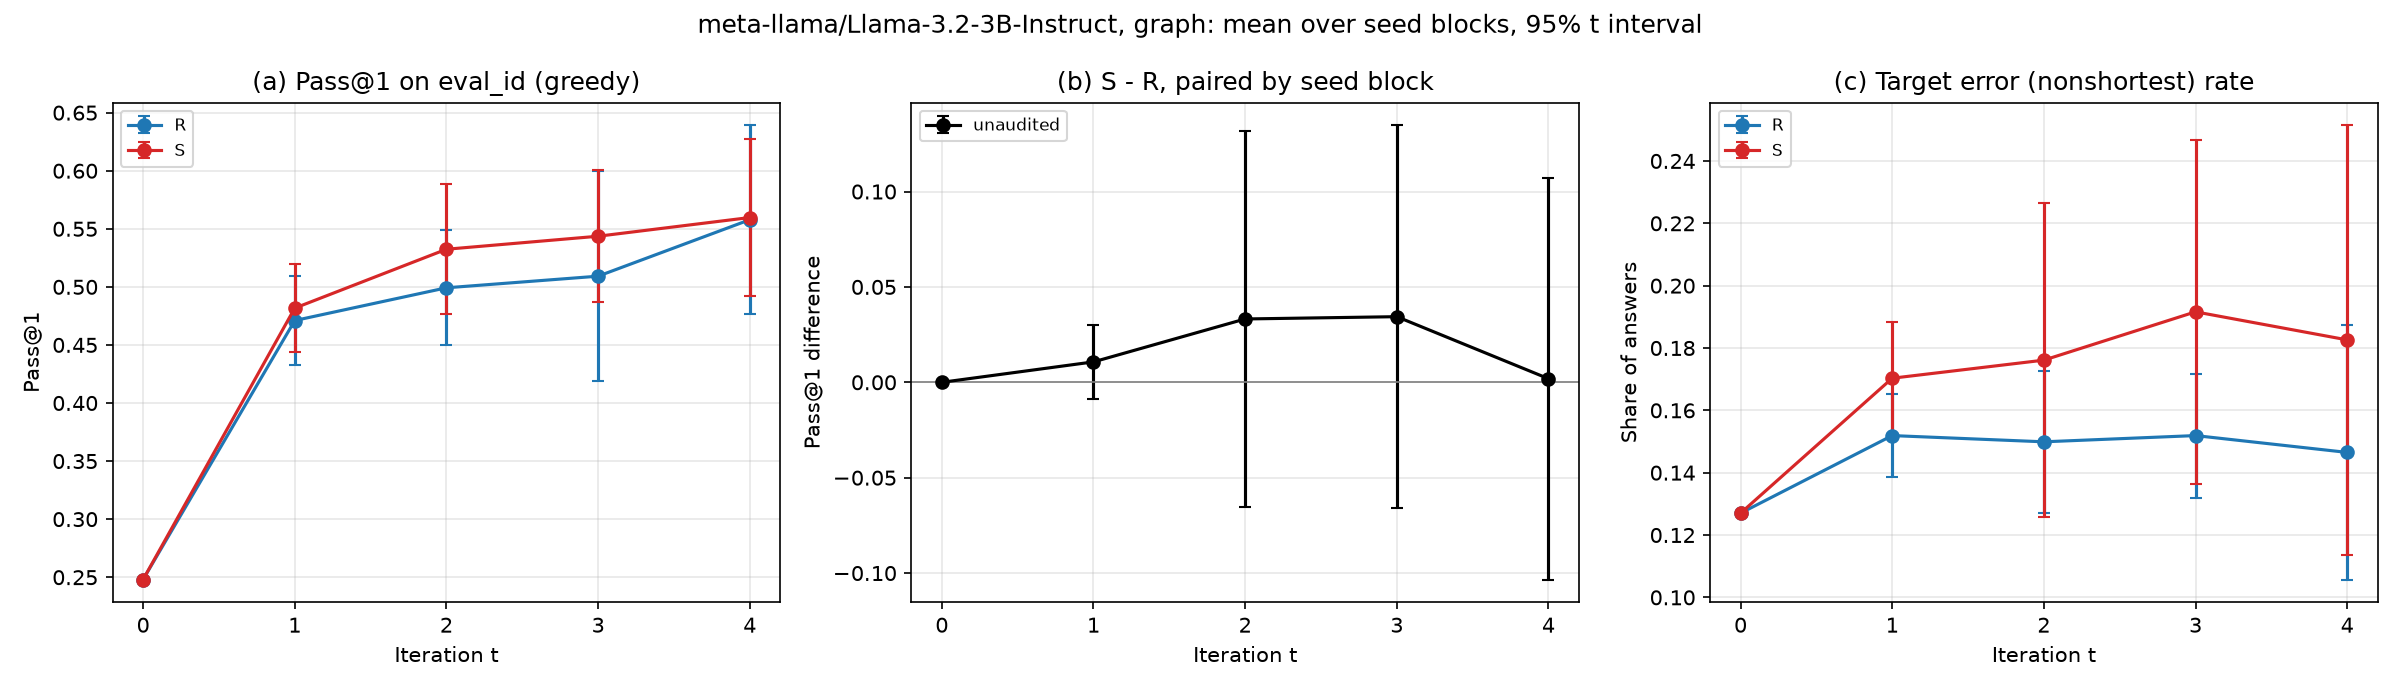
\includegraphics[width=0.90\linewidth]{figures/llama_four_round_raw/unaudited_eval_id_pass1.png}
\par\smallskip
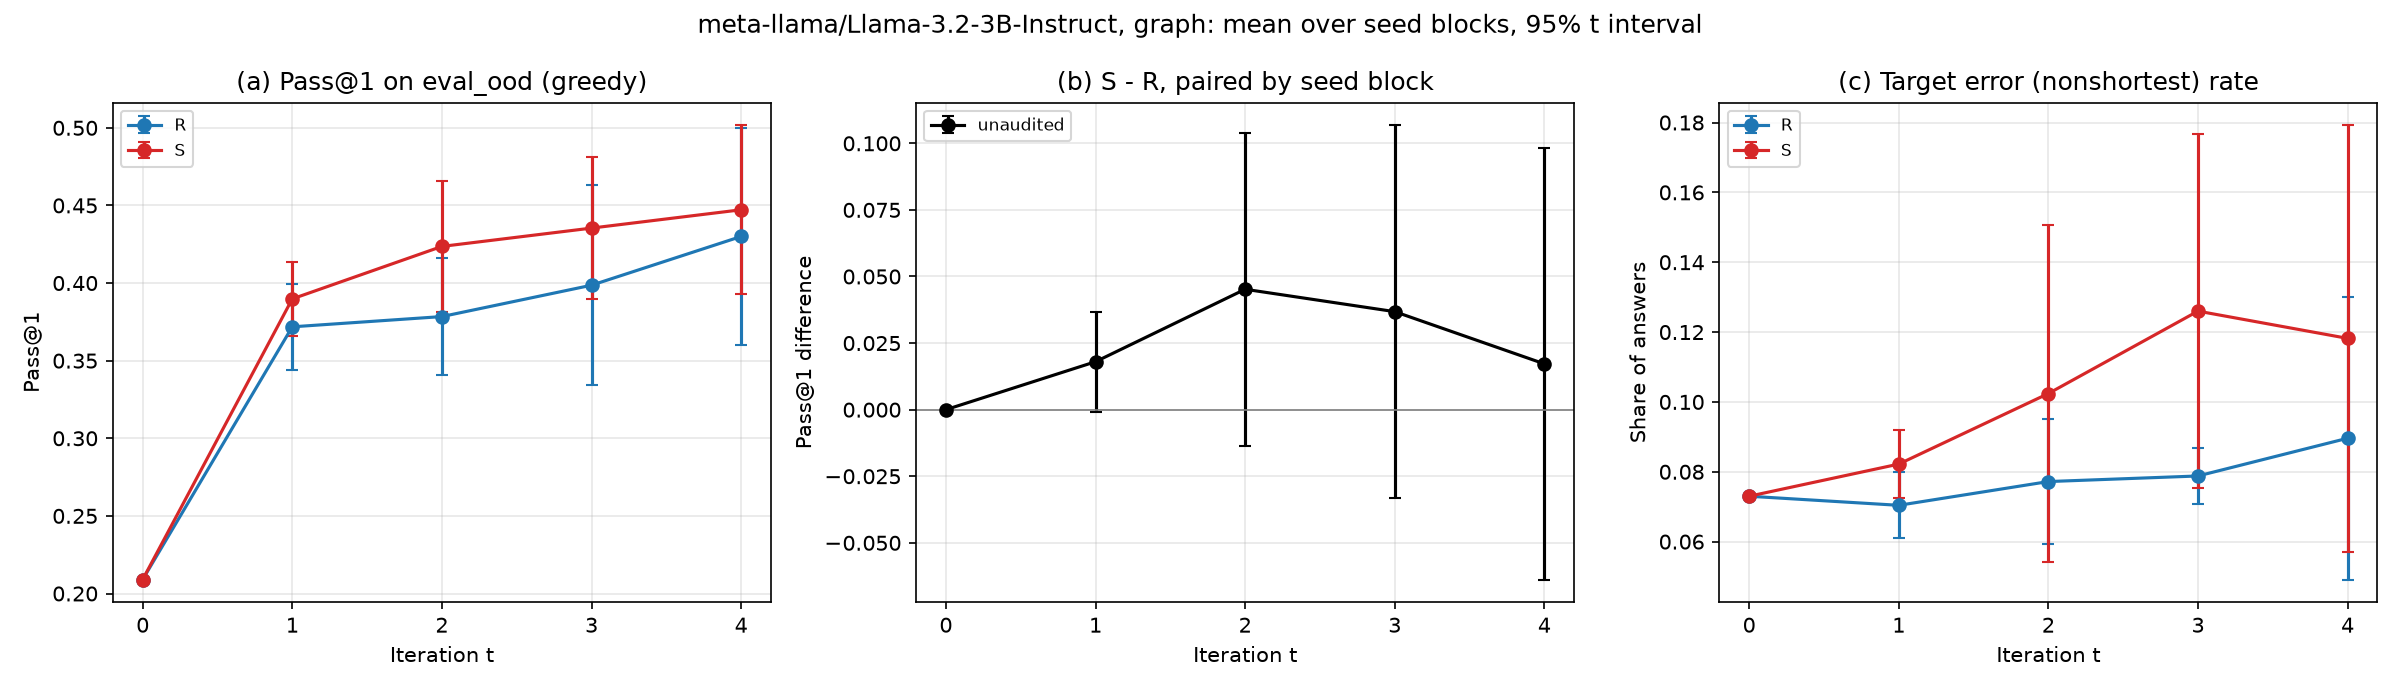
\includegraphics[width=0.90\linewidth]{figures/llama_four_round_raw/unaudited_eval_ood_pass1.png}
\caption{Original unaudited Llama-3.2-3B graph curves, ID (top) and OOD
(bottom), for rounds 0--4. The three panels show greedy Pass@1, paired
$S-R$ accuracy, and nonshortest-error incidence among all answers.}
\label{fig:llama-raw-unaudited}
\end{figure}

Both unaudited arms improve from the shared bases $0.248$ ID and
$0.209$ OOD. Round-four $R/S$ accuracy is $0.558/0.560$ ID and
$0.430/0.447$ OOD, with paired contrasts $0.002\pm0.105$ and
$0.017\pm0.081$.

\begin{figure}[H]
\centering
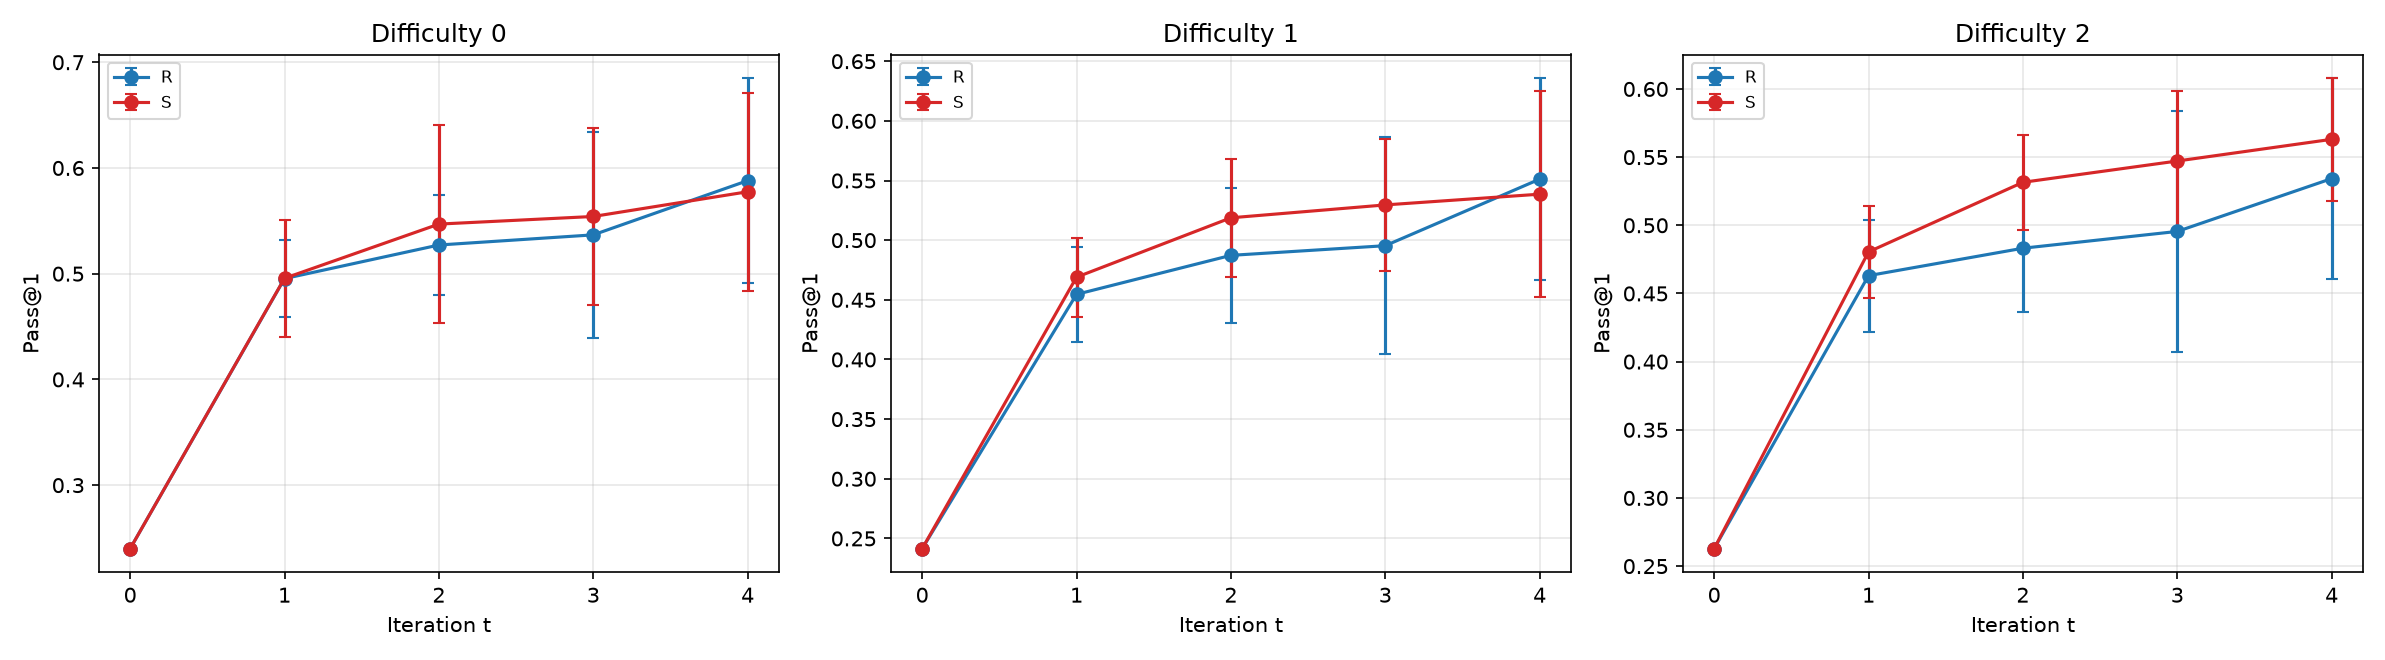
\includegraphics[width=0.90\linewidth]{figures/llama_four_round_raw/unaudited_eval_id_by_difficulty.png}
\par\smallskip
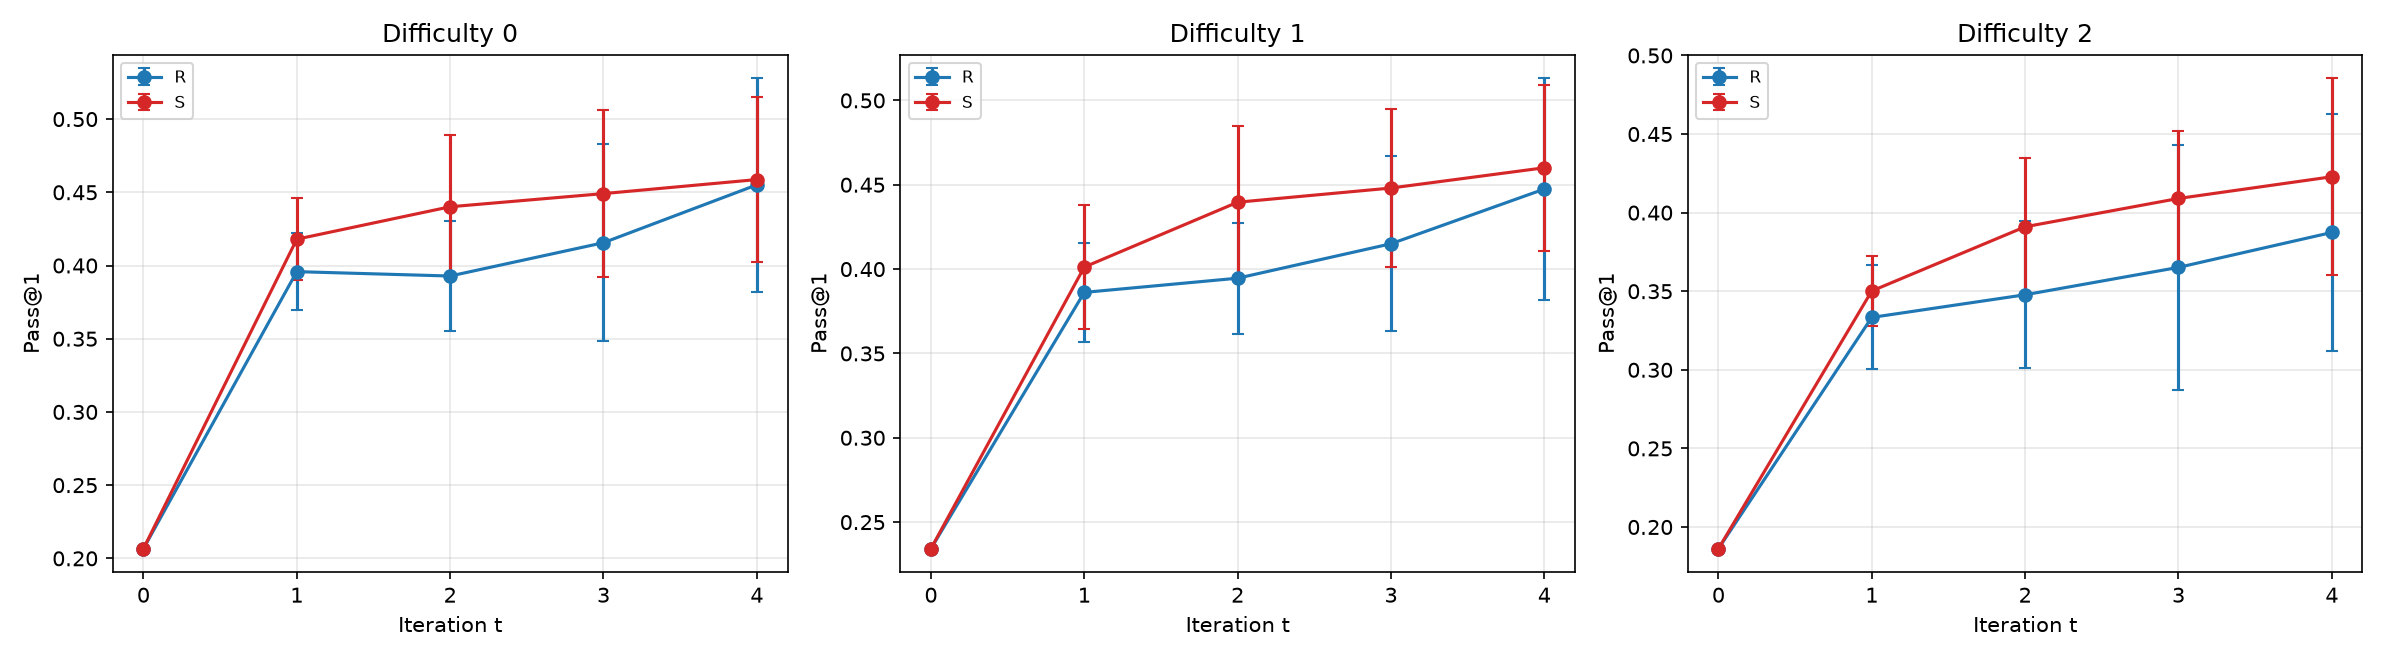
\includegraphics[width=0.90\linewidth]{figures/llama_four_round_raw/unaudited_eval_ood_by_difficulty.png}
\caption{Original unaudited Llama-3.2-3B graph accuracy by generator
difficulty stratum, ID (top) and OOD (bottom), for rounds 0--4.
Strata 0--2 run from left to right and contain $667/667/666$ ID
and $334/333/333$ OOD questions. Error bars use five paired blocks.}
\label{fig:llama-raw-unaudited-difficulty}
\end{figure}

These are fixed generator strata, not an established model-difficulty
ordering. The panel-specific vertical scales are retained, and differences
in the appearance of the curves do not constitute additional
difficulty-specific significance evidence.

\begin{figure}[H]
\centering
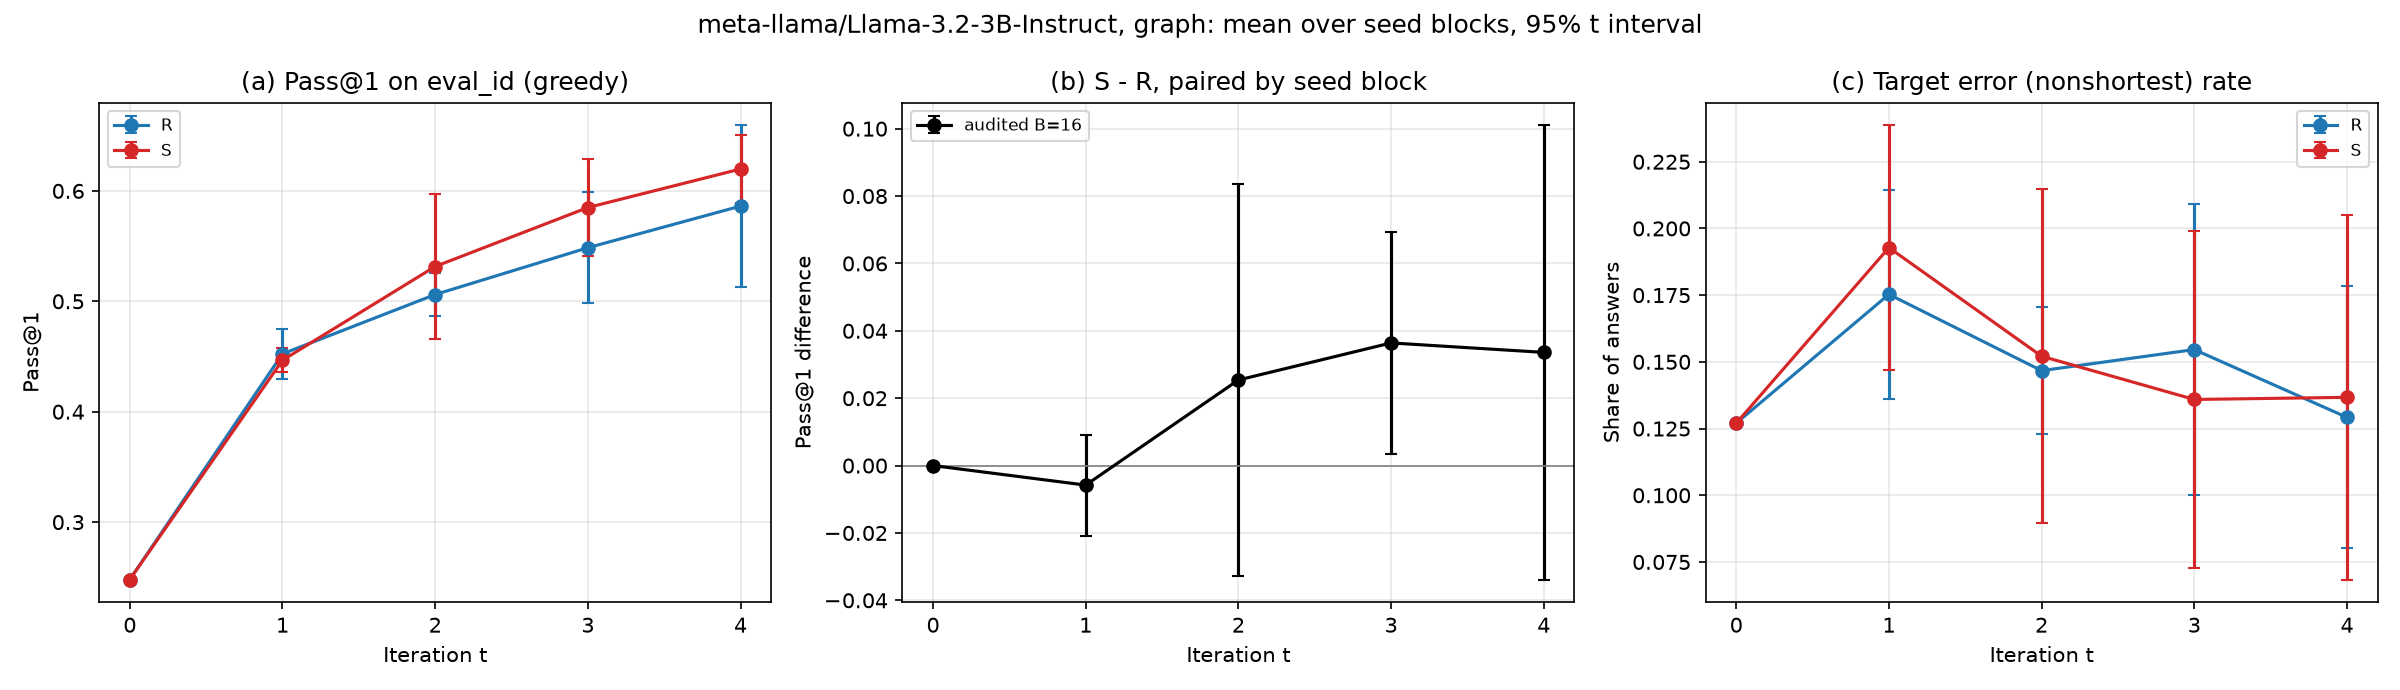
\includegraphics[width=0.90\linewidth]{figures/llama_four_round_raw/audited_eval_id_pass1.png}
\par\smallskip
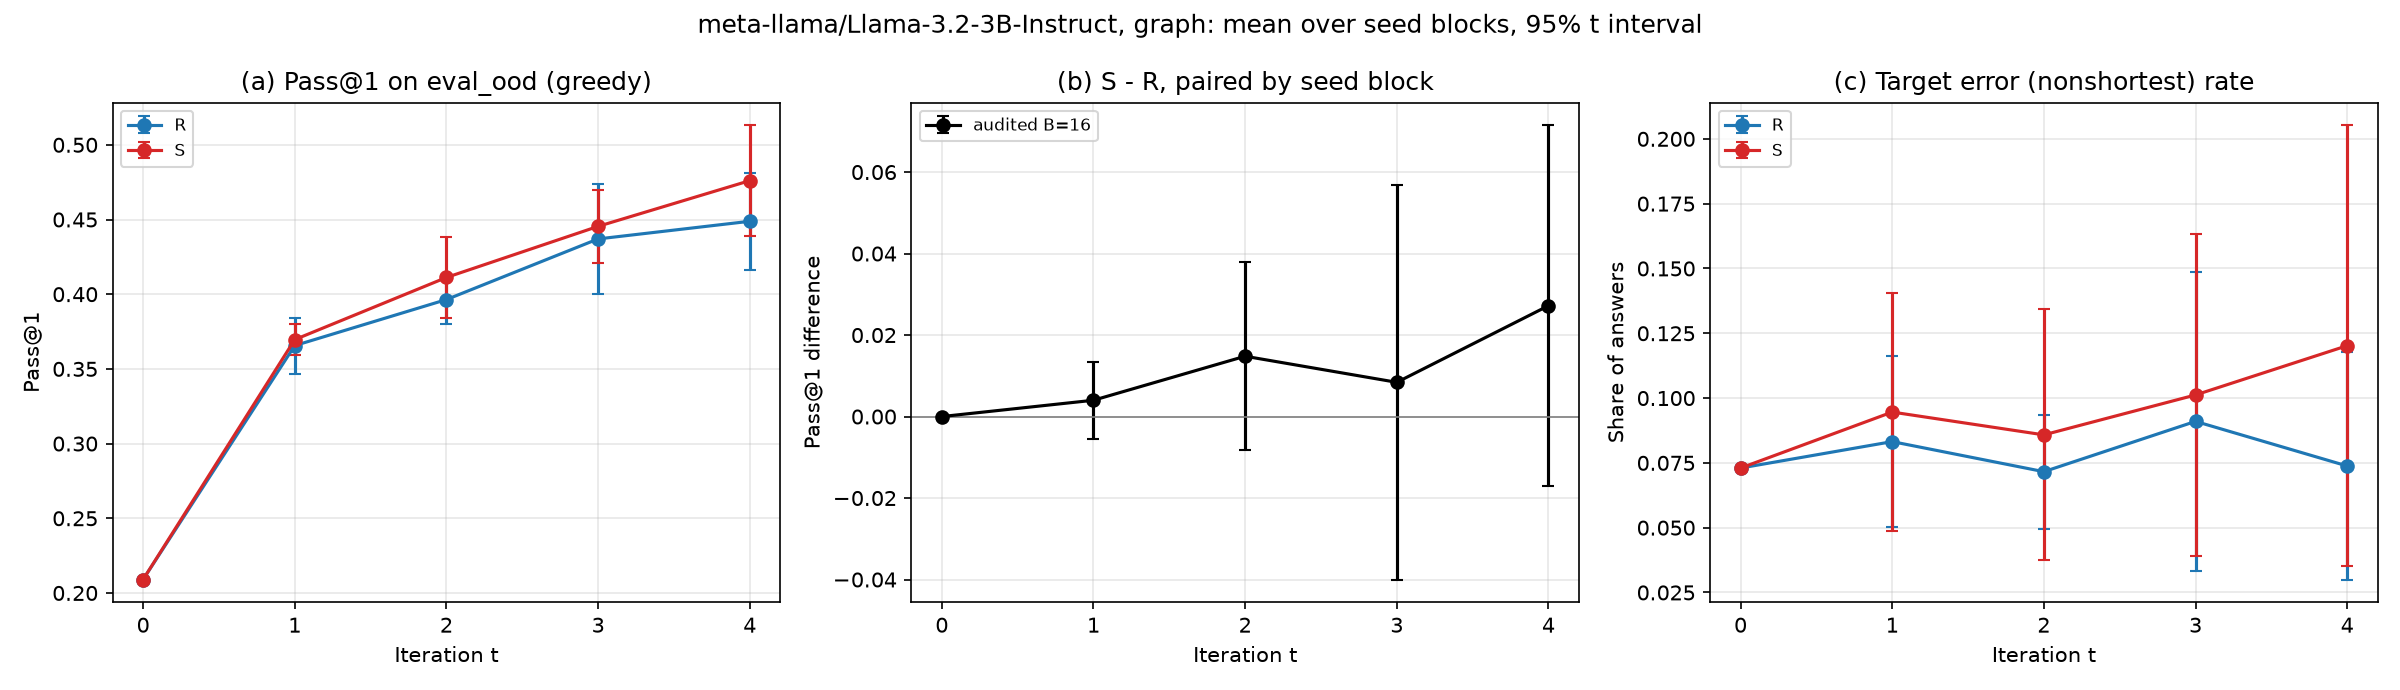
\includegraphics[width=0.90\linewidth]{figures/llama_four_round_raw/audited_eval_ood_pass1.png}
\caption{Original adaptive-audit Llama-3.2-3B graph curves, ID (top)
and OOD (bottom), with $B_{\rm qry}=16$ correctness queries per
arm-round. The panels show greedy Pass@1, paired $S-R$ accuracy,
and nonshortest-error incidence. Each audited arm spends 64 queries.}
\label{fig:llama-raw-audited}
\end{figure}

Audited round-four $R/S$ accuracy reaches $0.586/0.620$ ID and
$0.449/0.476$ OOD. The paired accuracy contrasts are
$0.034\pm0.067$ and $0.027\pm0.044$, respectively.
These are within-policy arm contrasts, not effects of auditing.

\begin{figure}[H]
\centering
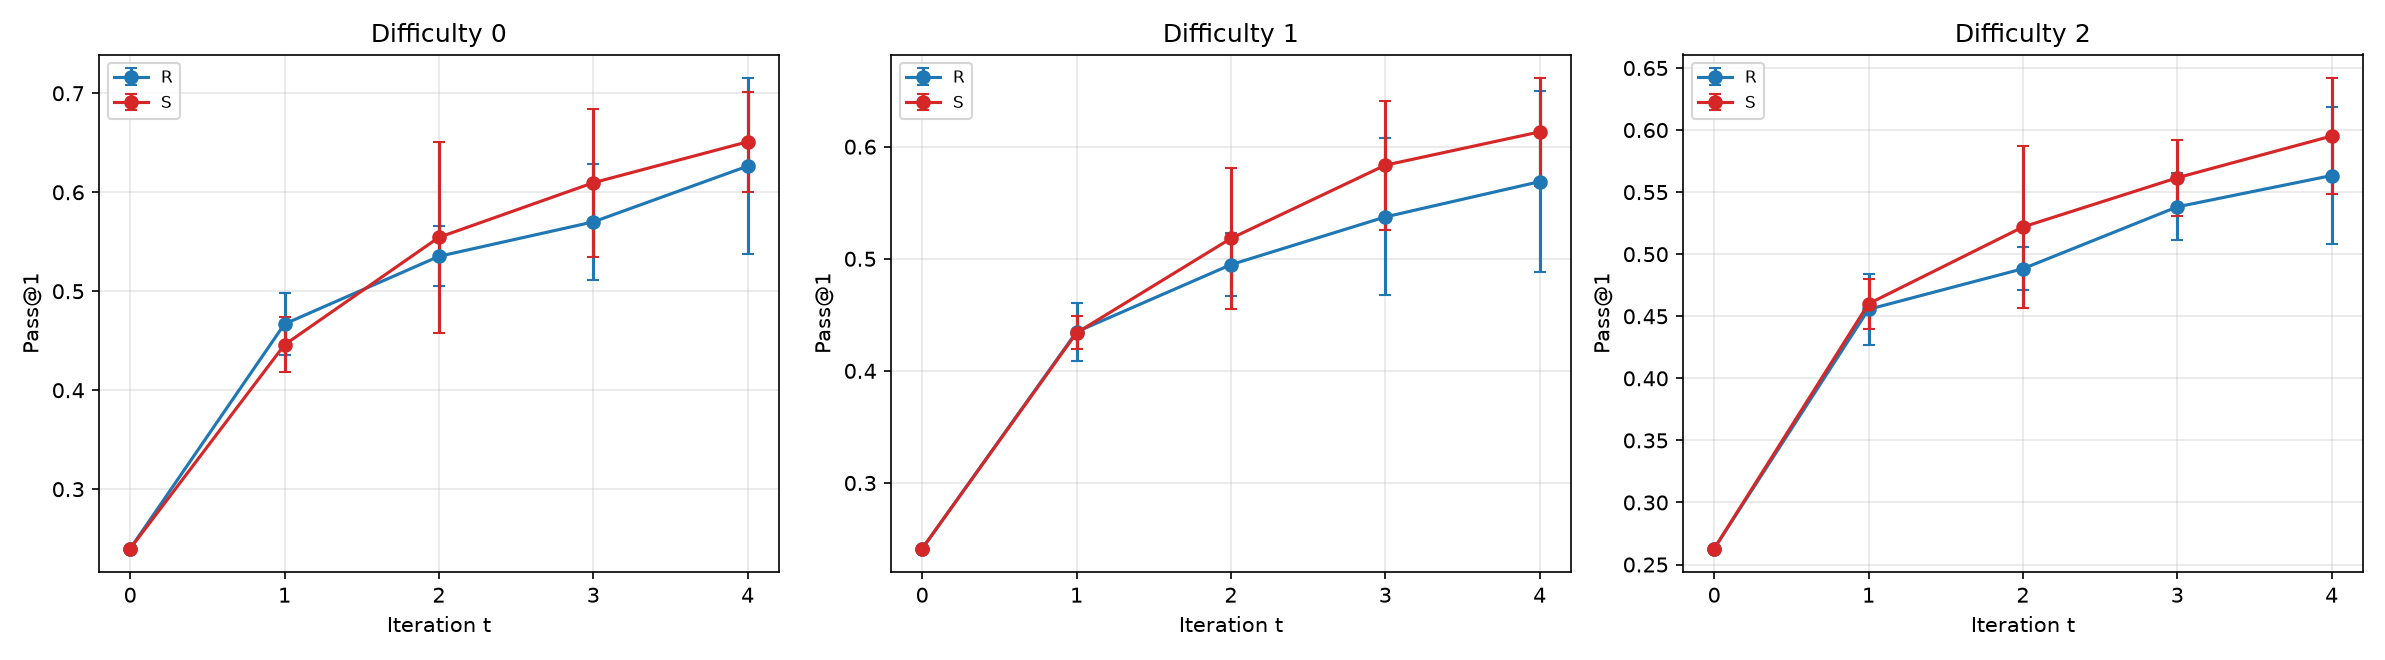
\includegraphics[width=0.90\linewidth]{figures/llama_four_round_raw/audited_eval_id_by_difficulty.png}
\par\smallskip
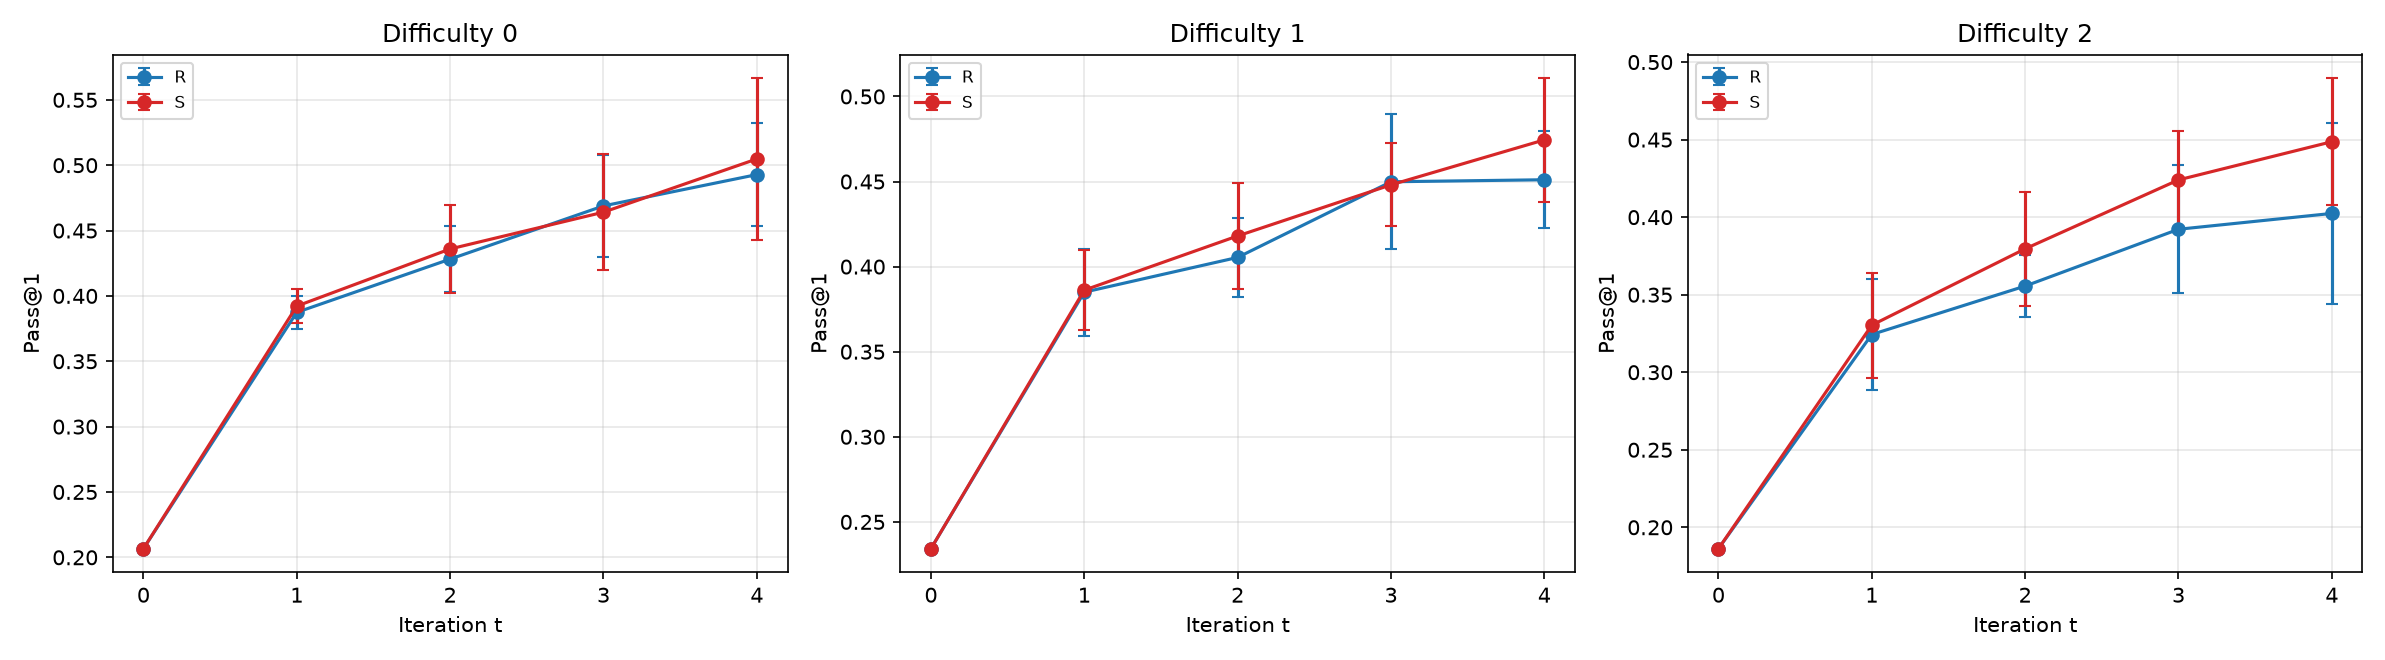
\includegraphics[width=0.90\linewidth]{figures/llama_four_round_raw/audited_eval_ood_by_difficulty.png}
\caption{Original adaptive-audit Llama-3.2-3B graph accuracy by
generator stratum, ID (top) and OOD (bottom), for rounds 0--4.
The fixed question strata and pointwise block-$t$ intervals follow
Figure~\ref{fig:llama-raw-unaudited-difficulty}.}
\label{fig:llama-raw-audited-difficulty}
\end{figure}

The audited curves show heterogeneous trajectories across the generator
strata. They retain separate vertical scales and use the same question
sets as the unaudited curves. This descriptive breakdown does not
establish stratum-specific audit benefits.

\begin{figure}[H]
\centering
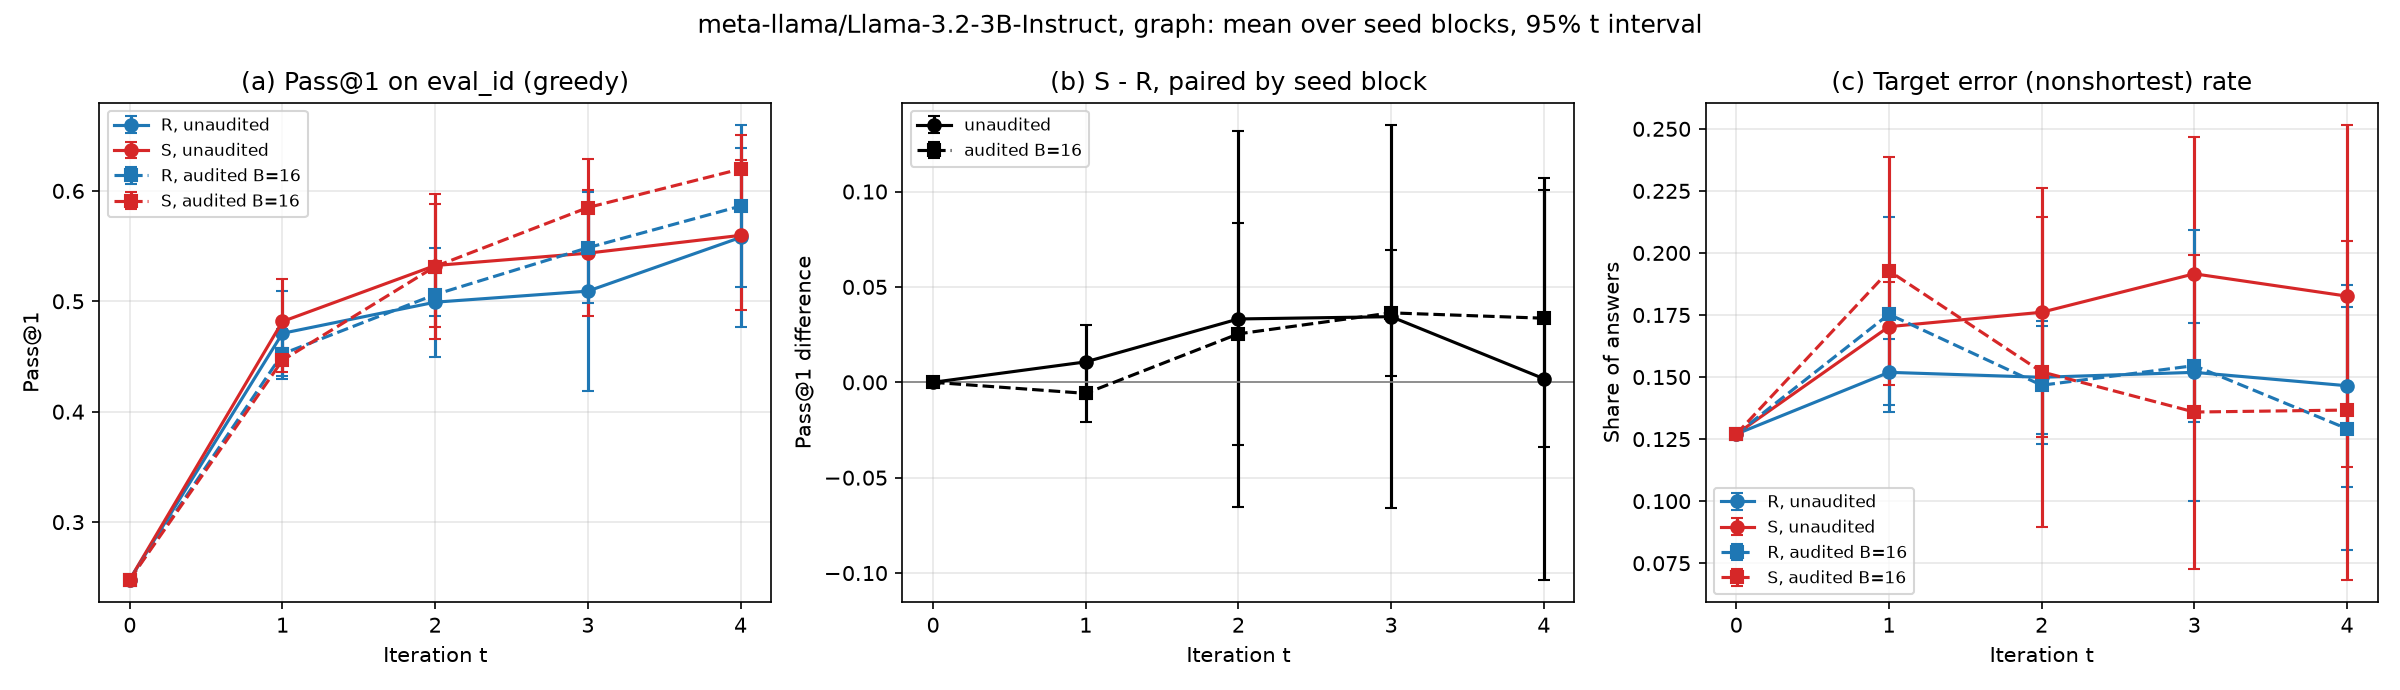
\includegraphics[width=0.90\linewidth]{figures/llama_four_round_raw/comparison_eval_id_pass1.png}
\par\smallskip
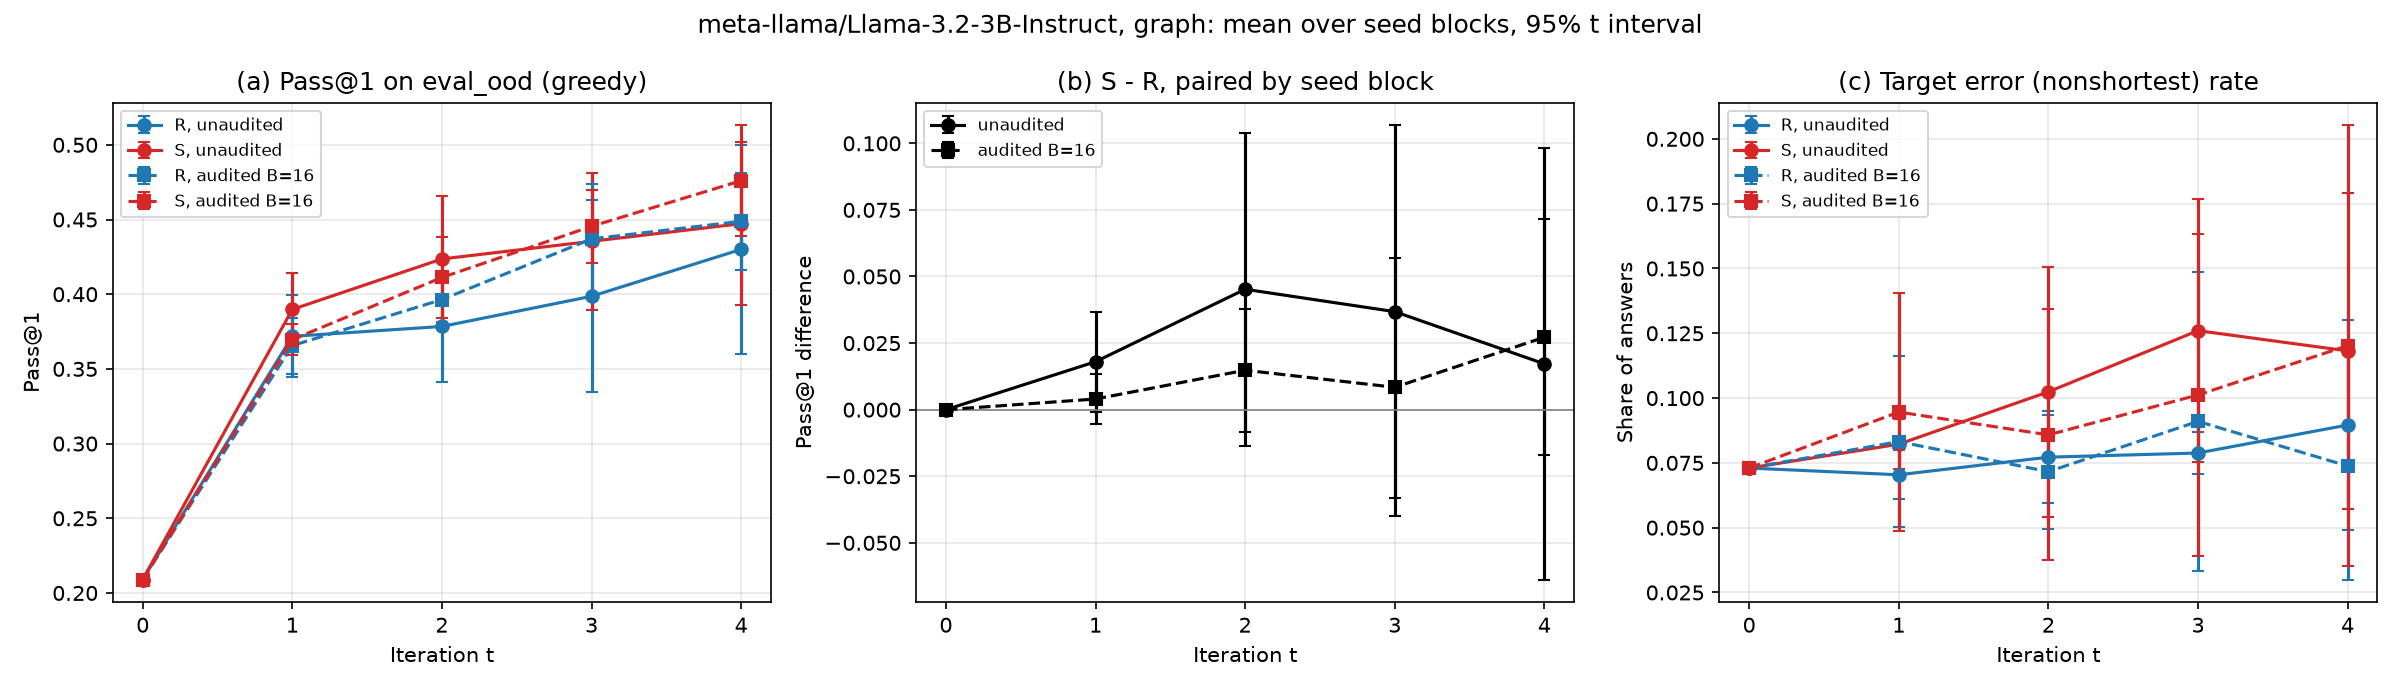
\includegraphics[width=0.90\linewidth]{figures/llama_four_round_raw/comparison_eval_ood_pass1.png}
\caption{Original joint comparison of unaudited and adaptive-audit
Llama-3.2-3B graph trajectories, ID (top) and OOD (bottom), for
rounds 0--4. Each middle panel reports paired $S-R$ accuracy
within each policy, not audited-minus-unaudited effects.}
\label{fig:llama-raw-comparison}
\label{fig:h100-id}
\label{fig:h100-ood}
\end{figure}

Auditing improves same-arm endpoint accuracy in mean
(Table~\ref{tab:audit-results}). Audited
OOD $S$ nonshortest incidence is $0.120$, versus $0.118$ without
auditing, so target-error suppression is not uniform.

\begin{figure}[H]
\centering
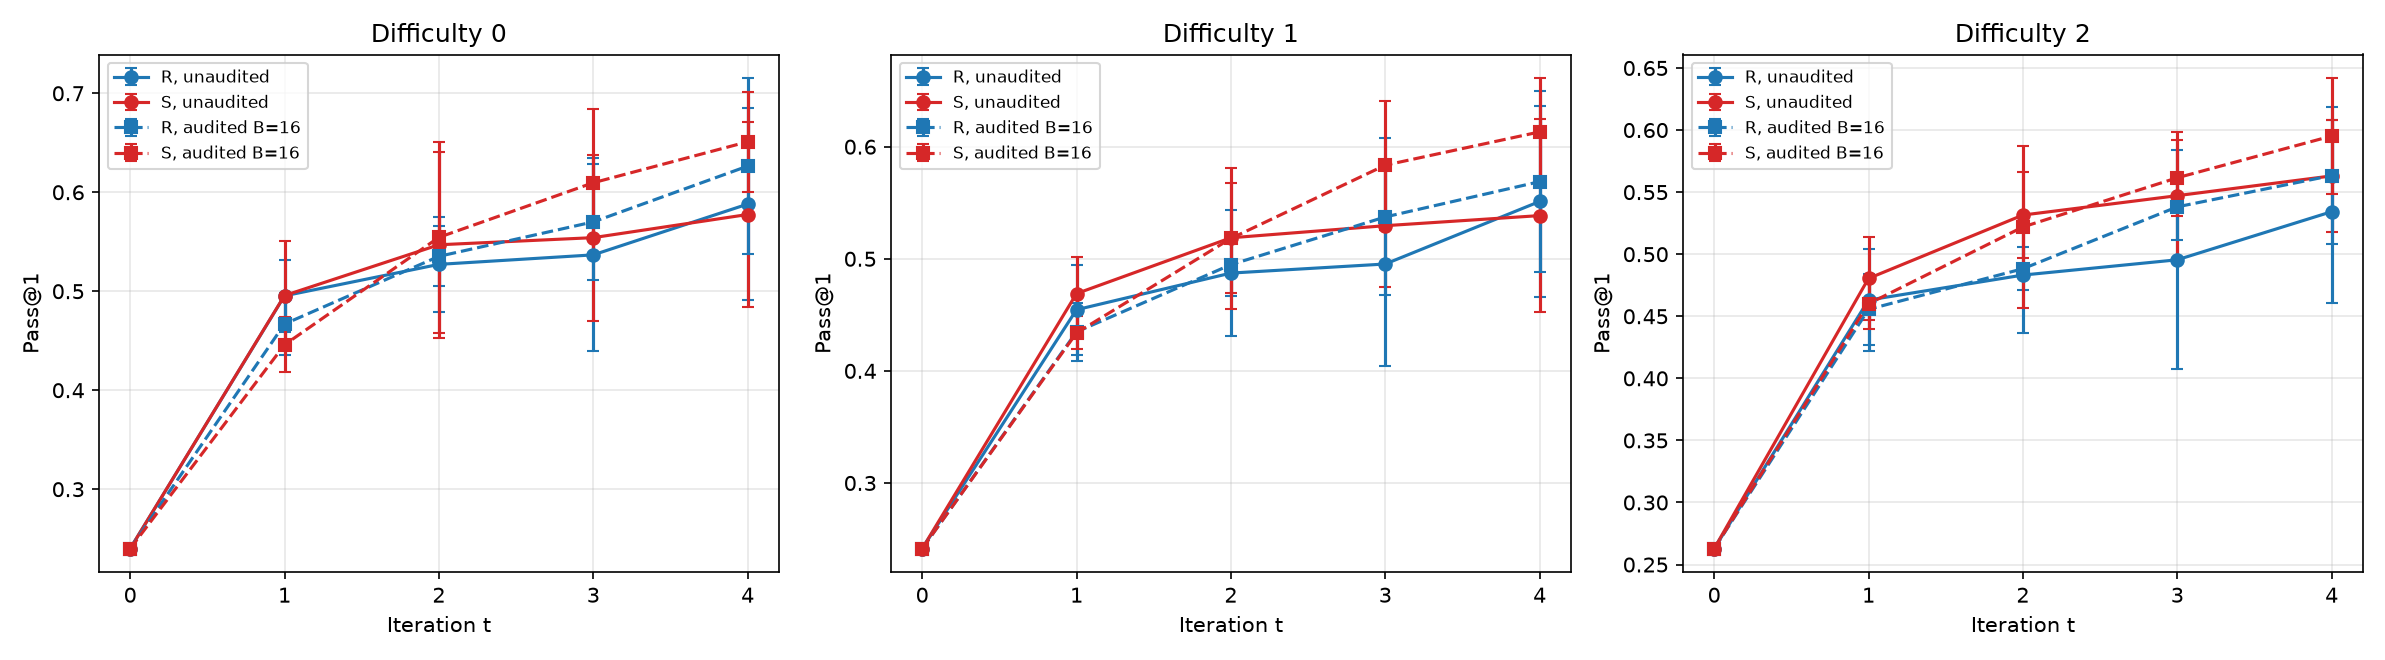
\includegraphics[width=0.90\linewidth]{figures/llama_four_round_raw/comparison_eval_id_by_difficulty.png}
\par\smallskip
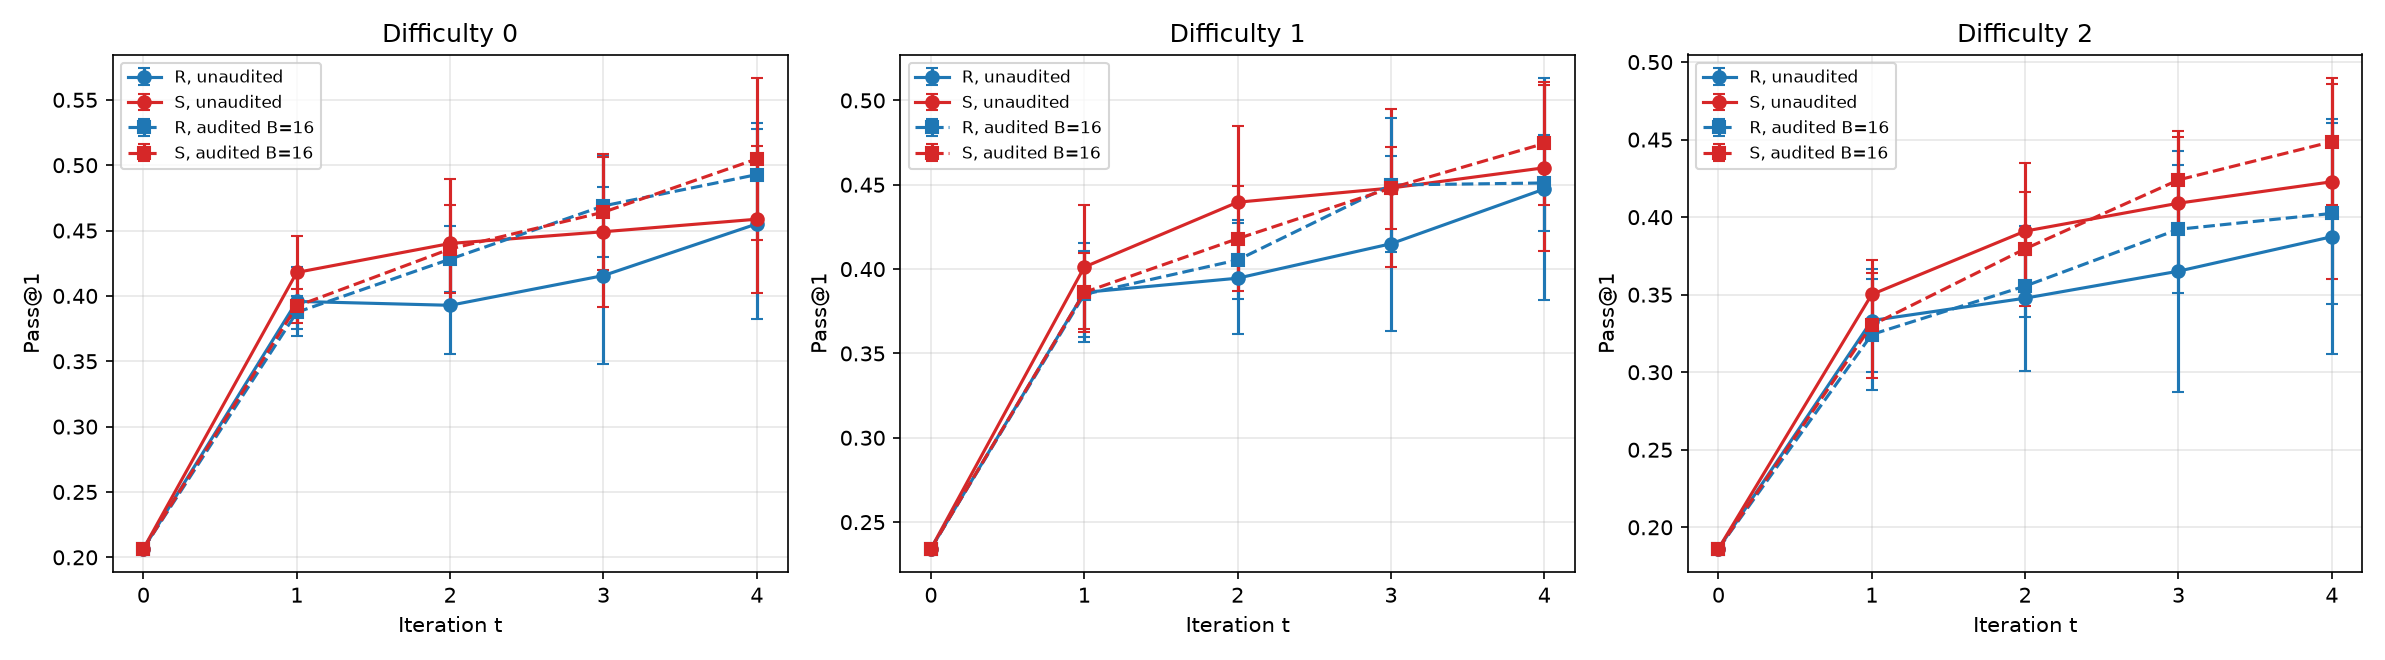
\includegraphics[width=0.90\linewidth]{figures/llama_four_round_raw/comparison_eval_ood_by_difficulty.png}
\caption{Original joint Llama-3.2-3B graph accuracy curves by
generator stratum, ID (top) and OOD (bottom), for rounds 0--4.
Both policies and both arms use the same question stratum at
each checkpoint. Counts and interval conventions follow
Figure~\ref{fig:llama-raw-unaudited-difficulty}.}
\label{fig:llama-raw-comparison-difficulty}
\label{fig:h100-difficulty}
\end{figure}

Both policies and both arms share the same question stratum at each
checkpoint. Separate vertical scales are retained, and the intervals
are not adjusted for comparisons across strata, rounds, or policies.
The joint curves complement the aggregate audit comparison without
providing an additional multiplicity-adjusted test.
\endgroup


\subsection{Shared audit and diagnostic conventions}
The finite-budget comparisons report correctness queries separately from
matching and evaluation labels. Retained rows, positive-weight rows, and
ESS measure different aspects of the training distribution; none alone
fixes optimizer effort. Within-policy $S-R$ contrasts and same-arm
audited-minus-unaudited changes answer different questions and are reported
separately for each model. All projections use a fixed initial reference
gradient and are surrogate diagnostics, not certificates of held-out
improvement. The population theorem analyzes a different auditing policy
and provides no direct guarantee for these adaptive finite-budget runs.

\subsection{Cross-task feasibility}
Table~\ref{tab:h100-feasibility} reports every block's round-one
pool statistics and eligible error-role prompts. Graph has exact-length
feasibility at $K=64$. The two arithmetic configurations deliberately
disable response-length matching; their counterfactual checks
fail exact-length matching at every $K$ in the ladder. This is a reported
protocol difference, not a post-hoc claim of exact-length arithmetic matching.
Raw-pool correctness/target counts in this table are distinct from
Table~\ref{tab:matching}'s eligible-pool rate denominators.
The added Qwen3-4B rows use independently rejudged original pools, with
exact-length error-role eligibility taken from matching certificates.
The arithmetic reference responses are bare canonical
integers (2--4 supervised tokens), whereas prompts request worked solutions
ending in \texttt{Answer: N}; projections can therefore reflect format changes.
The completed one-step graph outcomes and diagnostics are reported in
Tables~\ref{tab:one-step-heldout} and~\ref{tab:one-step-diagnostics}.

\begin{table}[H]
\caption{Round-one feasibility across five model/task pairs; audited siblings reuse the same pools. Each block has 16,384 sampled answers. Correctness and target counts use the full raw pool; matching excludes cut responses. $J_E$ counts prompts eligible for error-role matching at error fraction $0.25$, with exact length ($J_E^{\rm exact}$) or configured tolerance ($J_E^{\rm cfg}$). Qwen3-4B pool labels are independently rejudged; its $J_E$ values come from matching certificates. Graph permits $K=64$ with exact lengths. Arithmetic disables length matching; its exact-length ladder fails at $K=64,32,16$. These are feasibility checks, not held-out learning results.}
\label{tab:h100-feasibility}
\centering\small\setlength{\tabcolsep}{4pt}
\begin{tabular}{@{}llccccccc@{}}
\toprule
Task/model & Block & Correct (\%) & Cut & Target & $J_E^{\rm exact}$ & $J_E^{\rm cfg}$ & Length & $K$\\
\midrule
Graph / Qwen3-1.7B & b00 & 50.31 & 27 & 2357 & 27 & 27 & exact & 64\\
Graph / Qwen3-1.7B & b01 & 50.60 & 29 & 2351 & 38 & 38 & exact & 64\\
Graph / Qwen3-1.7B & b02 & 50.43 & 33 & 2322 & 32 & 32 & exact & 64\\
Graph / Qwen3-1.7B & b03 & 50.83 & 30 & 2354 & 31 & 31 & exact & 64\\
Graph / Qwen3-1.7B & b04 & 50.50 & 29 & 2346 & 28 & 28 & exact & 64\\
Graph / Llama-3B & b00 & 23.49 & 147 & 2095 & 184 & 184 & exact & 64\\
Graph / Llama-3B & b01 & 23.66 & 138 & 2112 & 180 & 180 & exact & 64\\
Graph / Llama-3B & b02 & 23.22 & 121 & 2095 & 178 & 178 & exact & 64\\
Graph / Llama-3B & b03 & 23.25 & 153 & 2140 & 188 & 188 & exact & 64\\
Graph / Llama-3B & b04 & 23.43 & 132 & 2124 & 192 & 192 & exact & 64\\
Arithmetic / Llama-3B & b00 & 74.48 & 0 & 74 & 2 & 30 & off & 64\\
Arithmetic / Llama-3B & b01 & 74.78 & 0 & 81 & 2 & 32 & off & 64\\
Arithmetic / Llama-3B & b02 & 74.71 & 2 & 71 & 1 & 17 & off & 64\\
Arithmetic / Llama-3B & b03 & 74.66 & 0 & 74 & 0 & 28 & off & 64\\
Arithmetic / Llama-3B & b04 & 74.83 & 2 & 87 & 1 & 33 & off & 64\\
Arithmetic / Llama-1B & b00 & 42.35 & 100 & 69 & 1 & 54 & off & 64\\
Arithmetic / Llama-1B & b01 & 42.03 & 111 & 69 & 2 & 45 & off & 64\\
Arithmetic / Llama-1B & b02 & 42.13 & 84 & 63 & 2 & 43 & off & 64\\
Arithmetic / Llama-1B & b03 & 42.30 & 90 & 75 & 2 & 55 & off & 64\\
Arithmetic / Llama-1B & b04 & 41.75 & 87 & 70 & 0 & 48 & off & 64\\
\addlinespace
Graph / Qwen3-4B & b00 & 63.02 & 9 & 3545 & 16 & 16 & exact & 64\\
Graph / Qwen3-4B & b01 & 63.01 & 7 & 3561 & 25 & 25 & exact & 64\\
Graph / Qwen3-4B & b02 & 63.23 & 10 & 3530 & 21 & 21 & exact & 64\\
Graph / Qwen3-4B & b03 & 63.29 & 5 & 3523 & 30 & 30 & exact & 64\\
Graph / Qwen3-4B & b04 & 63.02 & 9 & 3531 & 30 & 30 & exact & 64\\
\bottomrule
\end{tabular}
\end{table}


\subsection{Validation scope}
We independently reconstruct numerical summaries and figures from the
saved count and scalar records. The checks cover experiment completion,
shared initial pools and adapters, round-one matching constraints and
acceptance rates, checkpoint error counts and difficulty aggregation,
evaluation-protocol consistency, query and optimizer-step accounting,
and agreement with the plotting summaries. Overlapping Llama held-out
records agree across the initial and extended graph studies.
For the initial series, these checks do not independently rejudge responses,
reload checkpoints, or reconstruct unavailable gradient tensors and weights.
Qwen3-4B validation additionally rejudges original pools and audited held-out
answers, as detailed in Section~\ref{app:qwen4b-four-round}.

\subsection{Roundwise pre- and post-audit true-positive rates}
\label{app:roundwise-tpr}
Table~\ref{tab:h100-tpr} reports all four rounds of the completed graph
comparison. For each block, condition, arm, and round, $N^+$ counts correct
responses in that round's original pool after excluding truncated responses.
The pre-audit, retained, and positive-weight rates are
\[
 \mathrm{TPR}_{\rm pre}=\frac{48}{N^+},\qquad
 \mathrm{TPR}_{\rm ret}=\frac{C'}{N^+},\qquad
 \mathrm{TPR}_{w>0}=\frac{C'_{w>0}}{N^+},
\]
where $C'$ counts retained correct responses and $C'_{w>0}$ counts those
with positive training weight, irrespective of its magnitude. Auditing
keeps the same denominator.
All 40 audited arm-rounds retain the 48 selected correct responses, so
$\mathrm{TPR}_{\rm ret}=\mathrm{TPR}_{\rm pre}$; reliability weighting can
nevertheless reduce $\mathrm{TPR}_{w>0}$. In unaudited runs, unit weights
make selection TPR equal to positive-weight TPR.

Later pools come from each arm's preceding checkpoint, so their $N^+$
and TPRs need not agree across arms or conditions. With the correct quota
fixed at 48, a larger correct pool lowers selection TPR without implying
lower model accuracy. These rates are distinct from subset precision and
held-out Pass@1. We check block-level numerators and denominators for
80 completed arm-rounds and 40 audit reports. This establishes consistency
of the saved counts, not independent rejudging of unavailable raw responses.

The Llama rates are collected with its other four-round results in
Table~\ref{tab:h100-tpr}; Qwen rates appear in
Tables~\ref{tab:qwen-audit} and~\ref{tab:qwen4b-audit}.
\subsection{Qwen3-1.7B: four-round graph replication}
\label{app:qwen-four-round}

The Qwen3-1.7B unaudited and adaptive-audit graph comparisons each have
five complete paired blocks and both held-out splits. The primary analysis
uses the fixed rounds 0--4 horizon; round-eight contrasts are reported at
the end of this subsection, without selecting a best checkpoint.

Qwen3-1.7B response generation uses temperature $1.3$ and
top-$p=1$. LoRA, matching quotas, optimizer settings, prompt/sample counts,
and audit budget follow the four-round protocol in Section~\ref{sec:experiments}.
There are 40 trained checkpoints per policy in the selected horizon,
plus one shared base, each evaluated greedily on 2,000 ID and 1,000 OOD
questions. Policies bind the same initial adapter, dataset, and round-one
pools. Table~\ref{tab:qwen-matching} reports the nontruncated-pool
TPR/FPR and exact initial matching controls; $R$ already contains 6--12
nonshortest errors among its 16 accepted errors.

\begin{table}[H]
\caption{Qwen3-1.7B graph round-one matching certificate, common to the audited and unaudited runs and their one-step reuse. $N^+/N^-$ exclude truncated answers; $R/S$ share correct IDs, task IDs, 48/16 correct/error quotas and exact supervised response lengths. Later checkpoint-dependent pools are not jointly matched.}
\label{tab:qwen-matching}
\centering\small\setlength{\tabcolsep}{3pt}
\begin{tabular}{@{}lllllll@{}}
\toprule
Block & $N^+/N^-$ & Cut & TPR/FPR & Yield & Target hits $R/S$ & Controls\\
\midrule
b00 & 8243/8114 & 27 & 0.005823/0.001972 & 0.003913 & 12/16 & pass\\
b01 & 8290/8065 & 29 & 0.005790/0.001984 & 0.003913 & 6/16 & pass\\
b02 & 8262/8089 & 33 & 0.005810/0.001978 & 0.003914 & 12/16 & pass\\
b03 & 8328/8026 & 30 & 0.005764/0.001994 & 0.003913 & 9/16 & pass\\
b04 & 8274/8081 & 29 & 0.005801/0.001980 & 0.003913 & 6/16 & pass\\
\bottomrule
\end{tabular}
\end{table}

\begin{table}[H]
\caption{Qwen3-1.7B graph endpoints after four rounds. Target rates count nonshortest answers among all evaluated questions. Paired differences use five blocks, with descriptive 95\% block-$t$ half-widths; no multiplicity adjustment is applied.}
\label{tab:qwen-endpoints}
\centering\small\setlength{\tabcolsep}{3pt}
\begin{tabular}{@{}lllllll@{}}
\toprule
Split & Policy & Base & Pass@1 $R/S$ & $S-R$ Pass@1 & Target $R/S$ & $S-R$ target\\
\midrule
ID & None & 0.4995 & 0.556/0.553 & $-0.003\pm0.044$ & 0.103/0.171 & $0.068\pm0.039$\\
ID & B=16 & 0.4995 & 0.533/0.551 & $0.017\pm0.093$ & 0.129/0.158 & $0.029\pm0.074$\\
OOD & None & 0.3470 & 0.363/0.389 & $0.026\pm0.038$ & 0.057/0.124 & $0.066\pm0.038$\\
OOD & B=16 & 0.3470 & 0.362/0.386 & $0.024\pm0.038$ & 0.073/0.102 & $0.029\pm0.043$\\
\bottomrule
\end{tabular}
\end{table}

\begin{table}[H]
\caption{Qwen3-1.7B four-round graph policy endpoints, with five paired blocks. Errors are mean fractions. $Q$ counts correctness-audit queries per arm/block, excluding matching and evaluation labels; steps are cumulative updates (mean and range). $\Delta$ is audited-minus-unaudited error with a descriptive paired 95\% block-$t$ interval on fixed questions (negative favors auditing). Models are not pooled. One-step outcomes are separate (Table~\ref{tab:one-step-heldout}).}
\label{tab:qwen17-policy-endpoints}
\centering\small\setlength{\tabcolsep}{3pt}
\begin{tabular}{@{}llcccccc@{}}
\toprule
Policy & Arm & $Q$ & Steps & ID error & OOD error & \shortstack{$\Delta$ID\\(95\% CI)} & \shortstack{$\Delta$OOD\\(95\% CI)}\\
\midrule
\multicolumn{8}{@{}l}{\textbf{Qwen3-1.7B}}\\
Base & --- & 0 & 0 & 0.5005 & 0.6530 & --- & ---\\
Unaudited & R & 0 & 64 & 0.444 & 0.637 & --- & ---\\
Unaudited & S & 0 & 64 & 0.447 & 0.611 & --- & ---\\
Adaptive, B=16 & R & 64 & 48.0 (37--56) & 0.467 & 0.638 & $0.022\;[-0.026,0.071]$ & $0.001\;[-0.037,0.039]$\\
Adaptive, B=16 & S & 64 & 53.2 (46--57) & 0.449 & 0.614 & $0.002\;[-0.082,0.086]$ & $0.003\;[-0.054,0.060]$\\
\bottomrule
\end{tabular}
\end{table}

\begin{figure}[H]
\centering
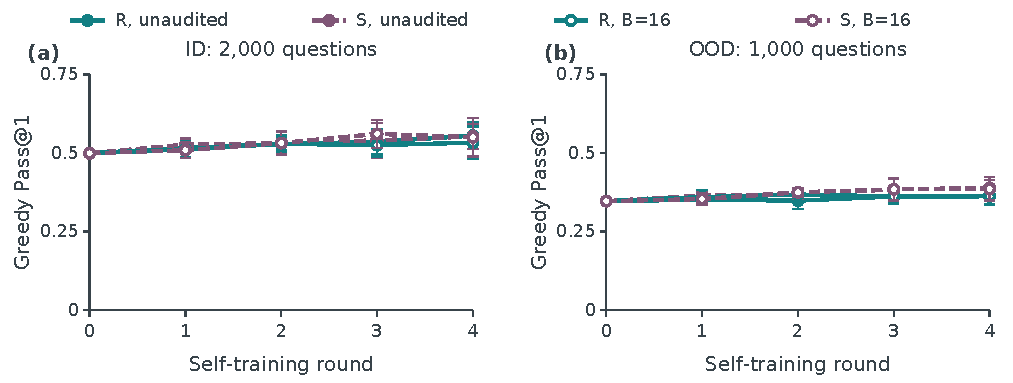
\includegraphics[width=0.8\linewidth]{figures/graph_extensions/qwen_accuracy.pdf}
\caption{Four-round Qwen3-1.7B graph self-training improves mean accuracy in both arms
from shared base accuracy $0.4995$ ID/$0.347$ OOD. Unaudited $R/S$ reach
$0.556/0.553$ ID and $0.363/0.389$ OOD; with 16 correctness queries per
arm-round, they reach $0.533/0.551$ and $0.362/0.386$, respectively.
Bars are pointwise 95\% block-$t$ intervals over five blocks on fixed
questions. Round zero has one shared checkpoint; only rounds 0--4 are shown.
Nonshortest-error incidence is reported in Figure~\ref{fig:qwen-target-errors}.}
\label{fig:qwen-four-round}
\end{figure}


\begin{figure}[H]
\centering
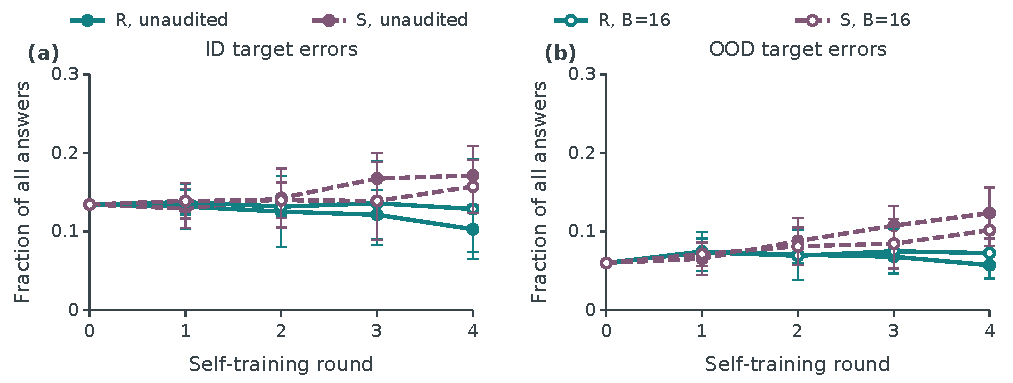
\includegraphics[width=0.8\linewidth]{figures/graph_extensions/qwen_target_errors.pdf}
\caption{Qwen3-1.7B four-round nonshortest-error incidence among all answers.
Unaudited $R/S$ reach $0.103/0.171$ ID and $0.057/0.124$ OOD at round four;
unaudited target-incidence contrasts are $0.068\pm0.039$ ID and $0.066\pm0.038$ OOD.
Audited target-incidence contrasts are $0.029\pm0.074$ ID and
$0.029\pm0.043$ OOD. Bars are
pointwise 95\% block-$t$ intervals over five blocks; the common base has
no independent block replication. Only rounds 0--4 are shown.}
\label{fig:qwen-target-errors}
\end{figure}

Accuracy and error composition need not tell the same story. In the
unaudited Qwen comparison, the round-four nonshortest fractions are
$0.103/0.171$ ID and $0.057/0.124$ OOD for $R/S$. Both paired target
contrasts have descriptive intervals above zero, despite accuracy
contrasts $-0.003\pm0.044$ ID and $0.026\pm0.038$ OOD. This is a
task-signature finding, not a measurement of high-influence errors or
the opposite-direction construction. The audited target contrasts are
$0.029\pm0.074$ ID and $0.029\pm0.043$ OOD.
All rounds and endpoint blocks appear in Tables~\ref{tab:qwen-rounds}
and~\ref{tab:qwen-blocks}. These multiple descriptive comparisons are
not multiplicity-adjusted confirmatory tests.

\begin{table}[H]
\caption{Qwen3-1.7B graph trajectories restricted to the original four-round protocol. Entries are means $\pm$ pointwise 95\% block-$t$ half-widths. The base is one common checkpoint, not five independent fits.}
\label{tab:qwen-rounds}
\centering\small\setlength{\tabcolsep}{3pt}
\begin{tabular}{@{}lllllllll@{}}
\toprule
Split & Policy & Round & Pass@1 $R$ & Pass@1 $S$ & Pass@1 $S-R$ & Target $R$ & Target $S$ & Target $S-R$\\
\midrule
ID & Base & 0 & 0.4995 & 0.4995 & --- & 0.135 & 0.135 & ---\\
ID & None & 1 & $0.517\pm0.017$ & $0.527\pm0.019$ & $0.010\pm0.012$ & $0.132\pm0.029$ & $0.129\pm0.024$ & $-0.003\pm0.012$\\
ID & None & 2 & $0.529\pm0.029$ & $0.532\pm0.037$ & $0.003\pm0.035$ & $0.126\pm0.045$ & $0.143\pm0.038$ & $0.017\pm0.043$\\
ID & None & 3 & $0.536\pm0.040$ & $0.541\pm0.055$ & $0.005\pm0.039$ & $0.121\pm0.031$ & $0.168\pm0.032$ & $0.046\pm0.022$\\
ID & None & 4 & $0.556\pm0.043$ & $0.553\pm0.040$ & $-0.003\pm0.044$ & $0.103\pm0.029$ & $0.171\pm0.037$ & $0.068\pm0.039$\\
ID & B=16 & 1 & $0.513\pm0.027$ & $0.509\pm0.024$ & $-0.003\pm0.017$ & $0.138\pm0.016$ & $0.139\pm0.022$ & $0.002\pm0.009$\\
ID & B=16 & 2 & $0.529\pm0.021$ & $0.532\pm0.012$ & $0.003\pm0.015$ & $0.132\pm0.014$ & $0.140\pm0.022$ & $0.008\pm0.020$\\
ID & B=16 & 3 & $0.526\pm0.039$ & $0.561\pm0.045$ & $0.036\pm0.056$ & $0.136\pm0.053$ & $0.139\pm0.049$ & $0.003\pm0.073$\\
ID & B=16 & 4 & $0.533\pm0.051$ & $0.551\pm0.062$ & $0.017\pm0.093$ & $0.129\pm0.064$ & $0.158\pm0.034$ & $0.029\pm0.074$\\
OOD & Base & 0 & 0.3470 & 0.3470 & --- & 0.060 & 0.060 & ---\\
OOD & None & 1 & $0.352\pm0.011$ & $0.366\pm0.015$ & $0.014\pm0.021$ & $0.075\pm0.025$ & $0.065\pm0.021$ & $-0.009\pm0.007$\\
OOD & None & 2 & $0.349\pm0.026$ & $0.369\pm0.016$ & $0.020\pm0.020$ & $0.071\pm0.032$ & $0.088\pm0.029$ & $0.017\pm0.026$\\
OOD & None & 3 & $0.362\pm0.022$ & $0.385\pm0.034$ & $0.023\pm0.022$ & $0.068\pm0.016$ & $0.108\pm0.025$ & $0.040\pm0.015$\\
OOD & None & 4 & $0.363\pm0.026$ & $0.389\pm0.025$ & $0.026\pm0.038$ & $0.057\pm0.017$ & $0.124\pm0.032$ & $0.066\pm0.038$\\
OOD & B=16 & 1 & $0.360\pm0.023$ & $0.354\pm0.017$ & $-0.006\pm0.016$ & $0.074\pm0.017$ & $0.071\pm0.015$ & $-0.002\pm0.010$\\
OOD & B=16 & 2 & $0.368\pm0.011$ & $0.375\pm0.013$ & $0.007\pm0.015$ & $0.069\pm0.009$ & $0.081\pm0.024$ & $0.012\pm0.026$\\
OOD & B=16 & 3 & $0.362\pm0.016$ & $0.385\pm0.035$ & $0.023\pm0.031$ & $0.075\pm0.028$ & $0.085\pm0.032$ & $0.010\pm0.044$\\
OOD & B=16 & 4 & $0.362\pm0.028$ & $0.386\pm0.037$ & $0.024\pm0.038$ & $0.073\pm0.032$ & $0.102\pm0.020$ & $0.029\pm0.043$\\
\bottomrule
\end{tabular}
\end{table}

\begin{table}[H]
\caption{Qwen3-1.7B four-round graph endpoint blocks. Each paired cell reports $R/S$; models and splits are not pooled as replicate blocks.}
\label{tab:qwen-blocks}
\centering\small\setlength{\tabcolsep}{3pt}
\begin{tabular}{@{}llllll@{}}
\toprule
Policy & Block & ID Pass@1 & OOD Pass@1 & ID target & OOD target\\
\midrule
None & b00 & 0.558/0.571 & 0.358/0.401 & 0.098/0.153 & 0.055/0.108\\
None & b01 & 0.534/0.585 & 0.340/0.409 & 0.106/0.144 & 0.064/0.111\\
None & b02 & 0.561/0.543 & 0.369/0.391 & 0.100/0.153 & 0.056/0.096\\
None & b03 & 0.517/0.502 & 0.353/0.356 & 0.138/0.214 & 0.074/0.150\\
None & b04 & 0.609/0.565 & 0.396/0.389 & 0.073/0.192 & 0.037/0.153\\
B=16 & b00 & 0.482/0.531 & 0.348/0.366 & 0.189/0.142 & 0.098/0.088\\
B=16 & b01 & 0.535/0.525 & 0.352/0.367 & 0.118/0.171 & 0.067/0.091\\
B=16 & b02 & 0.515/0.637 & 0.345/0.420 & 0.128/0.120 & 0.071/0.091\\
B=16 & b03 & 0.540/0.545 & 0.399/0.417 & 0.158/0.192 & 0.093/0.120\\
B=16 & b04 & 0.595/0.514 & 0.368/0.361 & 0.051/0.163 & 0.034/0.119\\
\bottomrule
\end{tabular}
\end{table}


The same-arm audit changes in Table~\ref{tab:qwen-audit-change} are
negative in mean but imprecise. Audited arms spend 64 correctness queries
each and take mean cumulative steps $48.0$ for $R$ and $53.2$ for $S$,
versus 64 without auditing. This differs from Llama's positive mean
accuracy changes and does not support a uniform audit benefit.
Table~\ref{tab:qwen-audit} gives each round's retained volume,
positive-weight coverage, ESS, projection, and TPRs. Querying removes
errors, so all 48 correct rows survive deletion in every audited
arm-round; reliability weighting can still assign zero weight to correct
rows. Retained-row TPR equals pre-audit TPR, whereas positive-weight TPR
can be smaller. Each uses its own original nontruncated pool denominator,
as in Section~\ref{app:roundwise-tpr}. ESS is checked against saved
audit summaries, not independently reconstructed from omitted weights.

\begin{table}[H]
\caption{Qwen3-1.7B same-arm audited-minus-unaudited accuracy changes at round four (positive favors auditing), with paired 95\% block-$t$ half-widths. Each unaudited arm takes 64 steps. Auditing spends 16 correctness queries per arm-round but changes weights, positive-weight training volume, and actual optimizer effort.}
\label{tab:qwen-audit-change}
\centering\small\setlength{\tabcolsep}{3pt}
\begin{tabular}{@{}lllll@{}}
\toprule
Arm & Queries & Audited steps: mean [range] & ID accuracy change & OOD accuracy change\\
\midrule
R & 64 & 48.0 [37,56] & $-0.022\pm0.049$ & $-0.001\pm0.038$\\
S & 64 & 53.2 [46,57] & $-0.002\pm0.084$ & $-0.003\pm0.057$\\
\bottomrule
\end{tabular}
\end{table}

\begin{table}[H]
\caption{Qwen3-1.7B graph update and audit readouts, means over five blocks. $K\prime$ counts retained rows, $n^+$ positive-weight rows, and ESS uses saved weights. TPR columns are percentages on each original nontruncated pool: pre-audit $48/N^+$ and positive-weight correct count divided by $N^+$. All 48 correct rows survive deletion, so retained-row post-audit TPR equals pre-audit TPR. Unaudited rows have unit weights. The projection uses the fixed initial reference gradient and is not measured task risk.}
\label{tab:qwen-audit}
\centering\small\setlength{\tabcolsep}{3pt}
\begin{tabular}{@{}llllllllll@{}}
\toprule
Round & Policy & Arm & $h^T\Delta\theta_t$ & Steps & $K\prime$ & $n^+$ & ESS & Pre TPR (\%) & Positive TPR (\%)\\
\midrule
1 & None & R & $-0.0668$ & 16.0 & 64.0 & 64.0 & 64.00 & 0.5798 & 0.5798\\
1 & None & S & $-0.0654$ & 16.0 & 64.0 & 64.0 & 64.00 & 0.5798 & 0.5798\\
1 & B=16 & R & $-0.0625$ & 13.2 & 60.6 & 51.2 & 45.22 & 0.5798 & 0.5050\\
1 & B=16 & S & $-0.0535$ & 13.2 & 60.6 & 51.2 & 45.22 & 0.5798 & 0.5050\\
2 & None & R & $-0.0298$ & 16.0 & 64.0 & 64.0 & 64.00 & 0.5452 & 0.5452\\
2 & None & S & $-0.0286$ & 16.0 & 64.0 & 64.0 & 64.00 & 0.5301 & 0.5301\\
2 & B=16 & R & $-0.0179$ & 9.4 & 58.4 & 36.2 & 31.07 & 0.5468 & 0.3394\\
2 & B=16 & S & $-0.0024$ & 14.2 & 60.0 & 56.0 & 42.33 & 0.5503 & 0.5119\\
3 & None & R & $-0.0428$ & 16.0 & 64.0 & 64.0 & 64.00 & 0.5492 & 0.5492\\
3 & None & S & $-0.0365$ & 16.0 & 64.0 & 64.0 & 64.00 & 0.5480 & 0.5480\\
3 & B=16 & R & $-0.0070$ & 13.2 & 60.2 & 51.0 & 42.93 & 0.5407 & 0.4599\\
3 & B=16 & S & $-0.0391$ & 13.0 & 60.6 & 50.4 & 43.38 & 0.5401 & 0.4513\\
4 & None & R & $-0.0309$ & 16.0 & 64.0 & 64.0 & 64.00 & 0.5220 & 0.5220\\
4 & None & S & $-0.0158$ & 16.0 & 64.0 & 64.0 & 64.00 & 0.5193 & 0.5193\\
4 & B=16 & R & $-0.0108$ & 12.2 & 59.6 & 47.2 & 39.57 & 0.5276 & 0.4322\\
4 & B=16 & S & $-0.0115$ & 12.8 & 59.8 & 49.8 & 40.04 & 0.5049 & 0.4270\\
\bottomrule
\end{tabular}
\end{table}


\begingroup
\let\figure\RSIappendixfigure
\let\endfigure\RSIendappendixfigure
\subsubsection{Original four-round Qwen figures}
\label{app:qwen-raw-figures}

Figures~\ref{fig:qwen-raw-unaudited}--\ref{fig:qwen-raw-comparison-difficulty}
show the original Qwen3-1.7B plots for rounds 0--4.
The unaudited and audited runs are shown separately and together,
including their difficulty-stratified curves. The plotted observations
are the same as those summarized in Figure~\ref{fig:qwen-four-round}
and Tables~\ref{tab:qwen-endpoints} and~\ref{tab:qwen-rounds}; these
plots are not additional experiments. Each uses the same 2,000 ID
or 1,000 OOD questions across checkpoints and five paired blocks.
Error bars are pointwise, descriptive 95\% block-$t$ intervals;
round zero is one shared base checkpoint, not five independent fits.
The underlying observations and intervals are unchanged.

\begin{figure}[H]
\centering
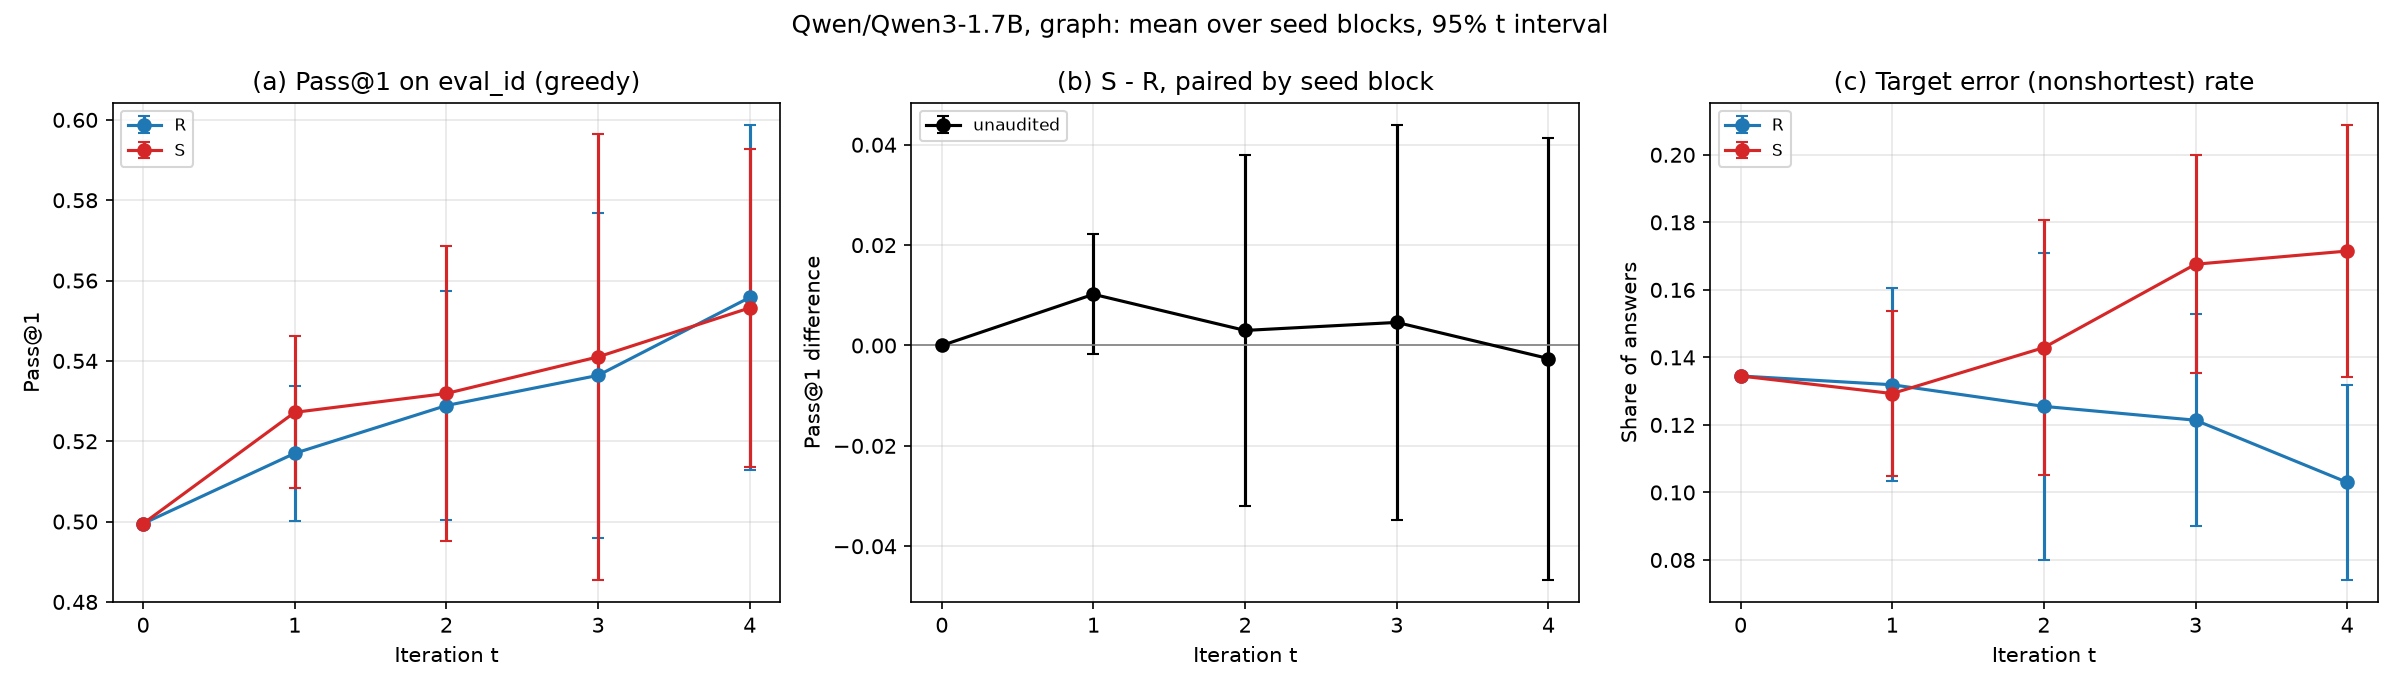
\includegraphics[width=0.90\linewidth]{figures/qwen_four_round_raw/unaudited_eval_id_pass1.png}
\par\smallskip
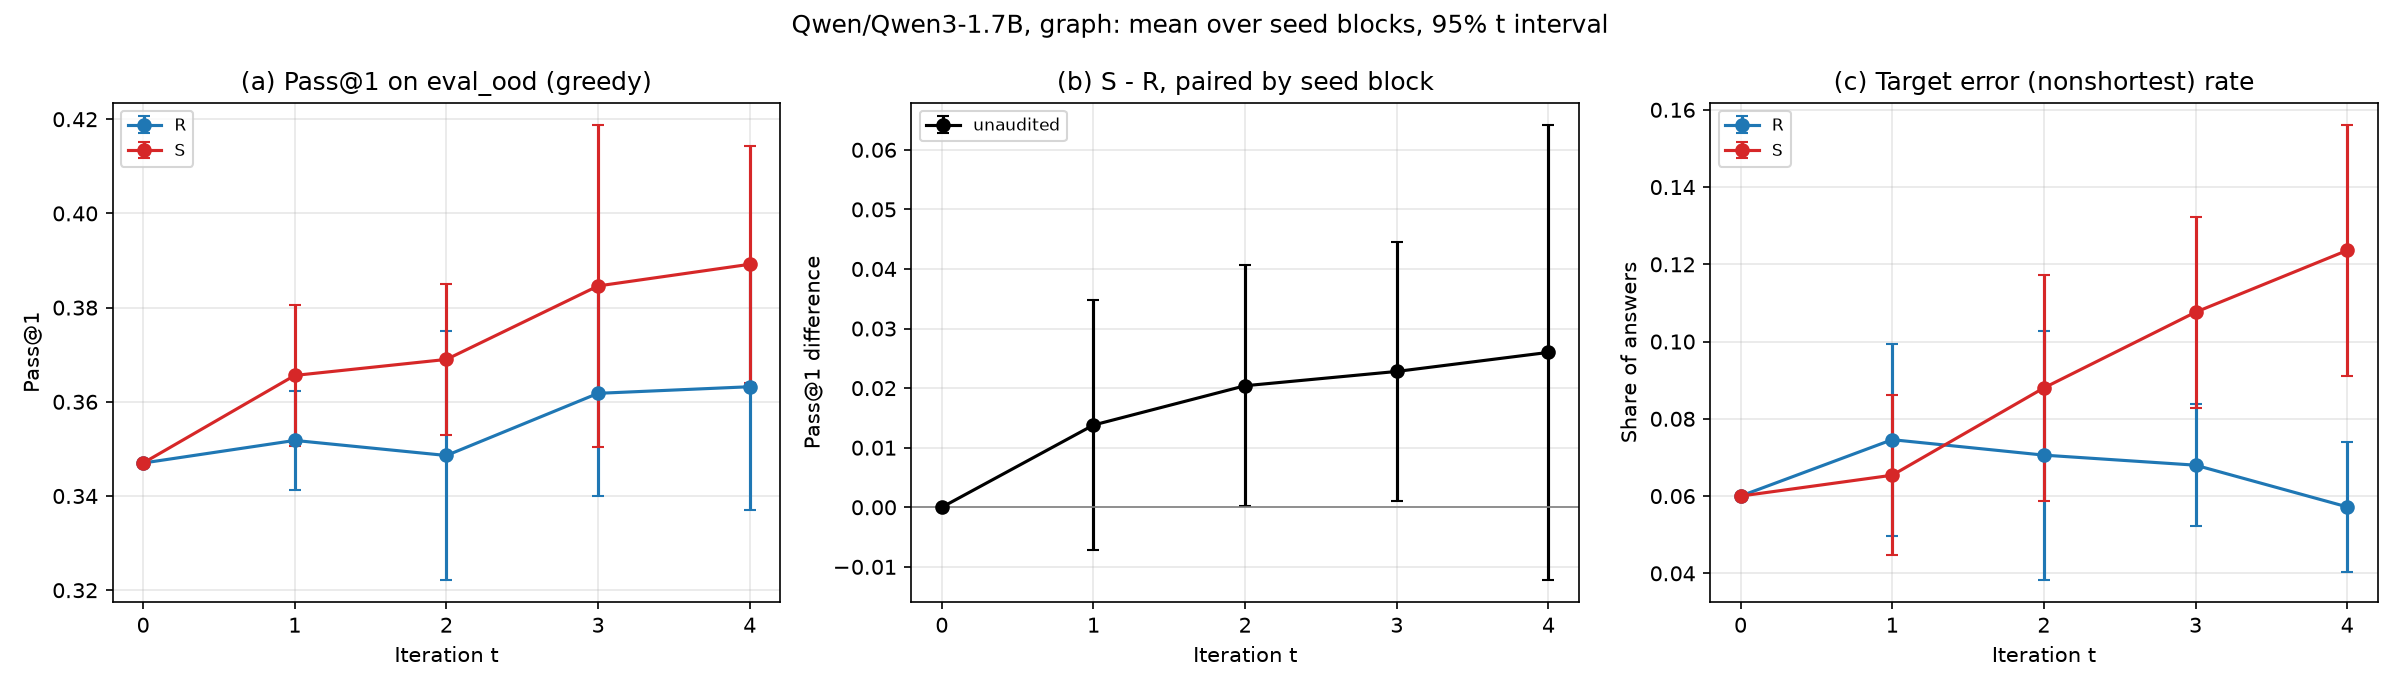
\includegraphics[width=0.90\linewidth]{figures/qwen_four_round_raw/unaudited_eval_ood_pass1.png}
\caption{Original unaudited Qwen3-1.7B graph curves, ID (top) and OOD
(bottom), for rounds 0--4. The three panels show greedy Pass@1, paired
$S-R$ accuracy, and nonshortest-error incidence among all answers.}
\label{fig:qwen-raw-unaudited}
\end{figure}

The unaudited arms reach round-four accuracy $0.556/0.553$ ID and
$0.363/0.389$ OOD, up from the common bases $0.4995$ and $0.3470$.
Nonshortest-error contrasts are $0.068\pm0.039$ ID and
$0.066\pm0.038$ OOD. Thus similar aggregate accuracy can coexist
with a difference in the composition of incorrect answers.

\begin{figure}[H]
\centering
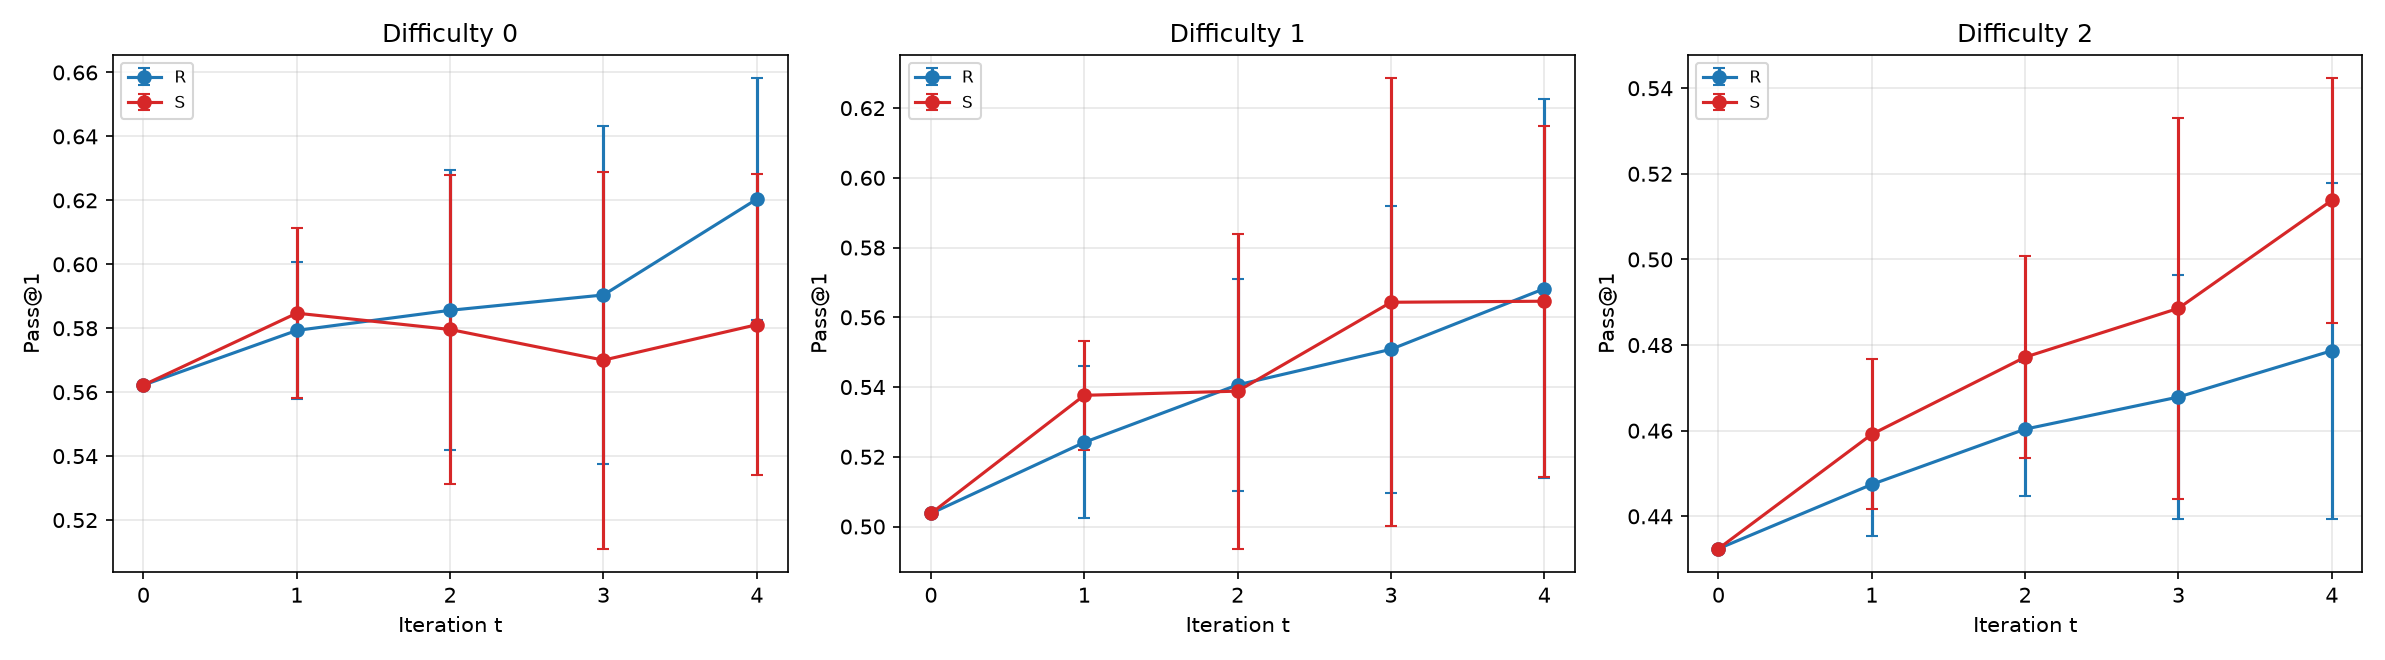
\includegraphics[width=0.90\linewidth]{figures/qwen_four_round_raw/unaudited_eval_id_by_difficulty.png}
\par\smallskip
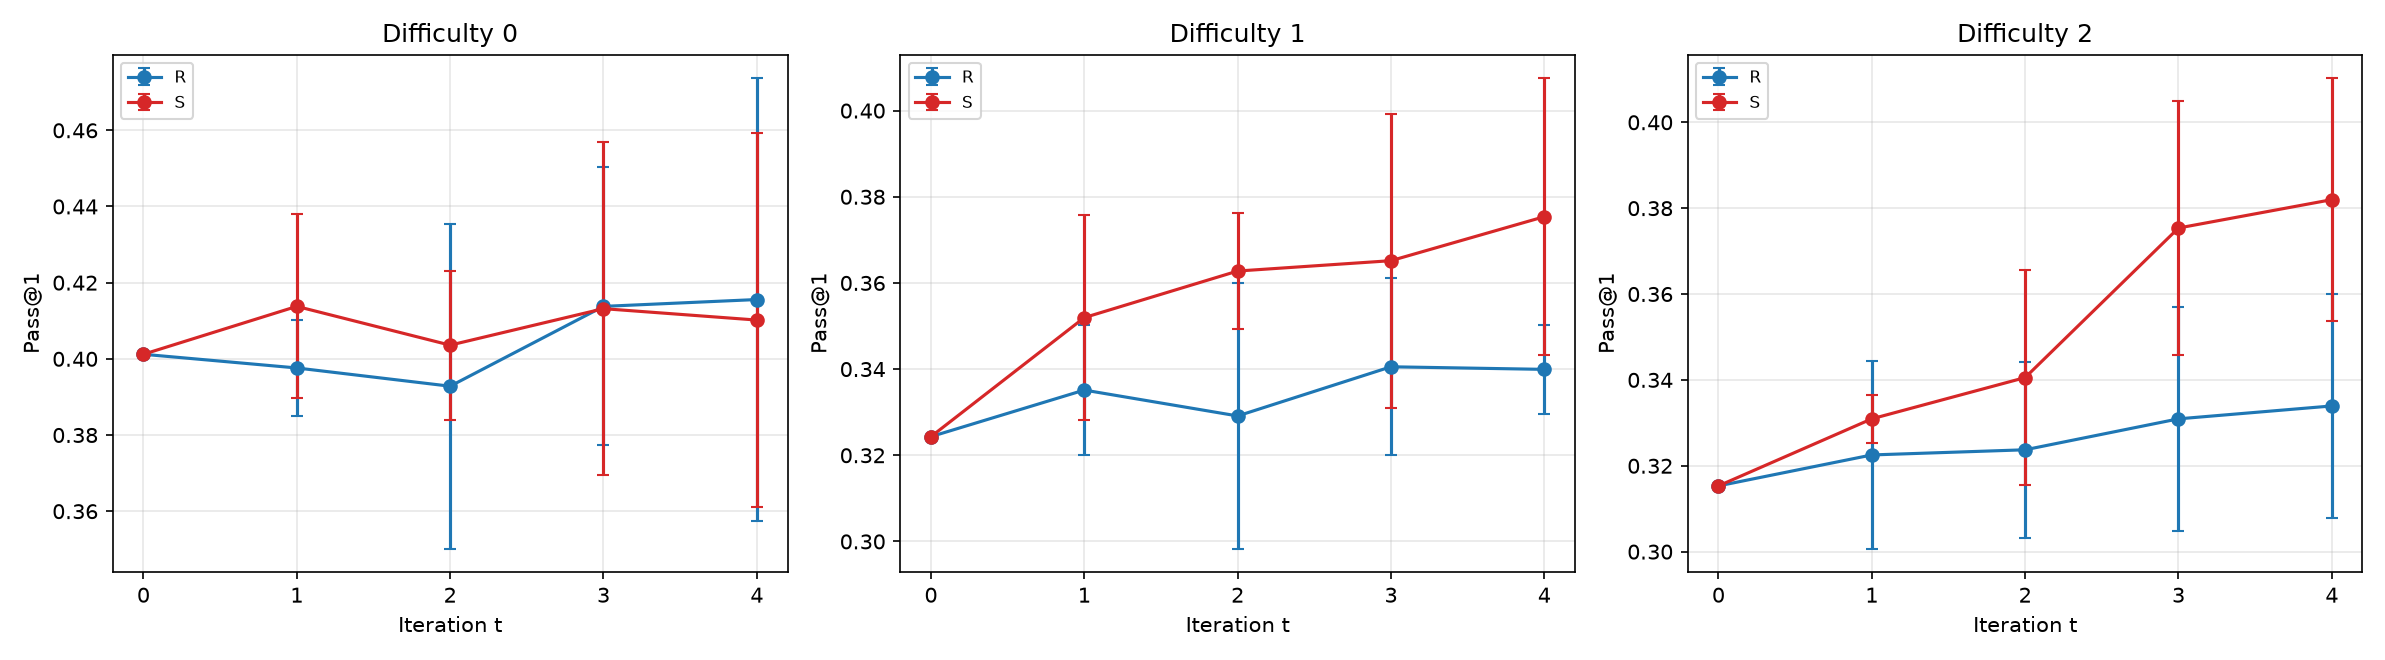
\includegraphics[width=0.90\linewidth]{figures/qwen_four_round_raw/unaudited_eval_ood_by_difficulty.png}
\caption{Original unaudited Qwen3-1.7B graph accuracy by generator
difficulty stratum, ID (top) and OOD (bottom), for rounds 0--4.
Strata 0--2 run from left to right and contain $667/667/666$ ID
and $334/333/333$ OOD questions. Error bars use the same five blocks
as Figure~\ref{fig:qwen-raw-unaudited}.}
\label{fig:qwen-raw-unaudited-difficulty}
\end{figure}

The strata are fixed features of the task generator, not an empirically
established ordering of model difficulty. Their separate vertical scales
are retained, so visual differences in slope do not by themselves
establish different learning rates. These descriptive trajectories
support no additional difficulty-specific significance claim.

\begin{figure}[H]
\centering
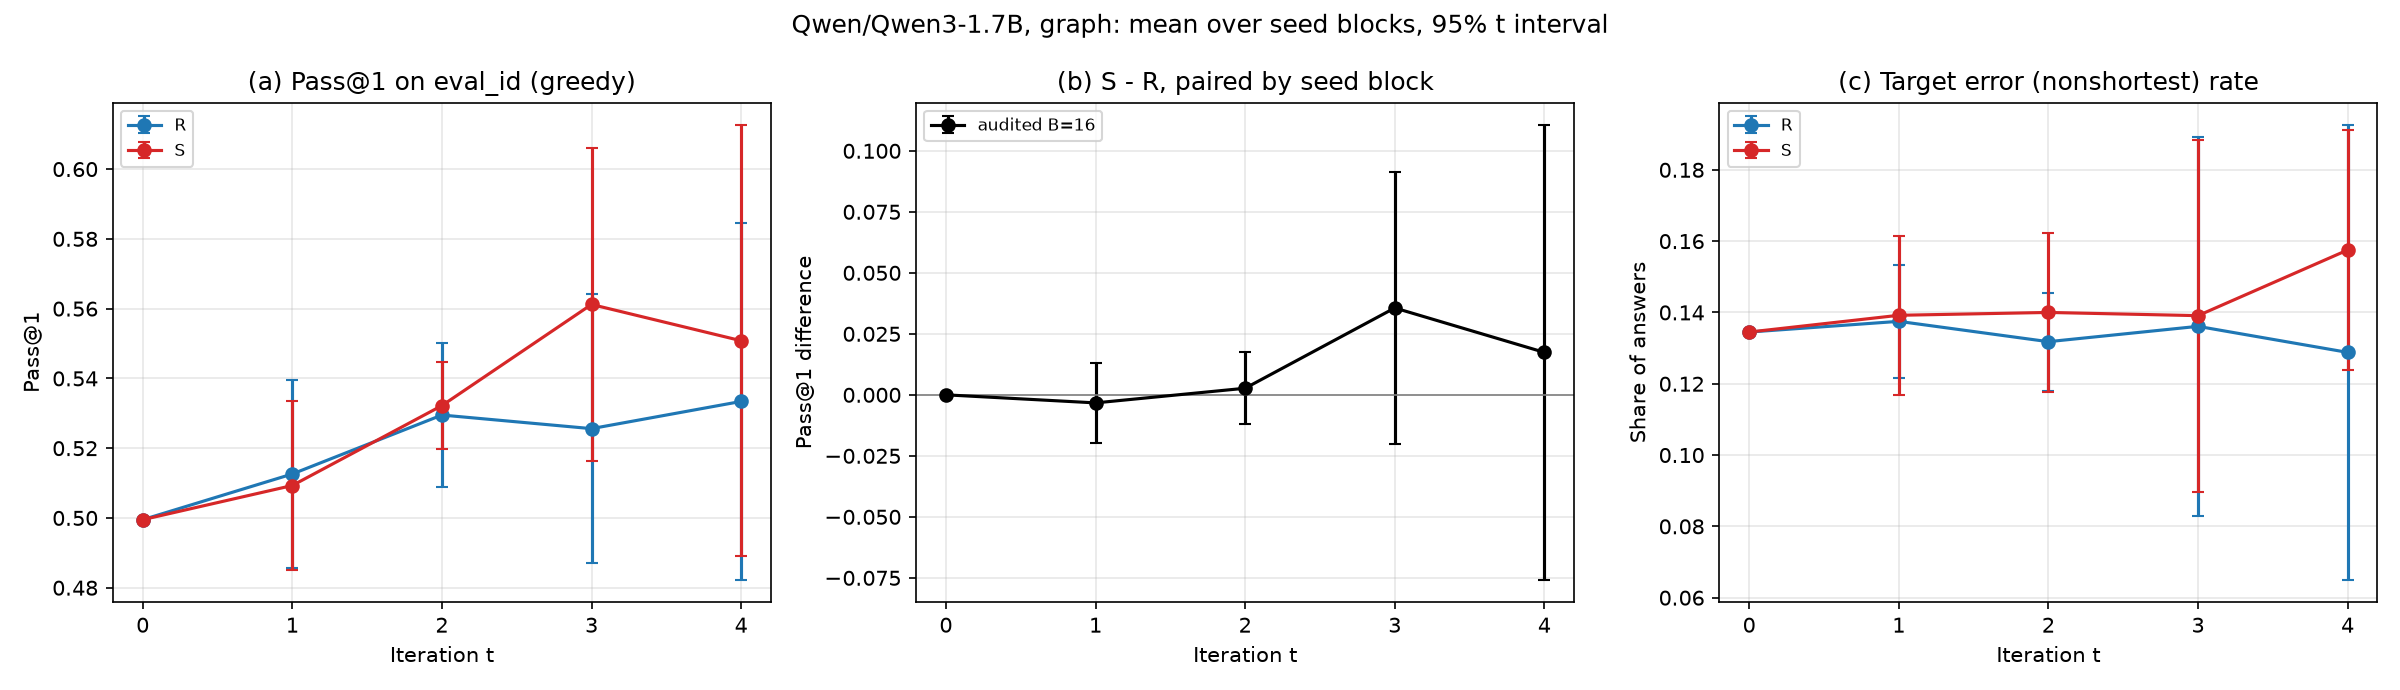
\includegraphics[width=0.90\linewidth]{figures/qwen_four_round_raw/audited_eval_id_pass1.png}
\par\smallskip
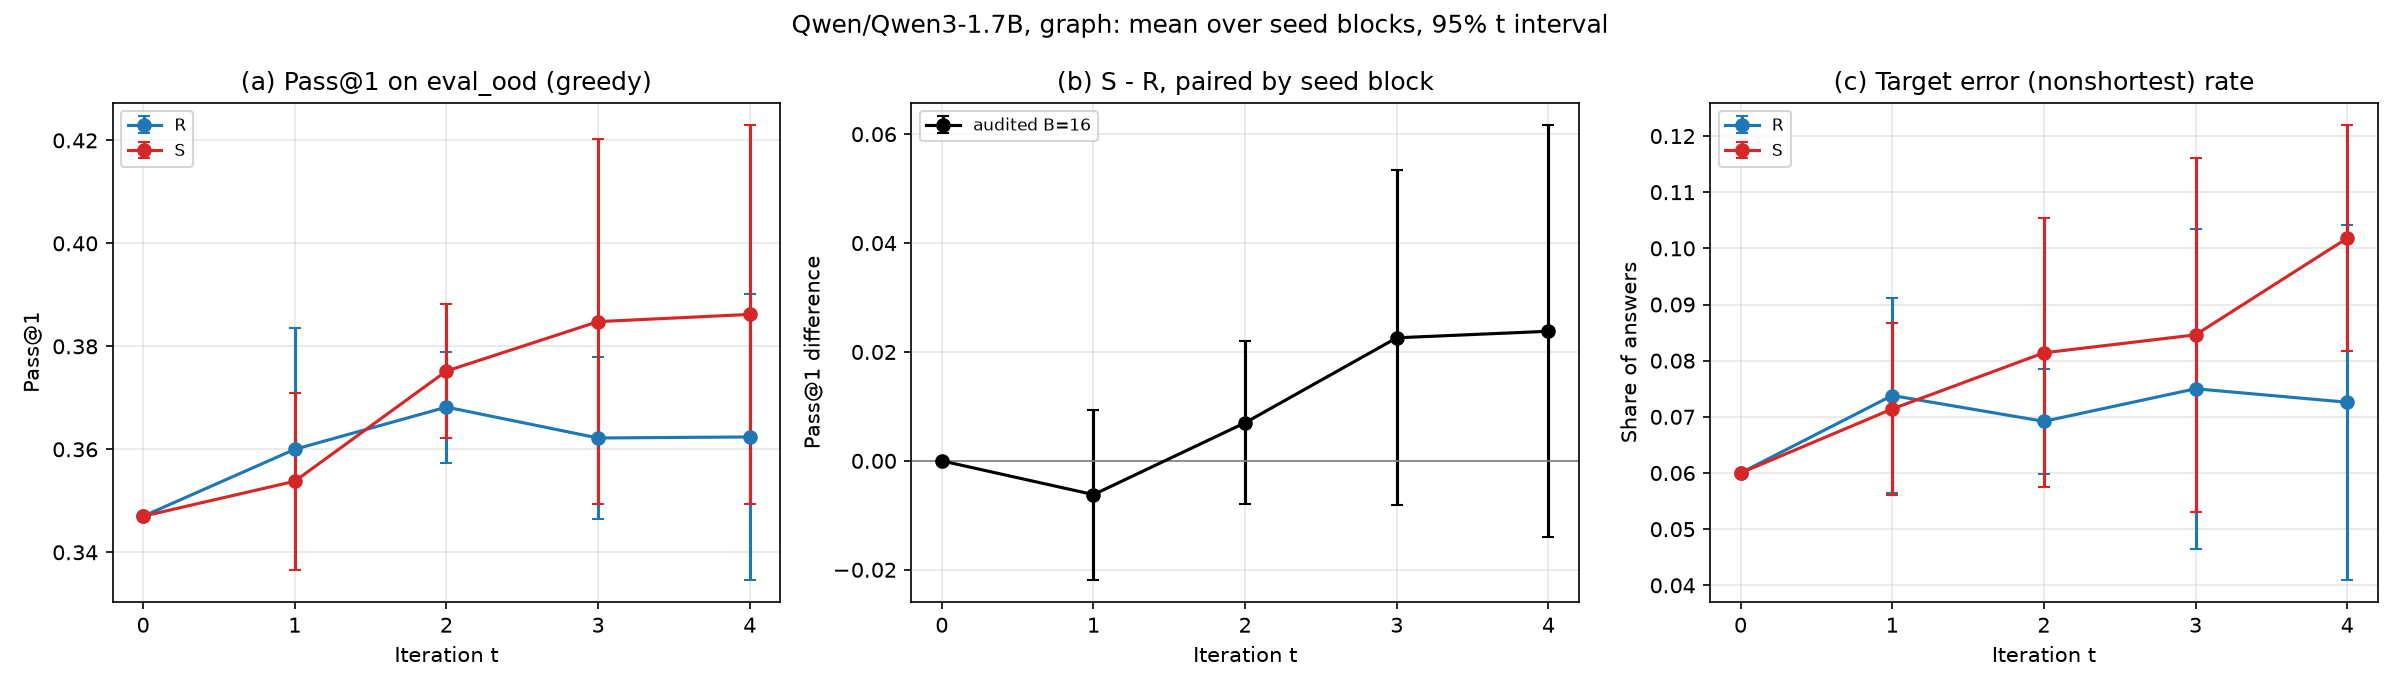
\includegraphics[width=0.90\linewidth]{figures/qwen_four_round_raw/audited_eval_ood_pass1.png}
\caption{Original adaptive-audit Qwen3-1.7B graph curves, ID (top)
and OOD (bottom), with $B_{\rm qry}=16$ correctness queries per
arm-round. The panels show greedy Pass@1, paired $S-R$ accuracy,
and nonshortest-error incidence. Each audited arm spends 64 queries
over four rounds.}
\label{fig:qwen-raw-audited}
\end{figure}

Under auditing, round-four $R/S$ accuracy is $0.533/0.551$ ID and
$0.362/0.386$ OOD. The paired contrasts are $0.017\pm0.093$ and
$0.024\pm0.038$, respectively. These contrasts
compare selection arms within the audited policy; they do not measure
the effect of adding an audit to an otherwise fixed training procedure.

\begin{figure}[H]
\centering
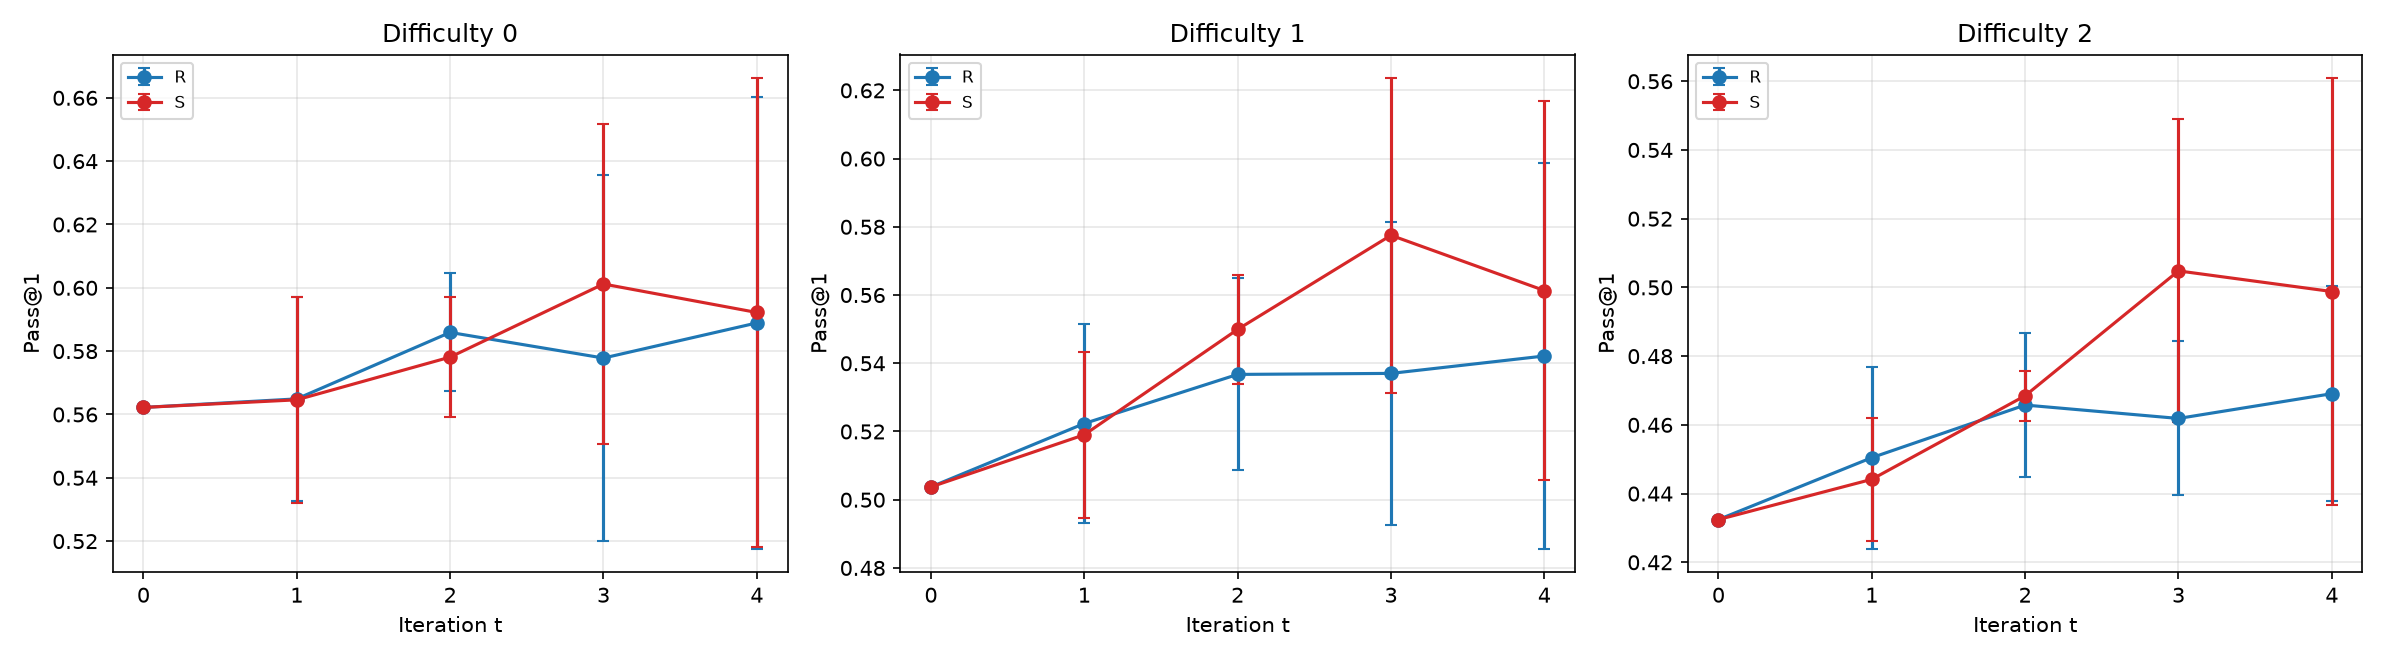
\includegraphics[width=0.90\linewidth]{figures/qwen_four_round_raw/audited_eval_id_by_difficulty.png}
\par\smallskip
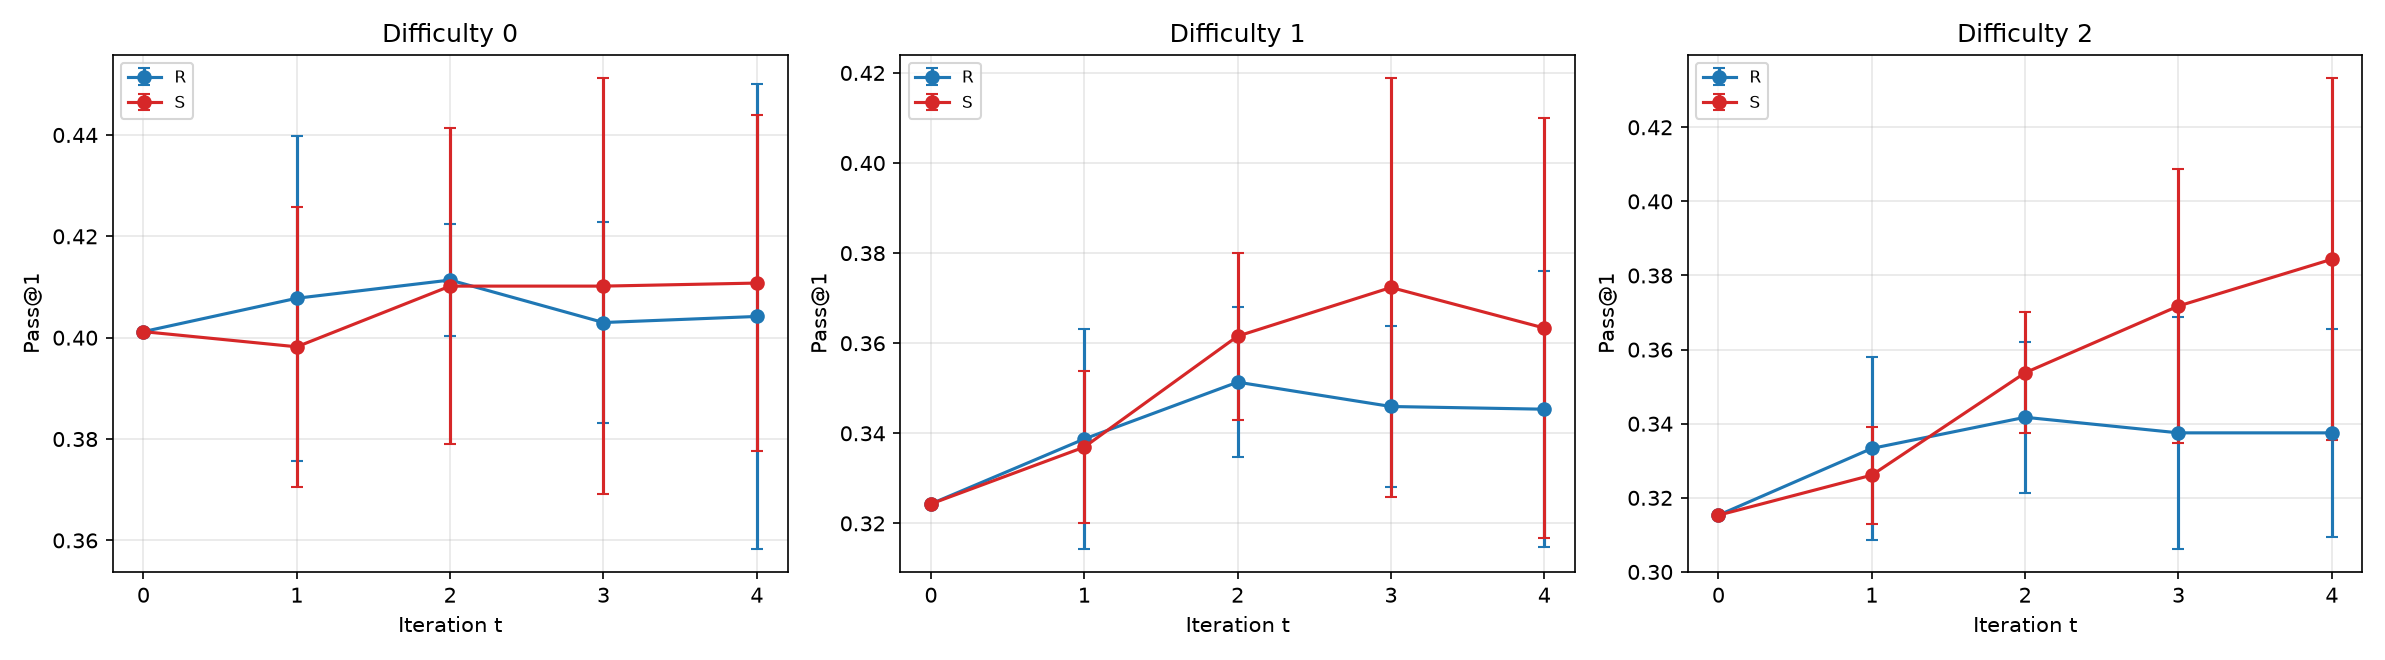
\includegraphics[width=0.90\linewidth]{figures/qwen_four_round_raw/audited_eval_ood_by_difficulty.png}
\caption{Original adaptive-audit Qwen3-1.7B graph accuracy by
generator stratum, ID (top) and OOD (bottom), for rounds 0--4.
The strata, fixed question sets, and pointwise block-$t$ intervals
follow Figure~\ref{fig:qwen-raw-unaudited-difficulty}.}
\label{fig:qwen-raw-audited-difficulty}
\end{figure}

The audited stratum curves supplement the aggregate results but do not
establish a stratum-specific audit benefit. They use the same fixed
questions as the unaudited curves, while retaining their original
separate vertical scales and pointwise uncertainty intervals.

\begin{figure}[H]
\centering
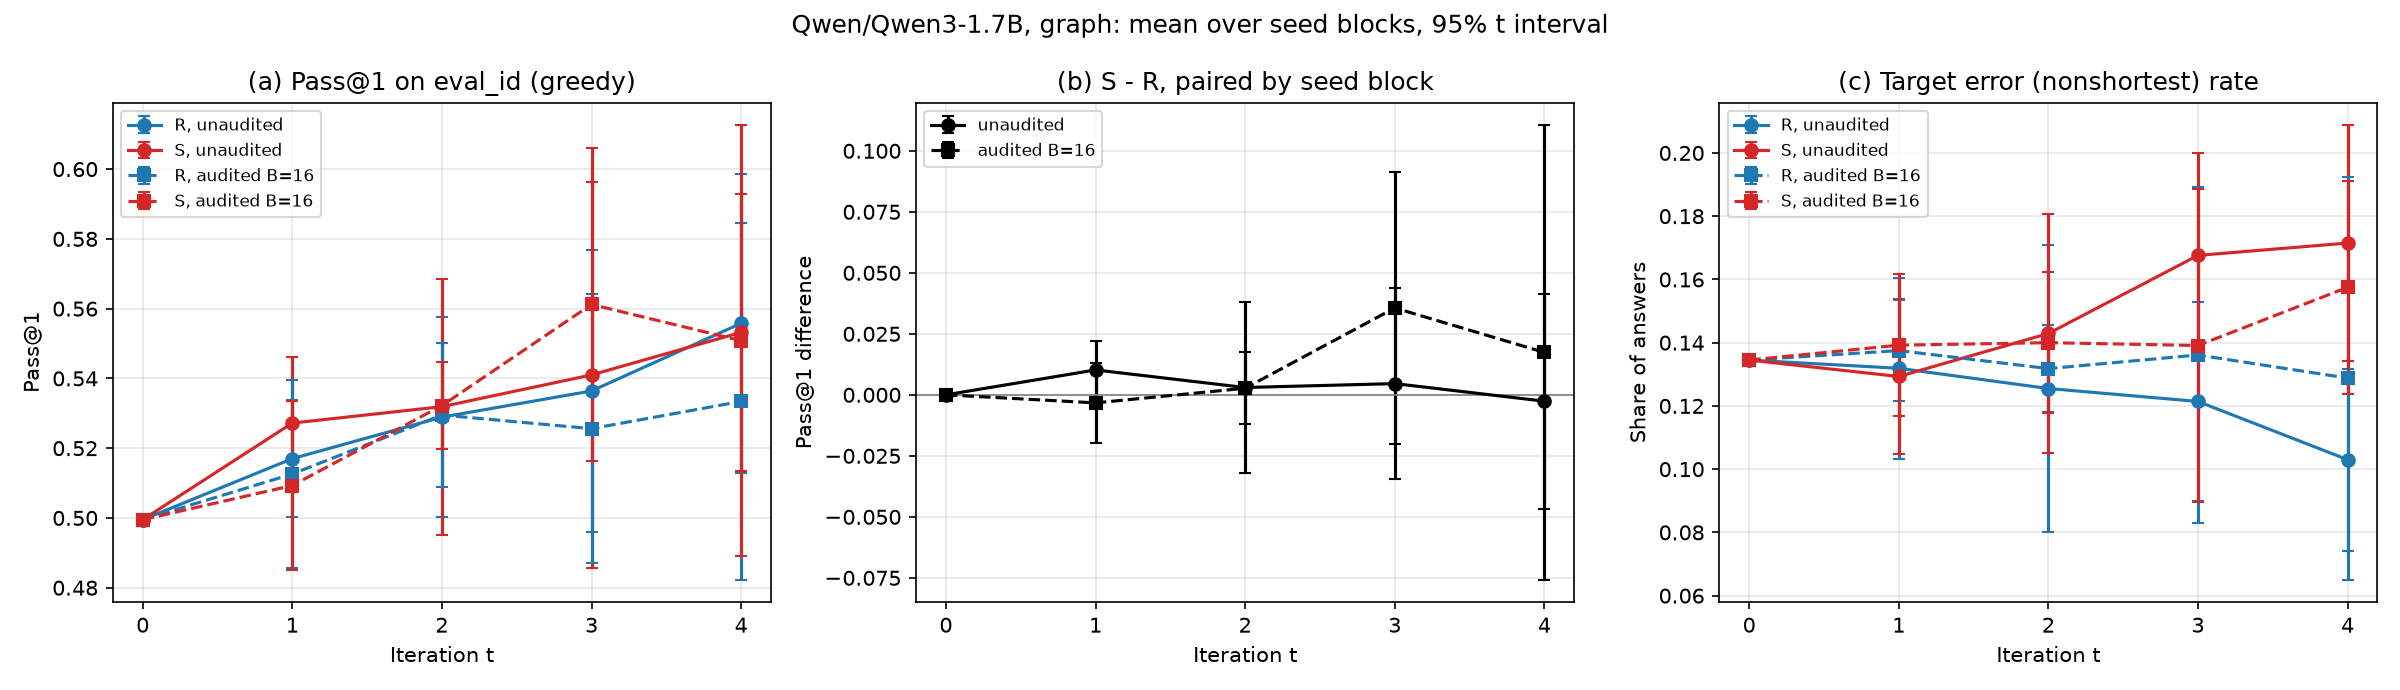
\includegraphics[width=0.90\linewidth]{figures/qwen_four_round_raw/comparison_eval_id_pass1.png}
\par\smallskip
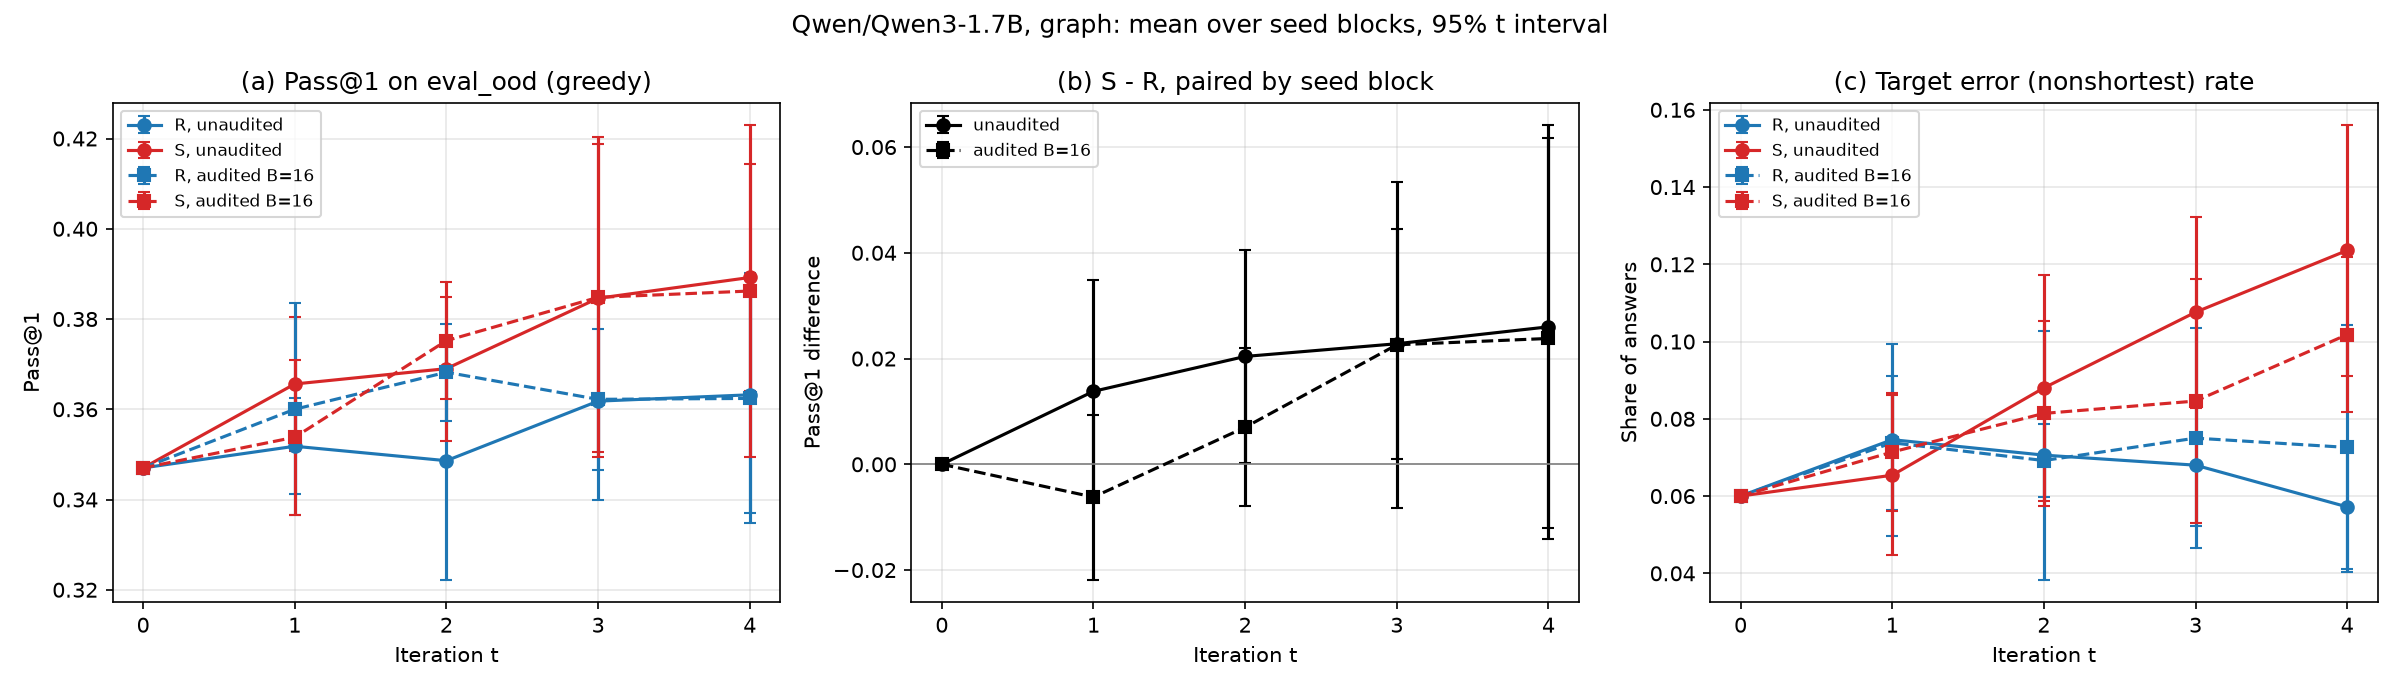
\includegraphics[width=0.90\linewidth]{figures/qwen_four_round_raw/comparison_eval_ood_pass1.png}
\caption{Original joint comparison of unaudited and adaptive-audit
Qwen3-1.7B graph trajectories, ID (top) and OOD (bottom), for
rounds 0--4. Each middle panel reports paired $S-R$ accuracy
separately within the two policies, not the effect of auditing.}
\label{fig:qwen-raw-comparison}
\end{figure}

Same-arm audited-minus-unaudited accuracy changes are negative in mean
(Table~\ref{tab:qwen-audit-change}).
The joint view therefore does not establish a uniform audit benefit;
it distinguishes within-policy arm differences from cross-policy changes.

\begin{figure}[H]
\centering
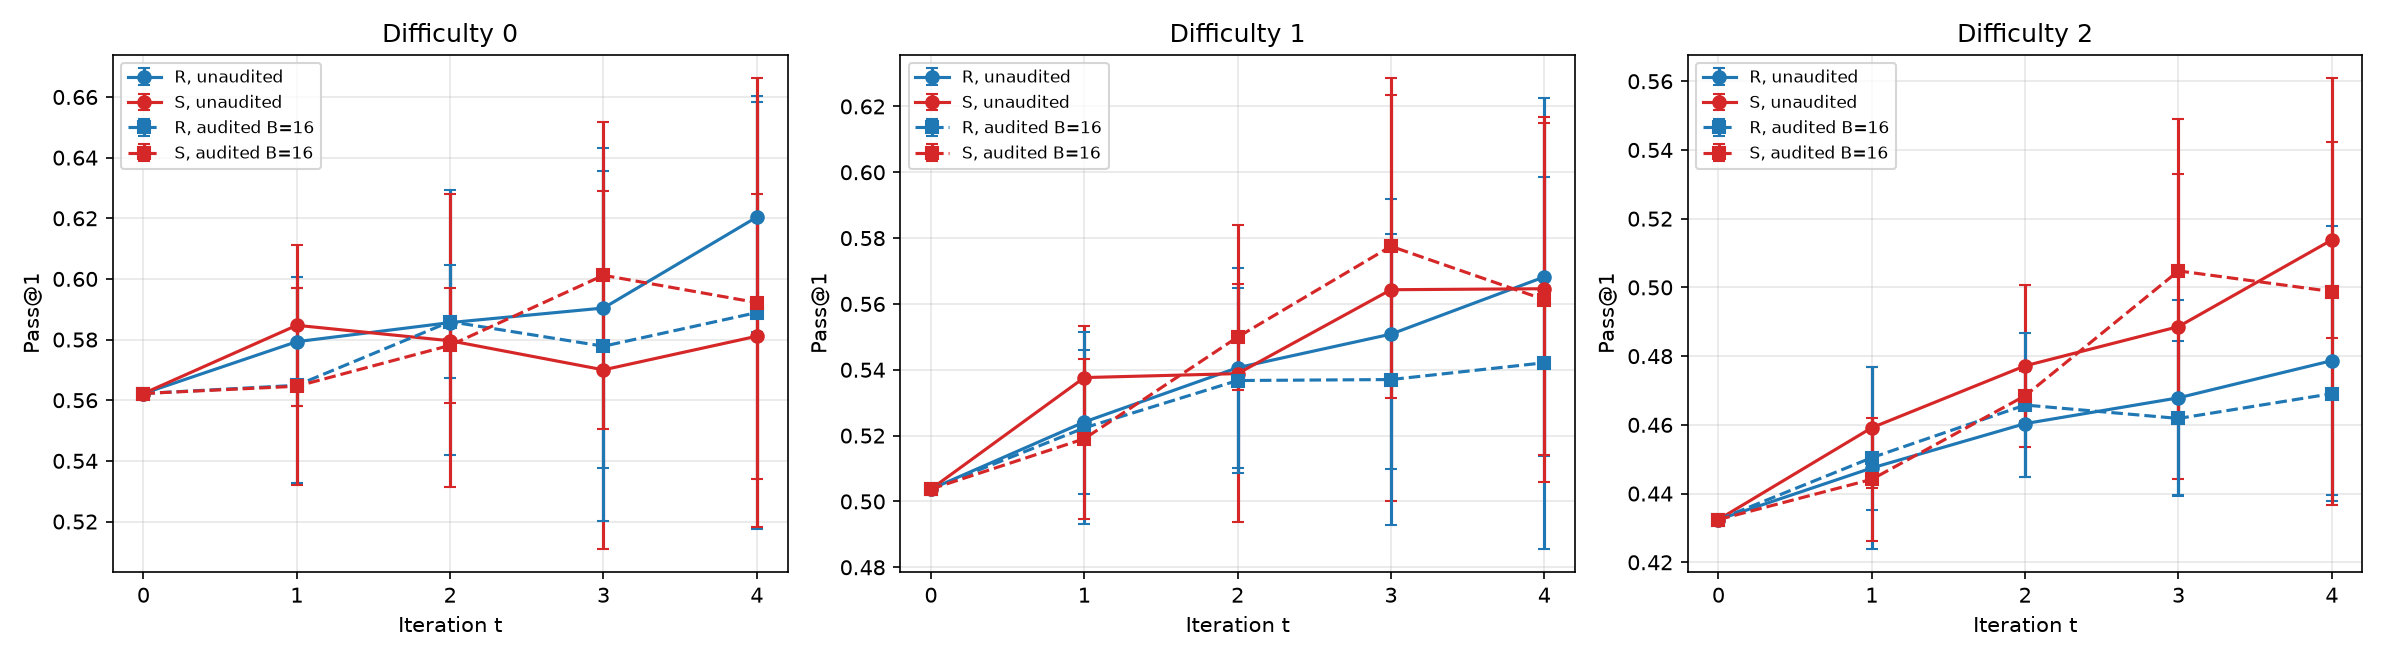
\includegraphics[width=0.90\linewidth]{figures/qwen_four_round_raw/comparison_eval_id_by_difficulty.png}
\par\smallskip
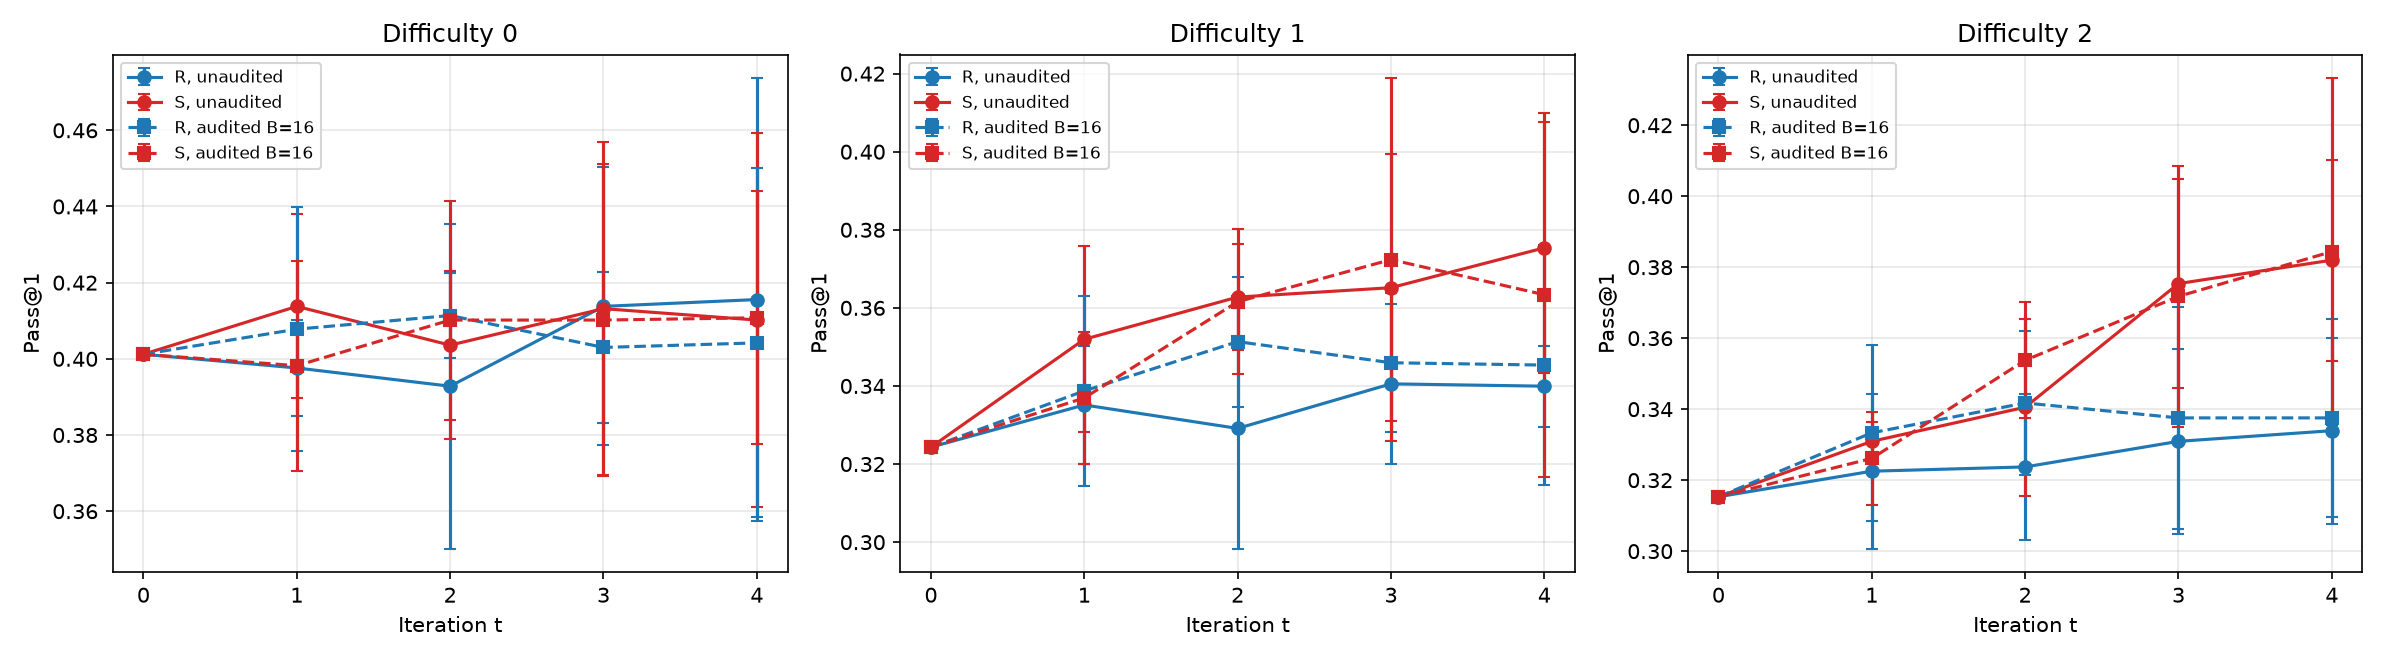
\includegraphics[width=0.90\linewidth]{figures/qwen_four_round_raw/comparison_eval_ood_by_difficulty.png}
\caption{Original joint Qwen3-1.7B graph accuracy curves by
generator stratum, ID (top) and OOD (bottom), for rounds 0--4.
Both policies and both arms use the same question stratum at
each checkpoint. Counts and interval conventions follow
Figure~\ref{fig:qwen-raw-unaudited-difficulty}.}
\label{fig:qwen-raw-comparison-difficulty}
\end{figure}

Both policies and both arms are evaluated on the same question stratum
at each checkpoint. Panel-specific vertical scales remain unchanged,
and the intervals are not adjusted for comparisons across strata,
rounds, or policies. The joint breakdown is consequently descriptive,
rather than a collection of confirmatory stratum-level tests.
\endgroup


\paragraph{Eight-round extension.}
The Llama-3.2-3B and Qwen3-1.7B trajectories continue to eight rounds.
Table~\ref{tab:eight-round-contrasts} reports the later paired accuracy
contrasts while retaining round four as the primary endpoint.
The unaudited Qwen3-1.7B OOD contrast favors $S$; these secondary
comparisons are descriptive and are not adjusted for multiplicity.
\begin{table}[H]
\caption{Round-eight graph accuracy contrasts $S-R$ (mean $\pm$ descriptive 95\% paired block-$t$ half-width over five blocks). Positive values favor $S$. ID and OOD evaluations use 2,000 and 1,000 fixed questions, respectively. These secondary endpoints supplement the primary four-round analysis.}
\label{tab:eight-round-contrasts}
\centering\small
\begin{tabular}{@{}llcc@{}}
\toprule
Model & Policy & ID Pass@1 $S-R$ & OOD Pass@1 $S-R$\\
\midrule
Llama-3.2-3B & Unaudited & $-0.029\pm0.111$ & $0.024\pm0.064$\\
Llama-3.2-3B & Adaptive, $B=16$ & $-0.031\pm0.086$ & $0.015\pm0.081$\\
Qwen3-1.7B & Unaudited & $0.040\pm0.045$ & $0.047\pm0.042$\\
Qwen3-1.7B & Adaptive, $B=16$ & $0.029\pm0.091$ & $0.037\pm0.063$\\
\bottomrule
\end{tabular}
\end{table}


\subsection{Qwen3-4B: four-round graph comparisons}
\label{app:qwen4b-four-round}

Both Qwen3-4B policies comprise five paired blocks and four rounds,
evaluated greedily on 2,000 ID and 1,000 OOD questions.
Table~\ref{tab:qwen4b-endpoints} reports endpoint accuracy and target incidence.
Unaudited OOD accuracy contrasts
at rounds two and three are $0.0308\pm0.0243$ and $0.0388\pm0.0233$,
but this intermediate advantage does not persist at round four.
These comparisons are not adjusted for multiplicity and do not constitute
a best-checkpoint analysis.

\begin{table}[H]
\caption{Qwen3-4B round-one matching, shared across both four-round policies and the one-step reuse. $N^+/N^-$ exclude truncated answers. Both arms have identical prompt and correct-response IDs, 48/16 correct/error quotas, and exact per-prompt supervised response lengths. Later checkpoint-dependent pools are not jointly matched.}
\label{tab:qwen4b-matching}
\centering\small\setlength{\tabcolsep}{3pt}
\begin{tabular}{@{}lllllll@{}}
\toprule
Block & $N^+/N^-$ & Cut & TPR/FPR & Yield & Target hits $R/S$ & Controls\\
\midrule
b00 & 10326/6049 & 9 & 0.004648/0.002645 & 0.003908 & 10/16 & pass\\
b01 & 10323/6054 & 7 & 0.004650/0.002643 & 0.003908 & 10/16 & pass\\
b02 & 10360/6014 & 10 & 0.004633/0.002660 & 0.003909 & 9/16 & pass\\
b03 & 10370/6009 & 5 & 0.004629/0.002663 & 0.003907 & 9/16 & pass\\
b04 & 10325/6050 & 9 & 0.004649/0.002645 & 0.003908 & 9/16 & pass\\
\bottomrule
\end{tabular}
\end{table}

\begin{table}[H]
\caption{Qwen3-4B graph endpoints after four rounds. Target rates count nonshortest answers among all evaluated questions. Paired $S-R$ differences are within policy, with descriptive 95\% block-$t$ half-widths over five blocks. Same-arm audit-change intervals appear in Table~\ref{tab:audit-results}.}
\label{tab:qwen4b-endpoints}
\centering\small\setlength{\tabcolsep}{3pt}
\begin{tabular}{@{}lllllll@{}}
\toprule
Split & Policy & Base & Pass@1 $R/S$ & $S-R$ Pass@1 & Target $R/S$ & $S-R$ target\\
\midrule
ID & None & 0.6125 & 0.7309/0.7339 & $0.0030\pm0.0968$ & 0.1026/0.1491 & $0.0465\pm0.1489$\\
ID & B=16 & 0.6100 & 0.7180/0.7273 & $0.0093\pm0.0745$ & 0.1375/0.1614 & $0.0239\pm0.0328$\\
OOD & None & 0.3970 & 0.4988/0.4982 & $-0.0006\pm0.0991$ & 0.1618/0.2644 & $0.1026\pm0.2015$\\
OOD & B=16 & 0.3960 & 0.4750/0.4850 & $0.0100\pm0.0741$ & 0.2060/0.2424 & $0.0364\pm0.0528$\\
\bottomrule
\end{tabular}
\end{table}


The identical round-one certificates confirm shared prompt/correct-response IDs,
$48/16$ correct/error counts, and exact response-token matching.
$R$ selects 9--10 nonshortest errors, versus 16 in $S$.
Audited training rows and weights agree with the reported
selection counts and effective sample sizes. Later pools are not jointly rate-matched.
Generation uses temperature $1.3$, top-$p=1$, and a mixed stopping schedule: block
\texttt{b00} uses no repetition stop throughout; \texttt{b01} introduces
it at round four, and \texttt{b02}--\texttt{b04} use it in later-round
generation throughout. The two arms share each block-round setting.
Their imported round-one pools were generated without this stop rule.
Thus the study is not a replication under one uniform generation profile.

Both policies improve in mean.
Same-arm audit error changes are positive in mean
(Table~\ref{tab:audit-results}). Each audited arm spends 64
queries per block, averaging 54.4/55.0 $R/S$ updates versus 64 unaudited.
These descriptive contrasts combine changes in data, weighting,
and optimizer effort.

Tables~\ref{tab:qwen4b-rounds} and~\ref{tab:qwen4b-blocks} report all four
rounds and all five endpoint blocks, rather than a selected checkpoint.
Table~\ref{tab:qwen4b-audit-change} gives accuracy changes with their
paired intervals, complementing the error changes in
Table~\ref{tab:audit-results}. Table~\ref{tab:qwen4b-audit} reports each
round's projection, retained volume, positive-weight coverage, ESS, and
TPRs. Retained-row TPR equals pre-audit TPR because audit deletion
preserves all 48 correct rows; positive-weight TPR can be smaller.
Rates use each round's original nontruncated-pool denominator and are
averages of block-level ratios, not ratios of pooled counts.
Table~\ref{tab:qwen4b-training} complements these readouts with per-round
parameter-change norms and training losses for the completed comparisons.
These quantities describe the training objective, not held-out accuracy;
losses under different weighting policies are not directly comparable.

\begin{table}[H]
\caption{Qwen3-4B four-round graph trajectories: means $\pm$ pointwise descriptive 95\% block-$t$ half-widths over five blocks. Target incidence counts nonshortest answers among all evaluated questions.}
\label{tab:qwen4b-rounds}
\centering\small\setlength{\tabcolsep}{3pt}
\begin{tabular}{@{}lllllllll@{}}
\toprule
Split & Policy & Round & Pass@1 $R$ & Pass@1 $S$ & Pass@1 $S-R$ & Target $R$ & Target $S$ & Target $S-R$\\
\midrule
ID & Base, none & 0 & 0.613 & 0.613 & --- & 0.215 & 0.215 & ---\\
ID & None & 1 & $0.614\pm0.032$ & $0.607\pm0.012$ & $-0.007\pm0.028$ & $0.215\pm0.029$ & $0.230\pm0.011$ & $0.015\pm0.030$\\
ID & None & 2 & $0.634\pm0.033$ & $0.650\pm0.034$ & $0.016\pm0.034$ & $0.196\pm0.035$ & $0.190\pm0.042$ & $-0.007\pm0.046$\\
ID & None & 3 & $0.680\pm0.022$ & $0.703\pm0.030$ & $0.023\pm0.039$ & $0.138\pm0.053$ & $0.155\pm0.053$ & $0.017\pm0.090$\\
ID & None & 4 & $0.731\pm0.056$ & $0.734\pm0.067$ & $0.003\pm0.097$ & $0.103\pm0.094$ & $0.149\pm0.076$ & $0.046\pm0.149$\\
ID & Base, B=16 & 0 & 0.610 & 0.610 & --- & 0.220 & 0.220 & ---\\
ID & B=16 & 1 & $0.622\pm0.025$ & $0.622\pm0.044$ & $0.000\pm0.036$ & $0.205\pm0.016$ & $0.213\pm0.048$ & $0.007\pm0.047$\\
ID & B=16 & 2 & $0.654\pm0.040$ & $0.663\pm0.071$ & $0.009\pm0.062$ & $0.179\pm0.047$ & $0.177\pm0.071$ & $-0.003\pm0.092$\\
ID & B=16 & 3 & $0.698\pm0.042$ & $0.714\pm0.084$ & $0.016\pm0.060$ & $0.143\pm0.042$ & $0.143\pm0.078$ & $-0.000\pm0.065$\\
ID & B=16 & 4 & $0.718\pm0.068$ & $0.727\pm0.072$ & $0.009\pm0.075$ & $0.138\pm0.068$ & $0.161\pm0.054$ & $0.024\pm0.033$\\
OOD & Base, none & 0 & 0.397 & 0.397 & --- & 0.260 & 0.260 & ---\\
OOD & None & 1 & $0.394\pm0.014$ & $0.392\pm0.011$ & $-0.002\pm0.022$ & $0.258\pm0.016$ & $0.285\pm0.018$ & $0.027\pm0.022$\\
OOD & None & 2 & $0.398\pm0.023$ & $0.429\pm0.027$ & $0.031\pm0.024$ & $0.250\pm0.029$ & $0.257\pm0.038$ & $0.006\pm0.046$\\
OOD & None & 3 & $0.432\pm0.019$ & $0.471\pm0.025$ & $0.039\pm0.023$ & $0.191\pm0.074$ & $0.253\pm0.047$ & $0.062\pm0.098$\\
OOD & None & 4 & $0.499\pm0.049$ & $0.498\pm0.062$ & $-0.001\pm0.099$ & $0.162\pm0.129$ & $0.264\pm0.084$ & $0.103\pm0.202$\\
OOD & Base, B=16 & 0 & 0.396 & 0.396 & --- & 0.260 & 0.260 & ---\\
OOD & B=16 & 1 & $0.399\pm0.031$ & $0.399\pm0.034$ & $-0.000\pm0.028$ & $0.246\pm0.010$ & $0.259\pm0.034$ & $0.013\pm0.040$\\
OOD & B=16 & 2 & $0.420\pm0.037$ & $0.429\pm0.058$ & $0.008\pm0.054$ & $0.236\pm0.048$ & $0.230\pm0.057$ & $-0.007\pm0.091$\\
OOD & B=16 & 3 & $0.459\pm0.029$ & $0.478\pm0.082$ & $0.019\pm0.064$ & $0.207\pm0.055$ & $0.205\pm0.066$ & $-0.002\pm0.076$\\
OOD & B=16 & 4 & $0.475\pm0.079$ & $0.485\pm0.048$ & $0.010\pm0.074$ & $0.206\pm0.058$ & $0.242\pm0.033$ & $0.036\pm0.053$\\
\bottomrule
\end{tabular}
\end{table}

\begin{table}[H]
\caption{Qwen3-4B round-four graph endpoints by paired block. Slash-separated entries are $R/S$ values, not ratios. All five blocks are retained, including unfavorable audit changes.}
\label{tab:qwen4b-blocks}
\centering\small\setlength{\tabcolsep}{3pt}
\begin{tabular}{@{}llllll@{}}
\toprule
Policy & Block & ID Pass@1 & OOD Pass@1 & ID target & OOD target\\
\midrule
None & b00 & 0.7115/0.6750 & 0.5030/0.4470 & 0.0325/0.1935 & 0.0480/0.3200\\
None & b01 & 0.6615/0.7710 & 0.4320/0.5490 & 0.2300/0.1100 & 0.3290/0.1910\\
None & b02 & 0.7740/0.6740 & 0.5340/0.4430 & 0.0690/0.2345 & 0.1190/0.3500\\
None & b03 & 0.7570/0.7700 & 0.5050/0.5150 & 0.1050/0.1055 & 0.1720/0.2280\\
None & b04 & 0.7505/0.7795 & 0.5200/0.5370 & 0.0765/0.1020 & 0.1410/0.2330\\
B=16 & b00 & 0.6295/0.7200 & 0.3920/0.4790 & 0.2045/0.1860 & 0.2290/0.2670\\
B=16 & b01 & 0.7250/0.7240 & 0.4420/0.4960 & 0.1205/0.1350 & 0.1920/0.1990\\
B=16 & b02 & 0.7520/0.7850 & 0.5250/0.5260 & 0.0940/0.1365 & 0.1670/0.2480\\
B=16 & b03 & 0.7115/0.6370 & 0.4650/0.4230 & 0.1855/0.2255 & 0.2760/0.2580\\
B=16 & b04 & 0.7720/0.7705 & 0.5510/0.5010 & 0.0830/0.1240 & 0.1660/0.2400\\
\bottomrule
\end{tabular}
\end{table}

\begin{table}[H]
\caption{Qwen3-4B same-arm audited-minus-unaudited accuracy changes at round four (positive favors auditing), with paired 95\% block-$t$ half-widths. Unaudited arms each take 64 steps; auditing also changes retained data, weights, and optimizer effort.}
\label{tab:qwen4b-audit-change}
\centering\small\setlength{\tabcolsep}{3pt}
\begin{tabular}{@{}lllll@{}}
\toprule
Arm & Queries & Audited steps: mean [range] & ID accuracy change & OOD accuracy change\\
\midrule
R & 64 & 54.4 [49--61] & $-0.0129\pm0.0706$ & $-0.0238\pm0.0687$\\
S & 64 & 55.0 [52--57] & $-0.0066\pm0.1147$ & $-0.0132\pm0.0869$\\
\bottomrule
\end{tabular}
\end{table}

\begin{table}[H]
\caption{Qwen3-4B graph update and audit readouts, means over five blocks. $K\prime$ counts retained rows, $n^+$ positive-weight rows, and ESS is verified from audited weights. TPRs are percentages on each round-specific original nontruncated pool: pre-audit $48/N^+$ and positive-weight correct count divided by $N^+$. All 48 correct rows survive deletion, so retained post-audit TPR equals pre-audit TPR. The projection uses the fixed initial reference gradient, not measured task risk.}
\label{tab:qwen4b-audit}
\centering\small\setlength{\tabcolsep}{3pt}
\begin{tabular}{@{}llllllllll@{}}
\toprule
Round & Policy & Arm & $h^T\Delta\theta_t$ & Steps & $K\prime$ & $n^+$ & ESS & Pre TPR (\%) & Positive TPR (\%)\\
\midrule
1 & None & R & $-0.1487$ & 16.0 & 64.0 & 64.0 & 64.00 & 0.4642 & 0.4642\\
1 & None & S & $-0.1479$ & 16.0 & 64.0 & 64.0 & 64.00 & 0.4642 & 0.4642\\
1 & B=16 & R & $-0.0707$ & 13.2 & 60.0 & 50.6 & 40.33 & 0.4642 & 0.3984\\
1 & B=16 & S & $-0.0918$ & 13.2 & 60.0 & 50.6 & 40.33 & 0.4642 & 0.3984\\
2 & None & R & $-0.0985$ & 16.0 & 64.0 & 64.0 & 64.00 & 0.4657 & 0.4657\\
2 & None & S & $-0.0902$ & 16.0 & 64.0 & 64.0 & 64.00 & 0.4733 & 0.4733\\
2 & B=16 & R & $-0.1181$ & 14.8 & 61.0 & 57.0 & 48.83 & 0.4589 & 0.4293\\
2 & B=16 & S & $-0.1208$ & 13.6 & 60.0 & 52.6 & 43.83 & 0.4663 & 0.4166\\
3 & None & R & $-0.0697$ & 16.0 & 64.0 & 64.0 & 64.00 & 0.5134 & 0.5134\\
3 & None & S & $-0.0651$ & 16.0 & 64.0 & 64.0 & 64.00 & 0.4895 & 0.4895\\
3 & B=16 & R & $-0.0819$ & 12.4 & 59.4 & 48.0 & 37.98 & 0.4684 & 0.3829\\
3 & B=16 & S & $-0.0836$ & 12.4 & 59.4 & 49.0 & 39.39 & 0.4698 & 0.3876\\
4 & None & R & $-0.0524$ & 16.0 & 64.0 & 64.0 & 64.00 & 0.5735 & 0.5735\\
4 & None & S & $-0.0323$ & 16.0 & 64.0 & 64.0 & 64.00 & 0.5305 & 0.5305\\
4 & B=16 & R & $-0.0444$ & 14.0 & 60.2 & 55.4 & 44.71 & 0.4523 & 0.4173\\
4 & B=16 & S & $-0.0488$ & 15.8 & 61.2 & 61.2 & 50.03 & 0.4546 & 0.4546\\
\bottomrule
\end{tabular}
\end{table}

\begin{table}[H]
\caption{Qwen3-4B four-round training diagnostics, means over five blocks per arm and policy. $\Delta\theta_t$ is the parameter change within round $t$; $h$ is fixed at initialization. Norms are not cumulative displacement norms, and loss is the policy-specific weighted training objective. Neither projection nor training loss is held-out task accuracy.}
\label{tab:qwen4b-training}
\centering\small\setlength{\tabcolsep}{4pt}
\begin{tabular}{@{}lllrrr@{}}
\toprule
Round & Audit & Arm & $h^T\Delta\theta_t$ & $\|\Delta\theta_t\|_2$ & Loss\\
\midrule
1 & None & R & $-0.1487$ & 1.5161 & 0.0309\\
1 & None & S & $-0.1479$ & 1.5474 & 0.0364\\
1 & B=16 & R & $-0.0707$ & 1.2888 & 0.0309\\
1 & B=16 & S & $-0.0918$ & 1.3315 & 0.0332\\
2 & None & R & $-0.0985$ & 1.6279 & 0.0415\\
2 & None & S & $-0.0902$ & 1.6084 & 0.0411\\
2 & B=16 & R & $-0.1181$ & 1.5290 & 0.0308\\
2 & B=16 & S & $-0.1208$ & 1.4442 & 0.0311\\
3 & None & R & $-0.0697$ & 1.5263 & 0.0714\\
3 & None & S & $-0.0651$ & 1.5377 & 0.0643\\
3 & B=16 & R & $-0.0819$ & 1.3484 & 0.0353\\
3 & B=16 & S & $-0.0836$ & 1.3693 & 0.0304\\
4 & None & R & $-0.0524$ & 1.5233 & 0.3888\\
4 & None & S & $-0.0323$ & 1.5071 & 0.0719\\
4 & B=16 & R & $-0.0444$ & 1.3811 & 0.0704\\
4 & B=16 & S & $-0.0488$ & 1.5224 & 0.0426\\
\bottomrule
\end{tabular}
\end{table}


\paragraph{Validation scope.}
Accuracy and target incidence are reconstructed from 82 checkpoint--split
count records per policy, with all 40 training completions per policy checked.
All 123,000 audited held-out responses are independently rejudged, including
truncated answers in the evaluation denominators. Audit queries, retained
volume, positive-weight counts, and ESS agree with the training records.
Unaudited validation remains count-based because answers are unavailable.
Audited checkpoints are not reloaded; missing shared initialization and
reference tensors preclude independent gradient recomputation.
The 81,920 shared round-one candidate responses are also independently
rejudged; eligible-pool counts agree with the matching certificates.
Exact-length eligibility is reported from those certificates rather than
independently retokenized.

\begin{figure}[H]
\centering
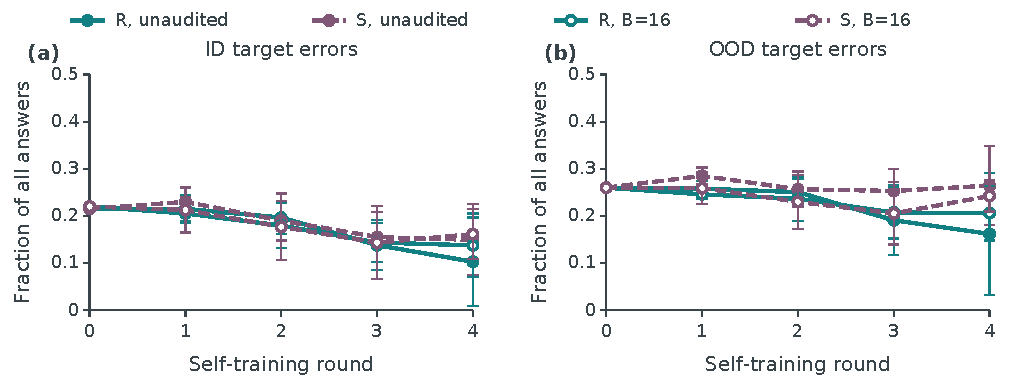
\includegraphics[width=0.8\linewidth]{figures/qwen4b_multiround/qwen4b_target_errors.pdf}
\caption{Qwen3-4B nonshortest-error incidence among all evaluated answers.
Unaudited $R/S$ endpoints are $0.1026/0.1491$ ID and $0.1618/0.2644$ OOD;
audited endpoints are $0.1375/0.1614$ and $0.2060/0.2424$.
Paired contrasts appear in Table~\ref{tab:qwen4b-endpoints}.
Bars are pointwise block-$t$ intervals
over five blocks.}
\label{fig:qwen4b-target-errors}
\end{figure}

\begingroup
\let\figure\RSIappendixfigure
\let\endfigure\RSIendappendixfigure
\subsubsection{Original four-round Qwen3-4B figures}
\label{app:qwen4b-raw-figures}

Figures~\ref{fig:qwen4b-raw-unaudited}--\ref{fig:qwen4b-raw-comparison-difficulty}
present the Qwen3-4B trajectories in the same six groups as
Appendix~\ref{app:qwen-raw-figures}: unaudited, audited, and joint
comparisons, each with aggregate and difficulty-stratified views.
The separate-policy plots are original exports; the joint views are
generated from the same checkpoint records with the same plotting method.
They complement Figure~\ref{fig:graph-four-round}(c--d) and
Table~\ref{tab:qwen4b-endpoints}, not additional experiments.
All use five paired blocks and fixed sets of 2,000 ID or 1,000 OOD
questions. Error bars are pointwise, descriptive 95\% block-$t$ intervals.

\begin{figure}[H]
\centering
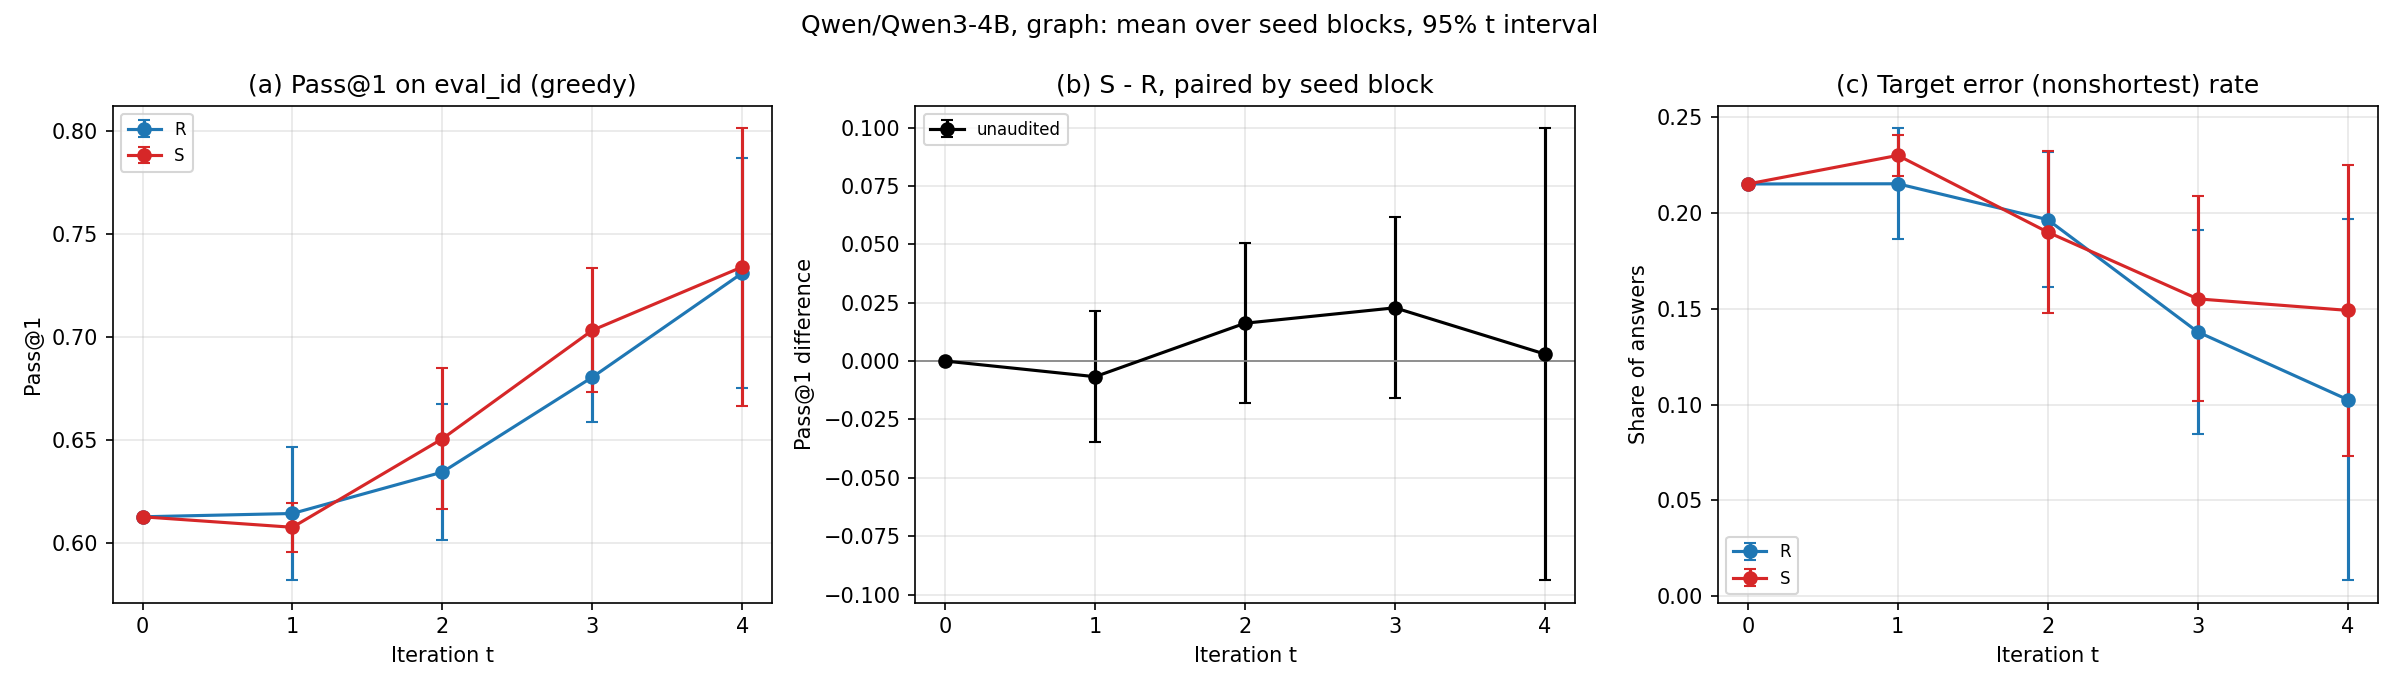
\includegraphics[width=0.90\linewidth]{figures/qwen4b_four_round_raw/unaudited_eval_id_pass1.png}
\par\smallskip
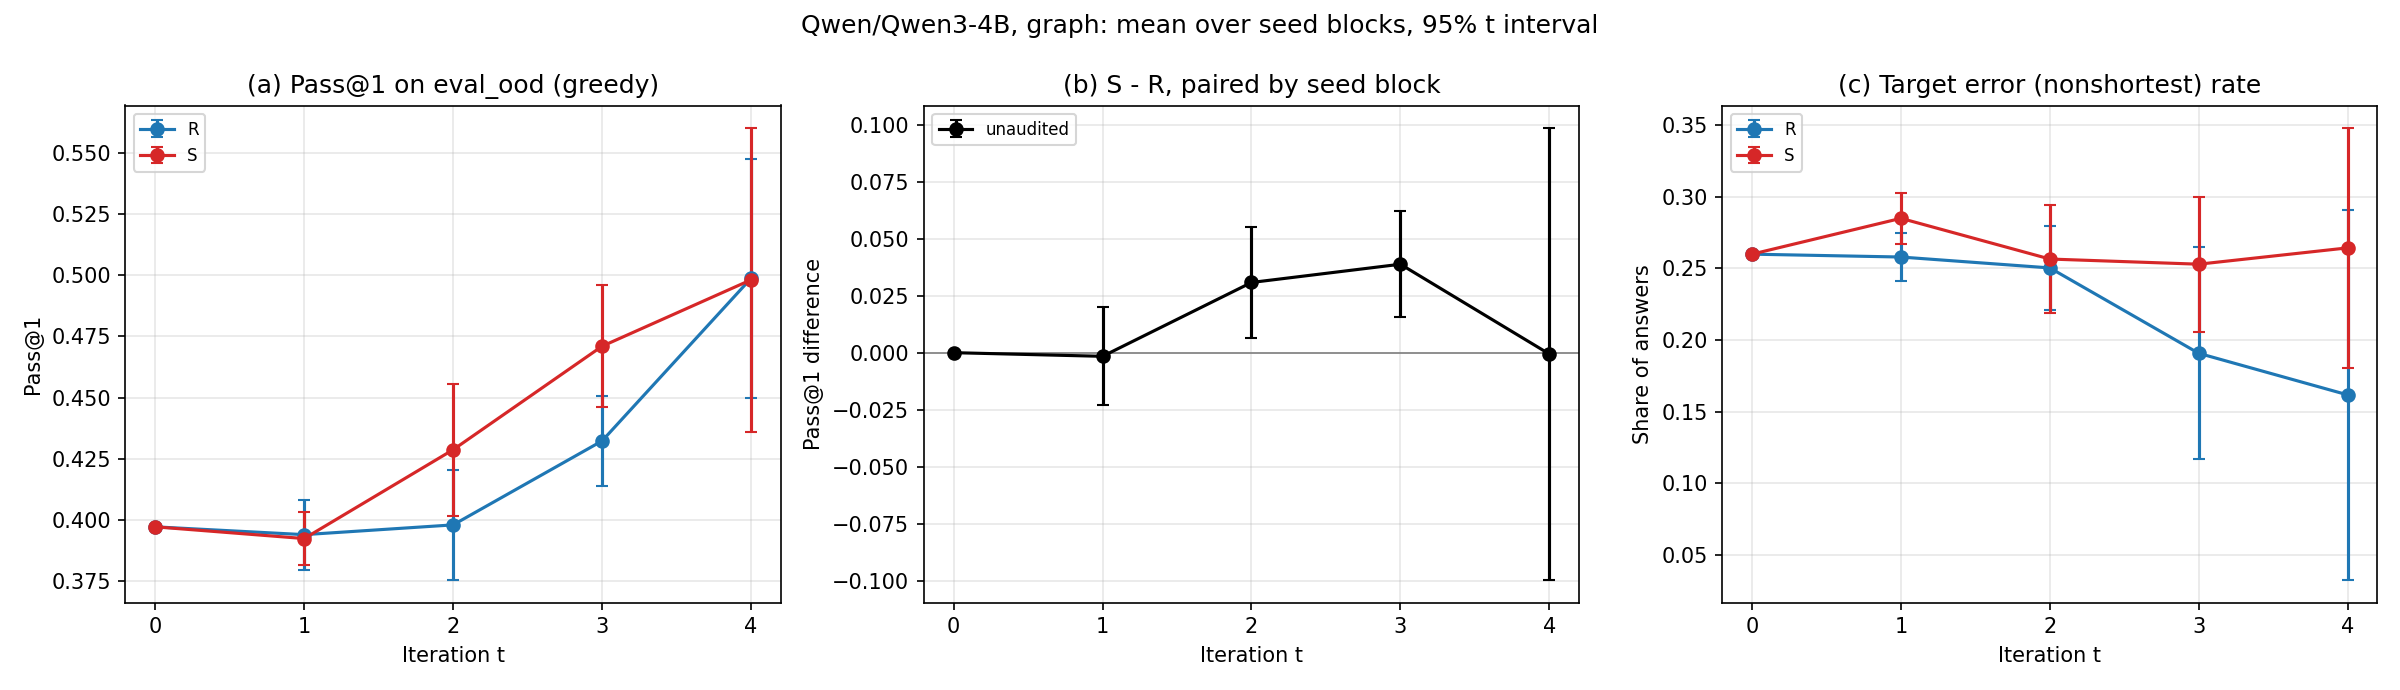
\includegraphics[width=0.90\linewidth]{figures/qwen4b_four_round_raw/unaudited_eval_ood_pass1.png}
\caption{Original unaudited Qwen3-4B graph curves, ID (top) and OOD
(bottom), for rounds 0--4. The panels show greedy Pass@1, paired
$S-R$ accuracy, and nonshortest-error incidence among all answers.}
\label{fig:qwen4b-raw-unaudited}
\end{figure}

Unaudited $R/S$ accuracy reaches $0.7309/0.7339$ ID and
$0.4988/0.4982$ OOD, from bases $0.6125$ and $0.3970$.
Paired endpoint contrasts are $0.0030\pm0.0968$ ID and
$-0.0006\pm0.0991$ OOD. The positive mean OOD contrast in
intermediate rounds declines to near zero at the endpoint.

\begin{figure}[H]
\centering
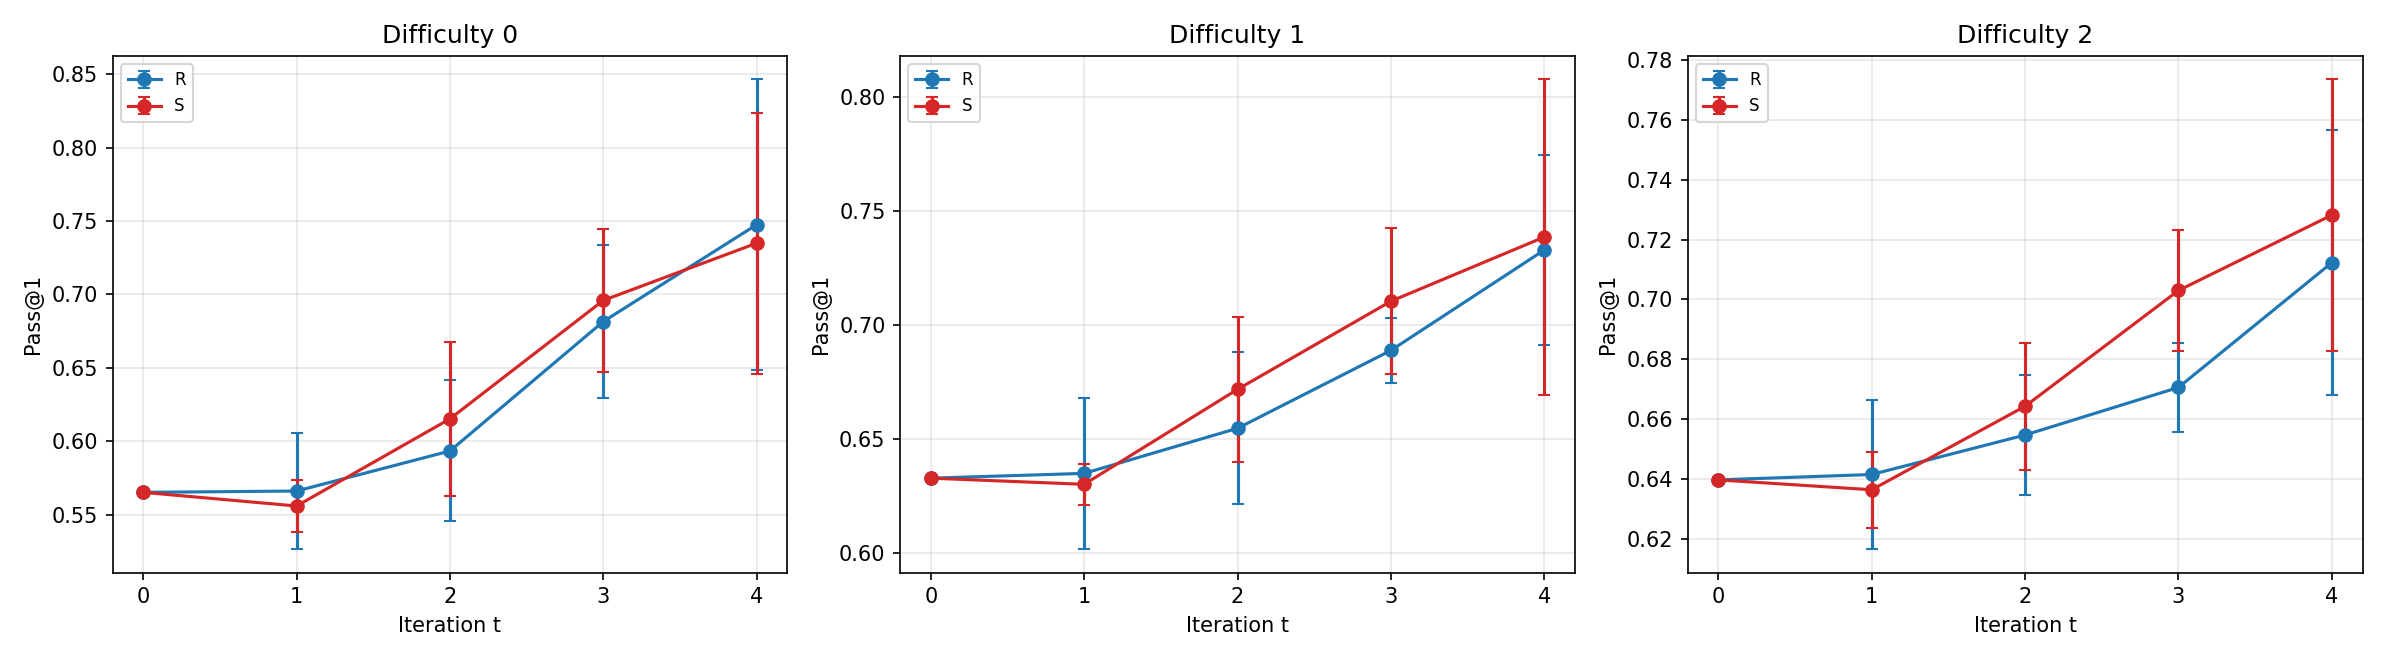
\includegraphics[width=0.90\linewidth]{figures/qwen4b_four_round_raw/unaudited_eval_id_by_difficulty.png}
\par\smallskip
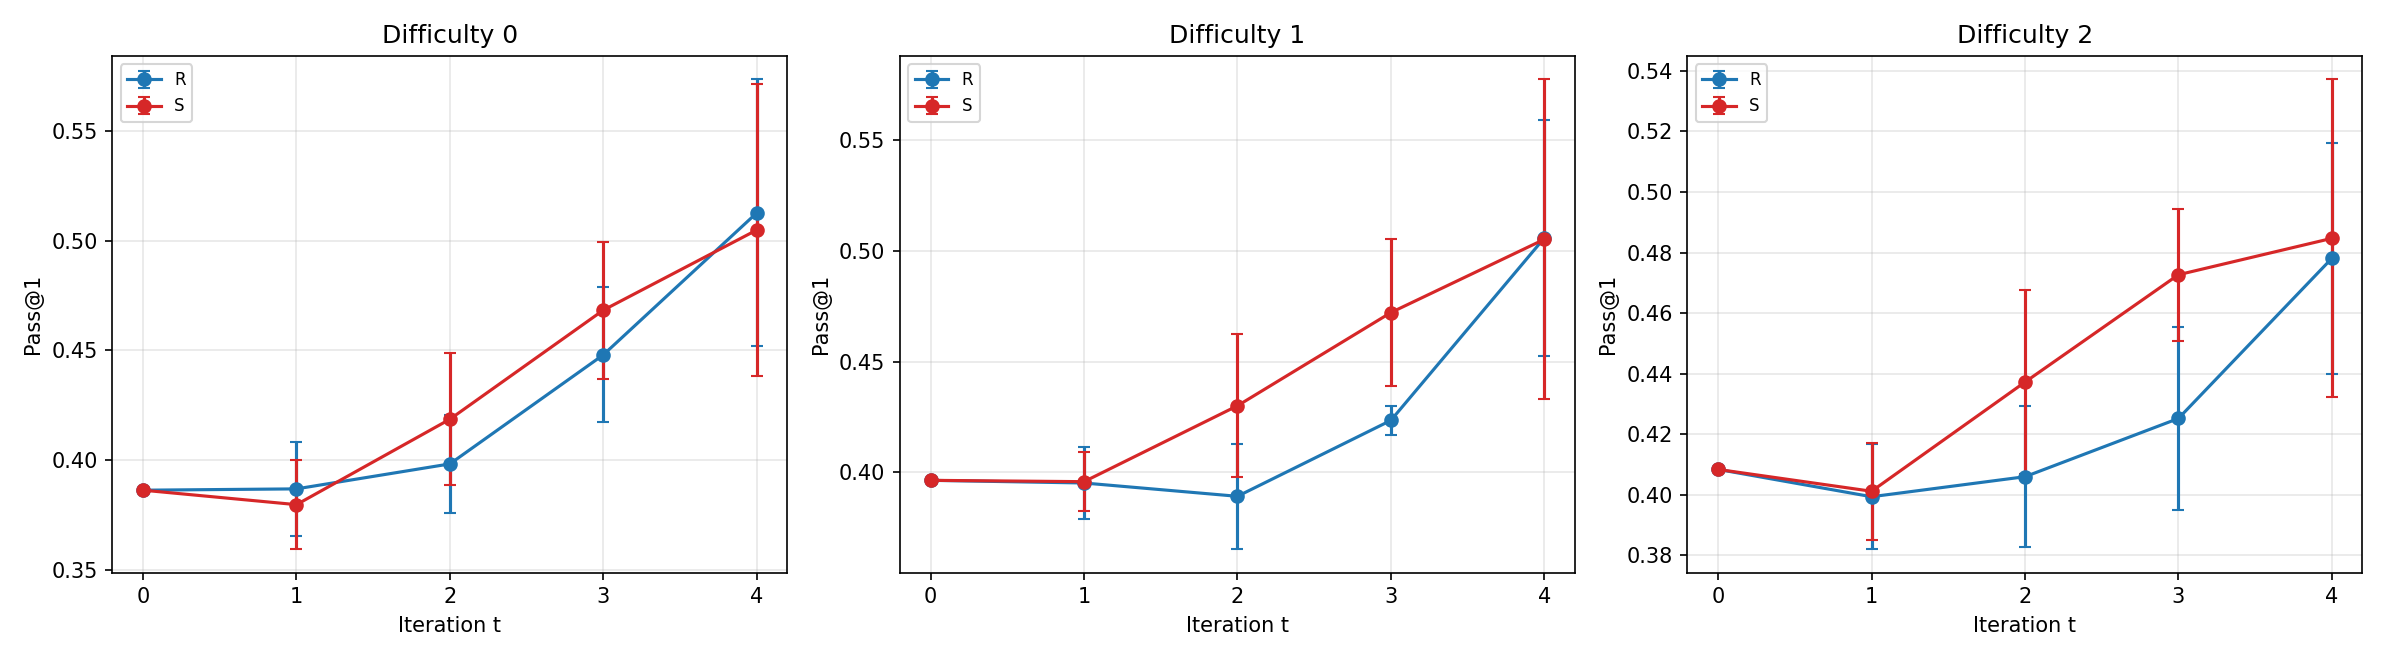
\includegraphics[width=0.90\linewidth]{figures/qwen4b_four_round_raw/unaudited_eval_ood_by_difficulty.png}
\caption{Original unaudited Qwen3-4B graph accuracy by generator
difficulty stratum, ID (top) and OOD (bottom), for rounds 0--4.
Strata 0--2 appear from left to right, containing $667/667/666$ ID
and $334/333/333$ OOD questions. Intervals use the same five blocks
as Figure~\ref{fig:qwen4b-raw-unaudited}.}
\label{fig:qwen4b-raw-unaudited-difficulty}
\end{figure}

The fixed generator strata do not establish a model-difficulty ordering.
Panel-specific vertical scales are retained, and these comparisons are
descriptive rather than multiplicity-adjusted. The breakdown provides
context for the aggregate trajectory without adding a stratum-level
accuracy claim.

\begin{figure}[H]
\centering
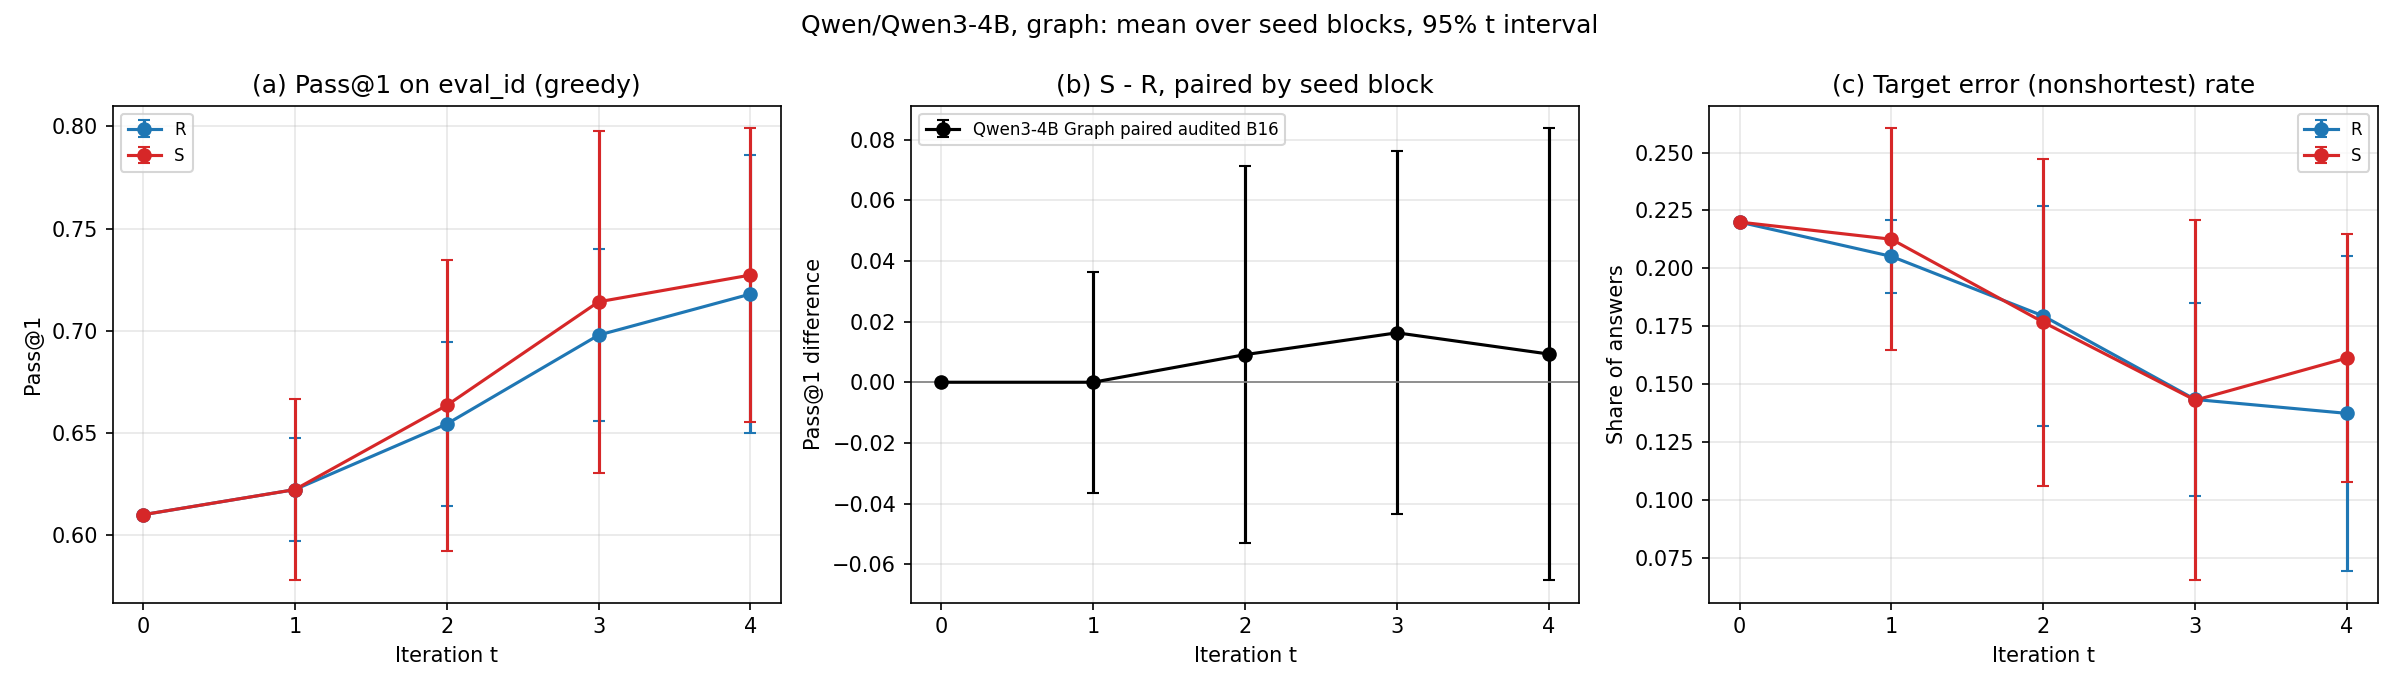
\includegraphics[width=0.90\linewidth]{figures/qwen4b_four_round_raw/audited_eval_id_pass1.png}
\par\smallskip
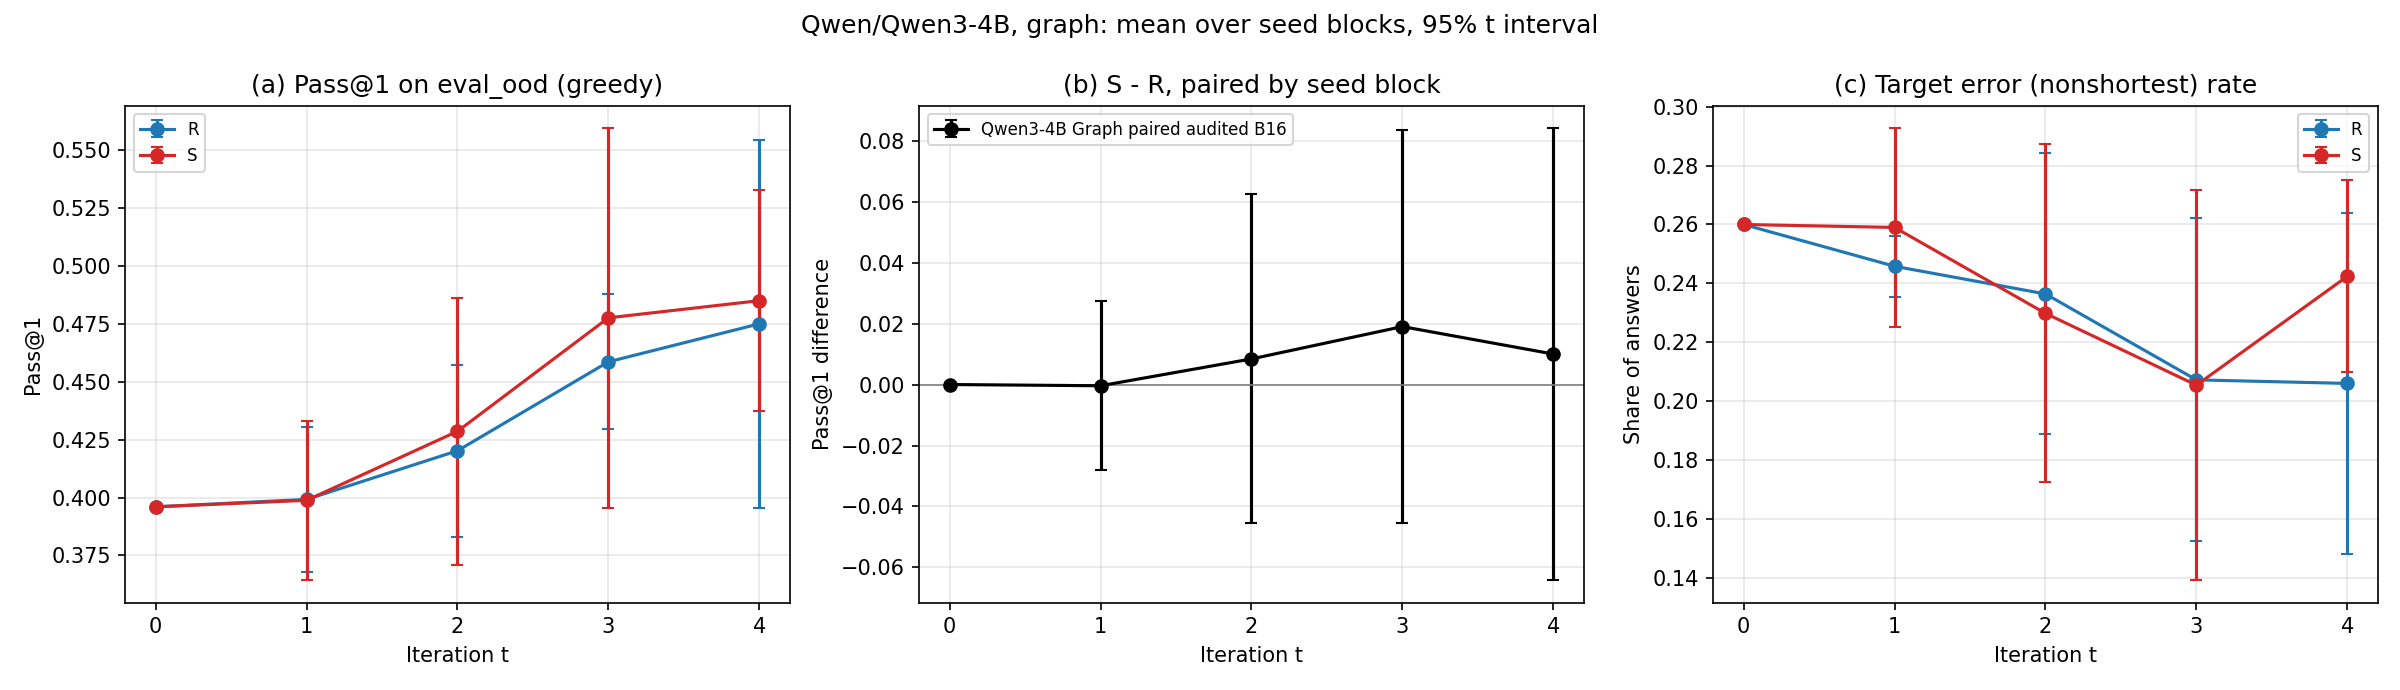
\includegraphics[width=0.90\linewidth]{figures/qwen4b_four_round_raw/audited_eval_ood_pass1.png}
\caption{Original adaptive-audit Qwen3-4B graph curves, ID (top)
and OOD (bottom), with 16 correctness queries per arm-round.
The panels show greedy Pass@1, paired $S-R$ accuracy, and
nonshortest-error incidence. Each audited arm spends 64 queries
over four rounds.}
\label{fig:qwen4b-raw-audited}
\end{figure}

Audited round-four $R/S$ accuracy is $0.7180/0.7273$ ID and
$0.4750/0.4850$ OOD, from audited-run bases $0.6100$ and $0.3960$.
The paired contrasts are $0.0093\pm0.0745$ and $0.0100\pm0.0741$.
They compare arms within the audited policy and
should not be interpreted as effects of auditing.

\begin{figure}[H]
\centering
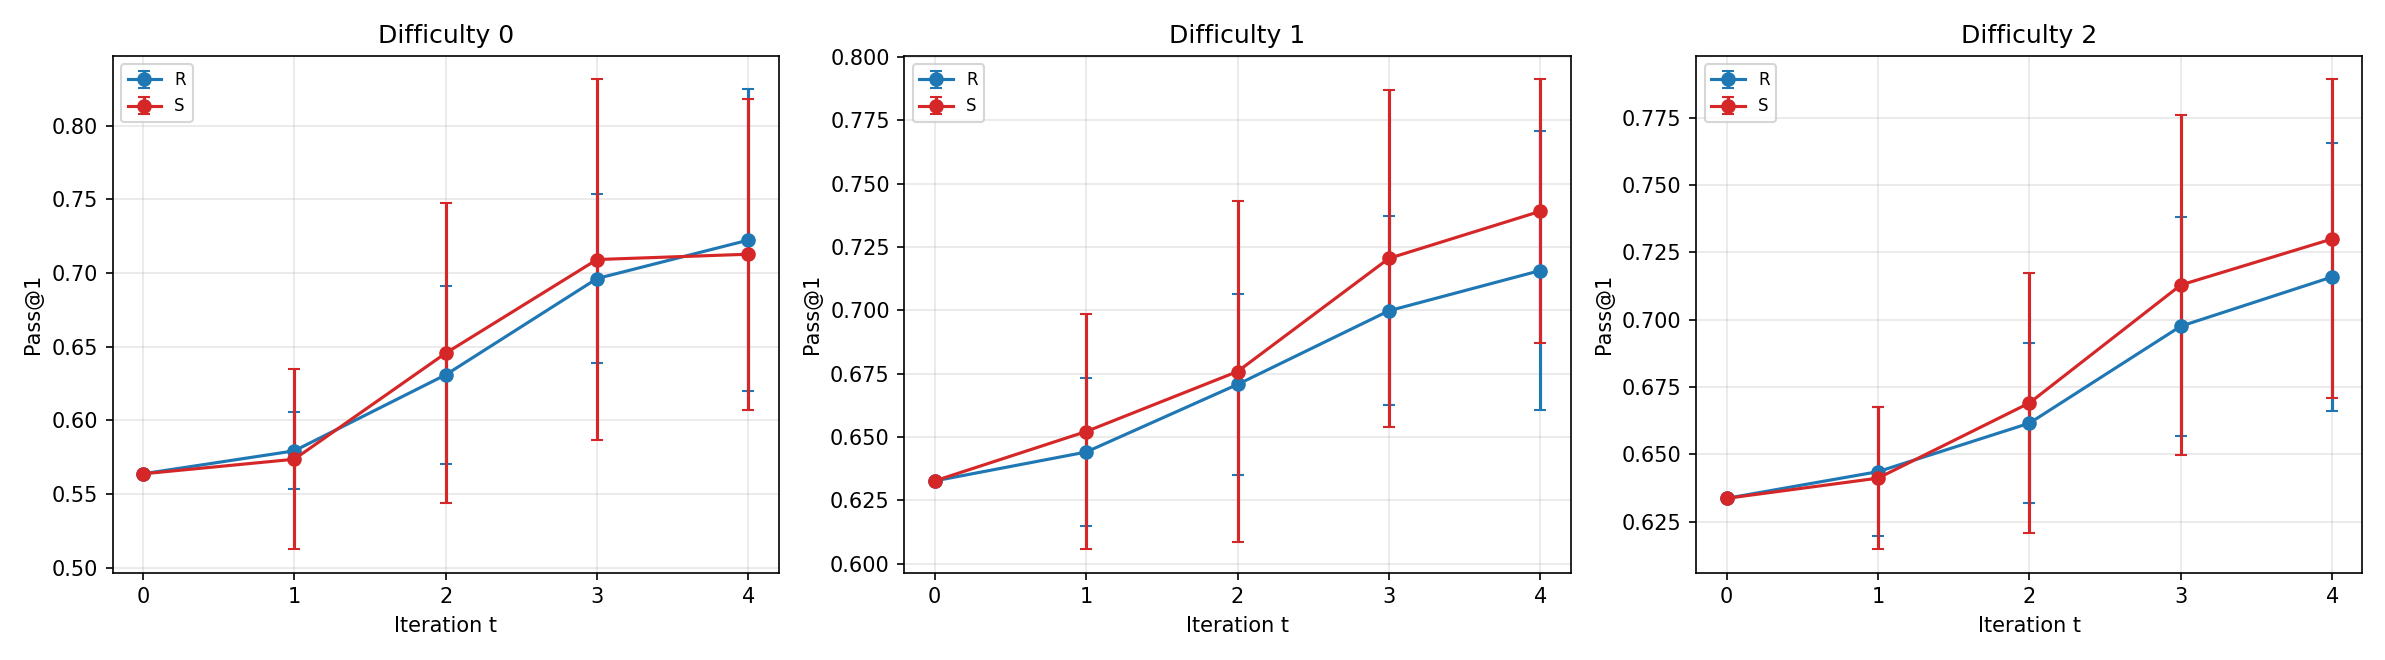
\includegraphics[width=0.90\linewidth]{figures/qwen4b_four_round_raw/audited_eval_id_by_difficulty.png}
\par\smallskip
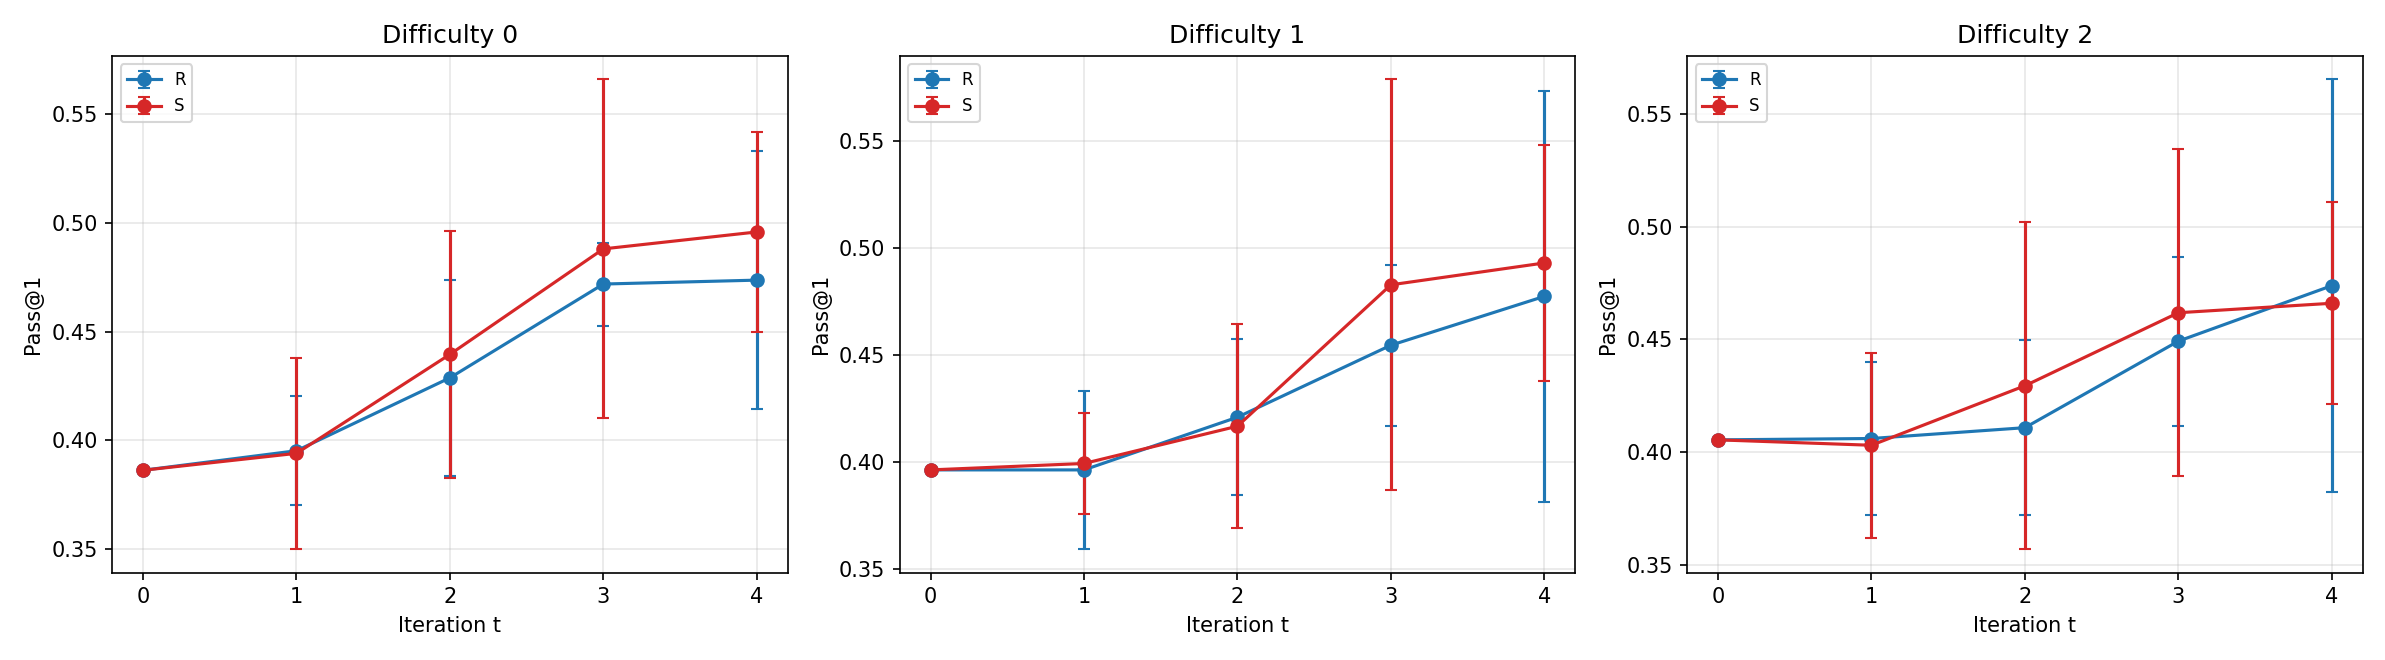
\includegraphics[width=0.90\linewidth]{figures/qwen4b_four_round_raw/audited_eval_ood_by_difficulty.png}
\caption{Original adaptive-audit Qwen3-4B graph accuracy by
generator stratum, ID (top) and OOD (bottom), for rounds 0--4.
Strata, fixed question sets, and interval conventions follow
Figure~\ref{fig:qwen4b-raw-unaudited-difficulty}.}
\label{fig:qwen4b-raw-audited-difficulty}
\end{figure}

The audited stratum curves use the same fixed questions and retain their
original panel-specific scales. They supplement the aggregate audited
results without establishing a stratum-specific audit benefit, which
would require a corresponding cross-policy comparison and treatment
of the multiple contrasts.

\begin{figure}[H]
\centering
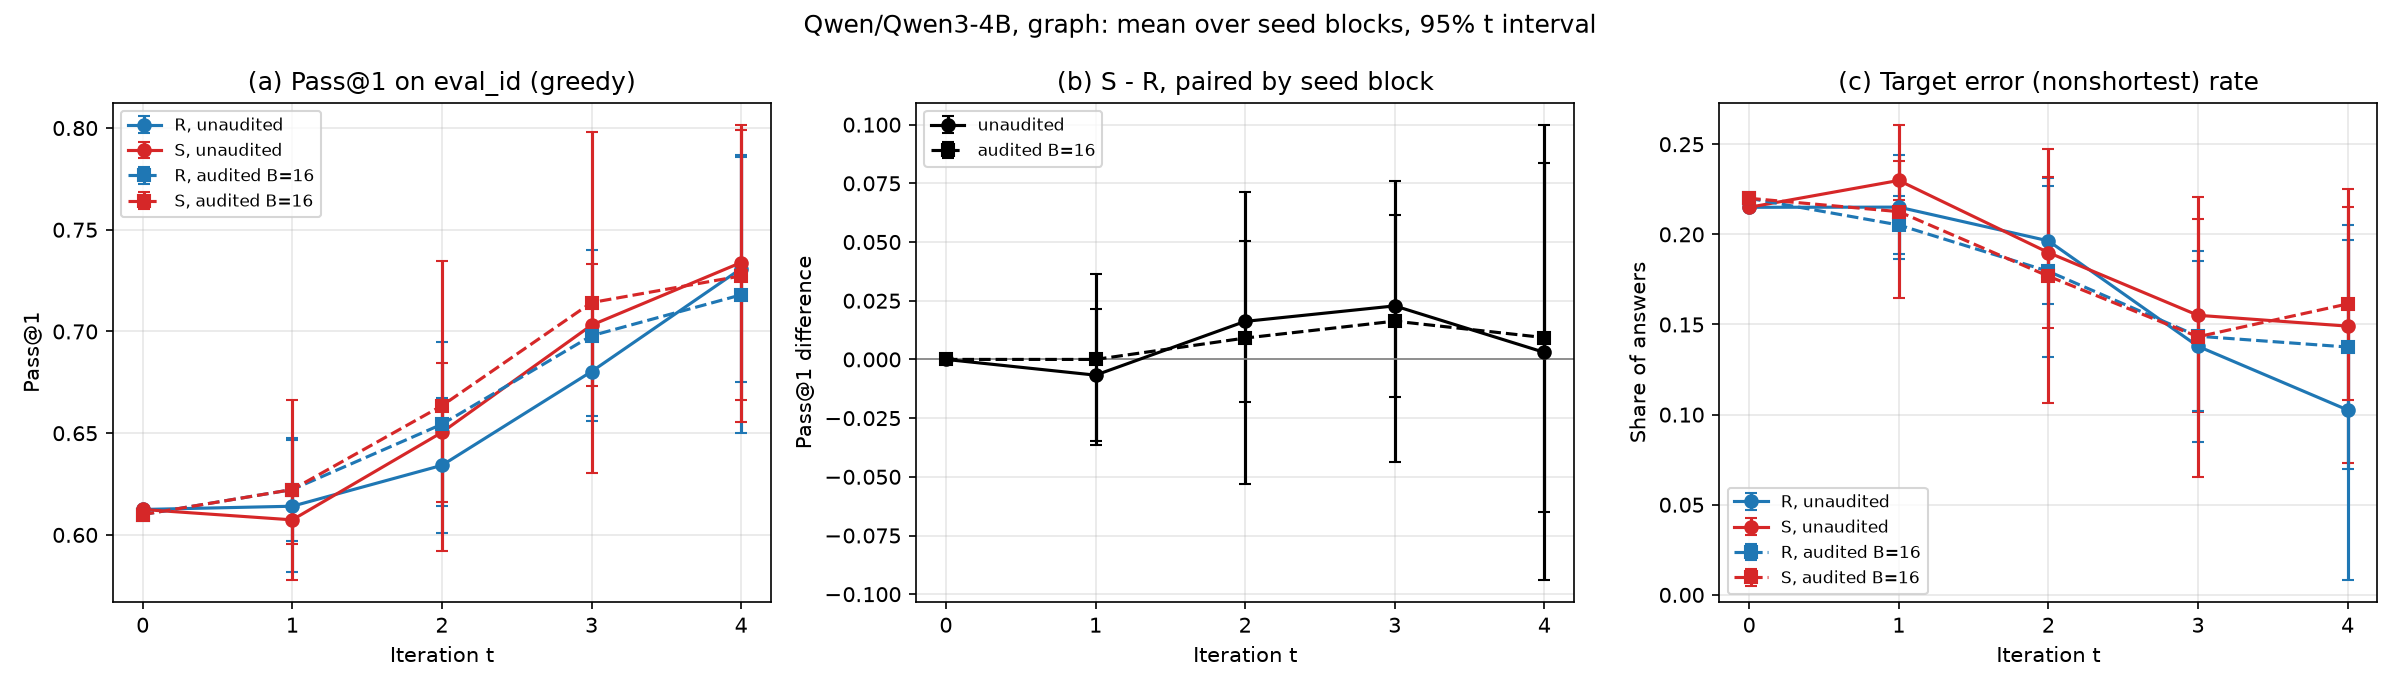
\includegraphics[width=0.90\linewidth]{figures/qwen4b_four_round_raw/comparison_eval_id_pass1.png}
\par\smallskip
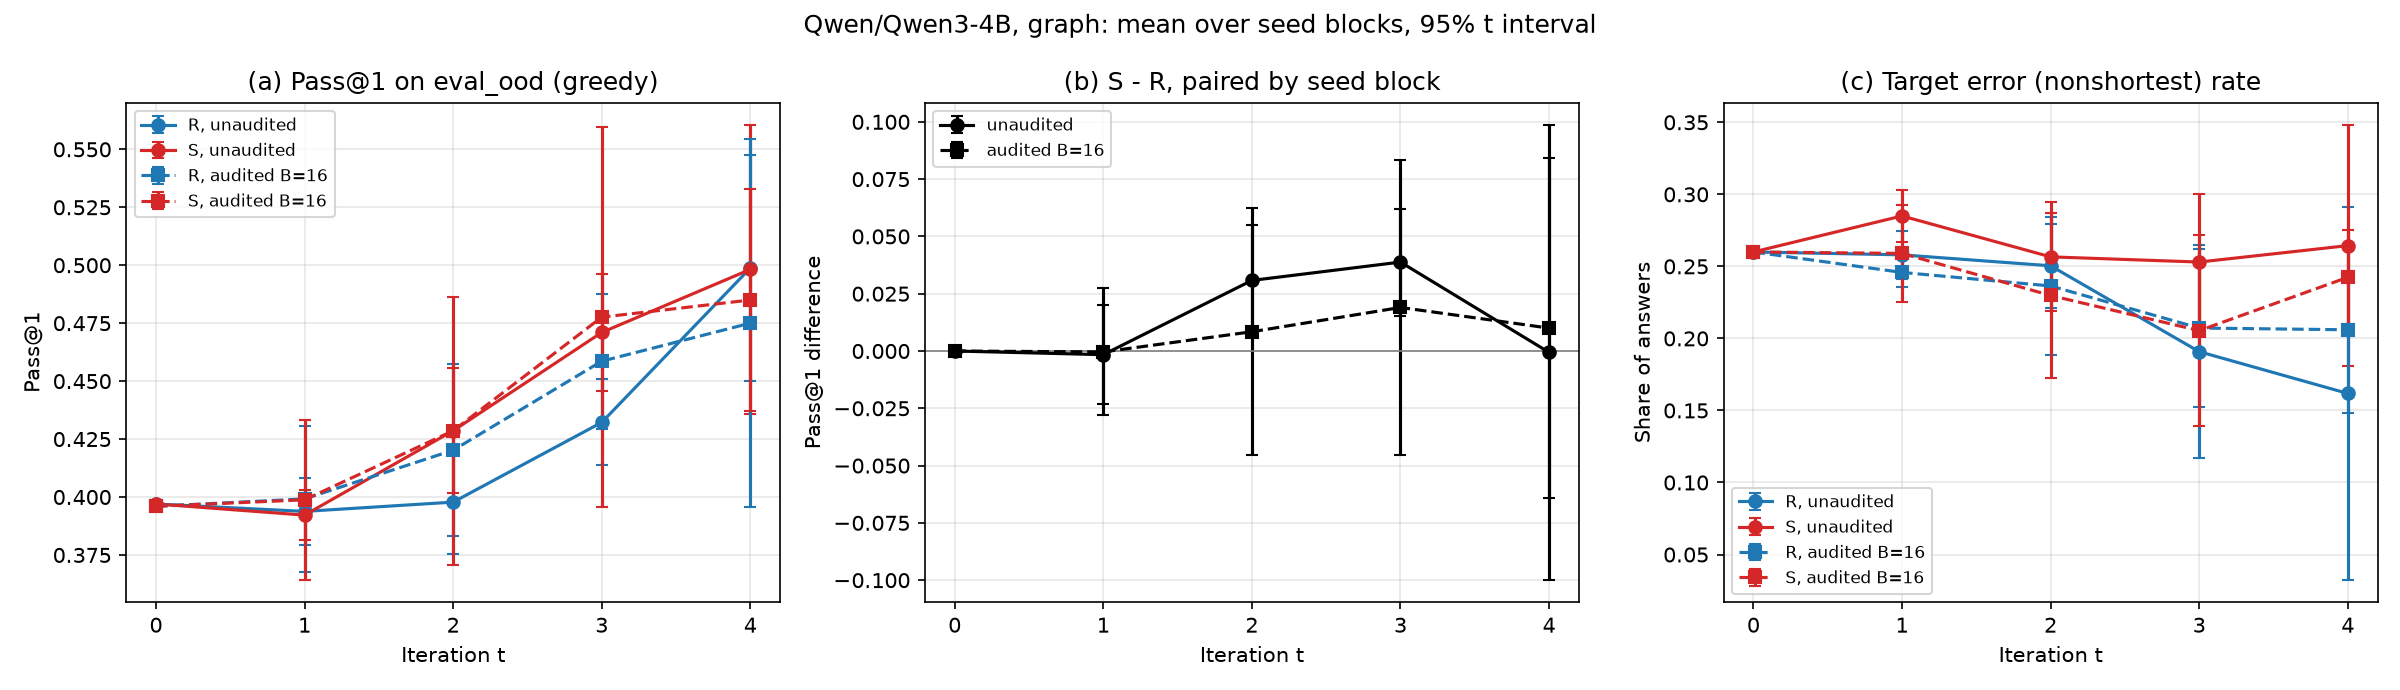
\includegraphics[width=0.90\linewidth]{figures/qwen4b_four_round_raw/comparison_eval_ood_pass1.png}
\caption{Joint Qwen3-4B graph trajectories, ID (top) and OOD
(bottom), generated with the original plotting method from the
same unaudited and audited checkpoints. The middle panels show
paired $S-R$ accuracy within each policy, not audited-minus-unaudited
effects.}
\label{fig:qwen4b-raw-comparison}
\end{figure}

Same-arm audit error changes are positive in mean
(Table~\ref{tab:audit-results}). Differences in optimizer effort
limit causal attribution: these results establish
neither an audit benefit nor a detrimental audit effect.

\begin{figure}[H]
\centering
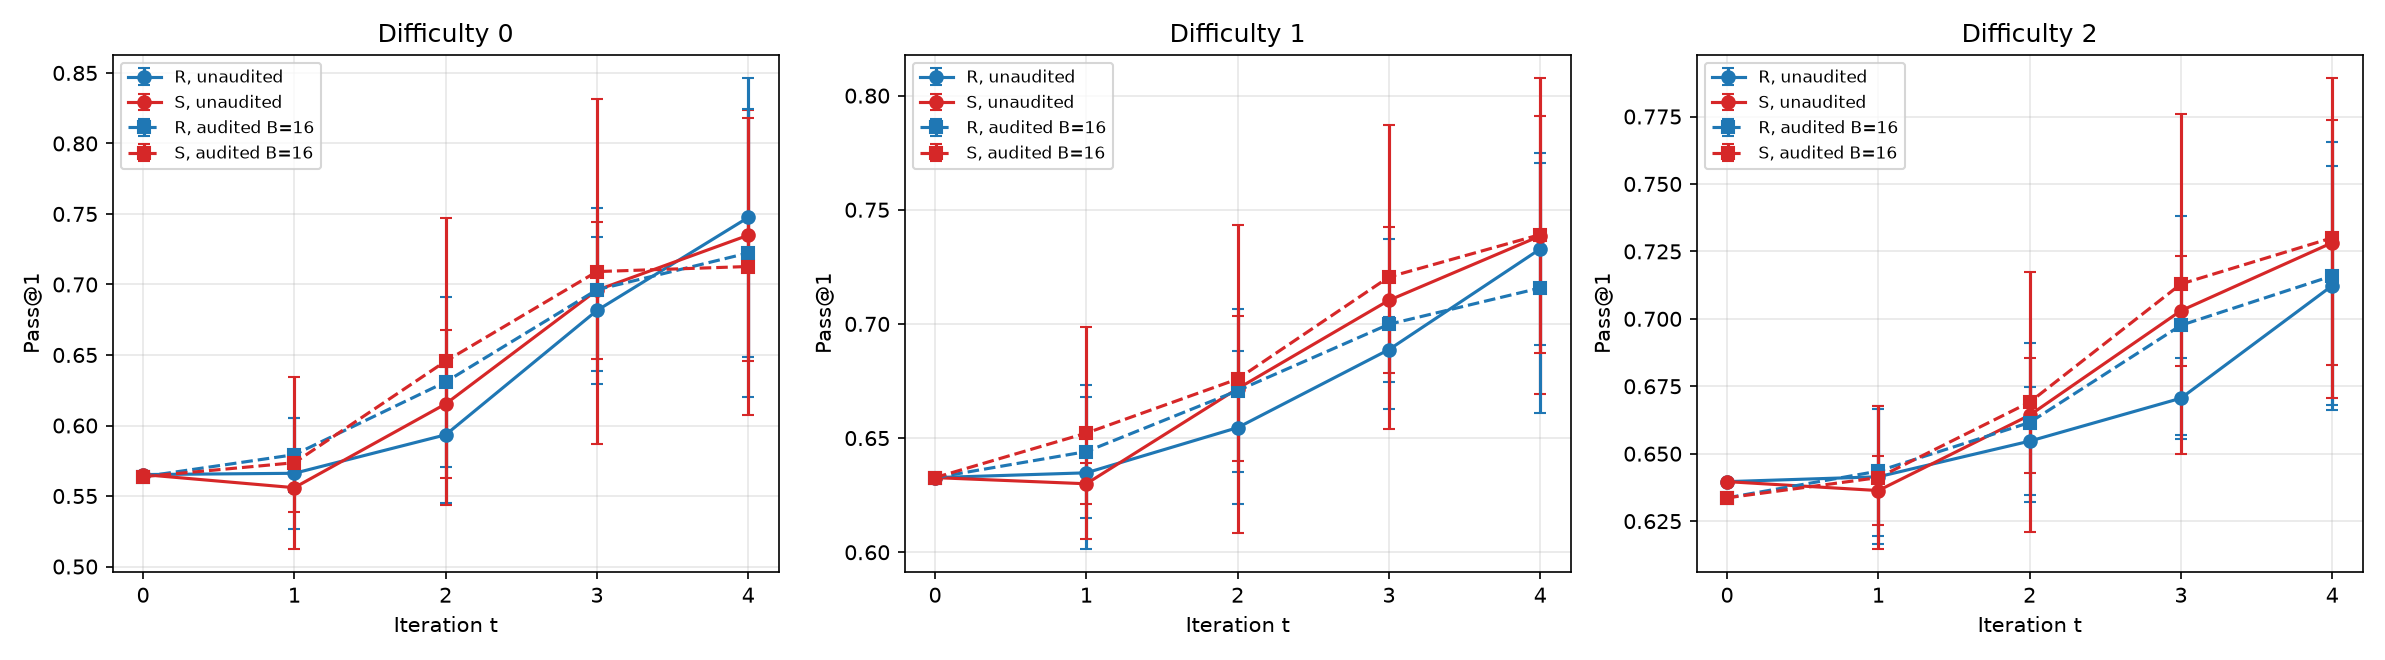
\includegraphics[width=0.90\linewidth]{figures/qwen4b_four_round_raw/comparison_eval_id_by_difficulty.png}
\par\smallskip
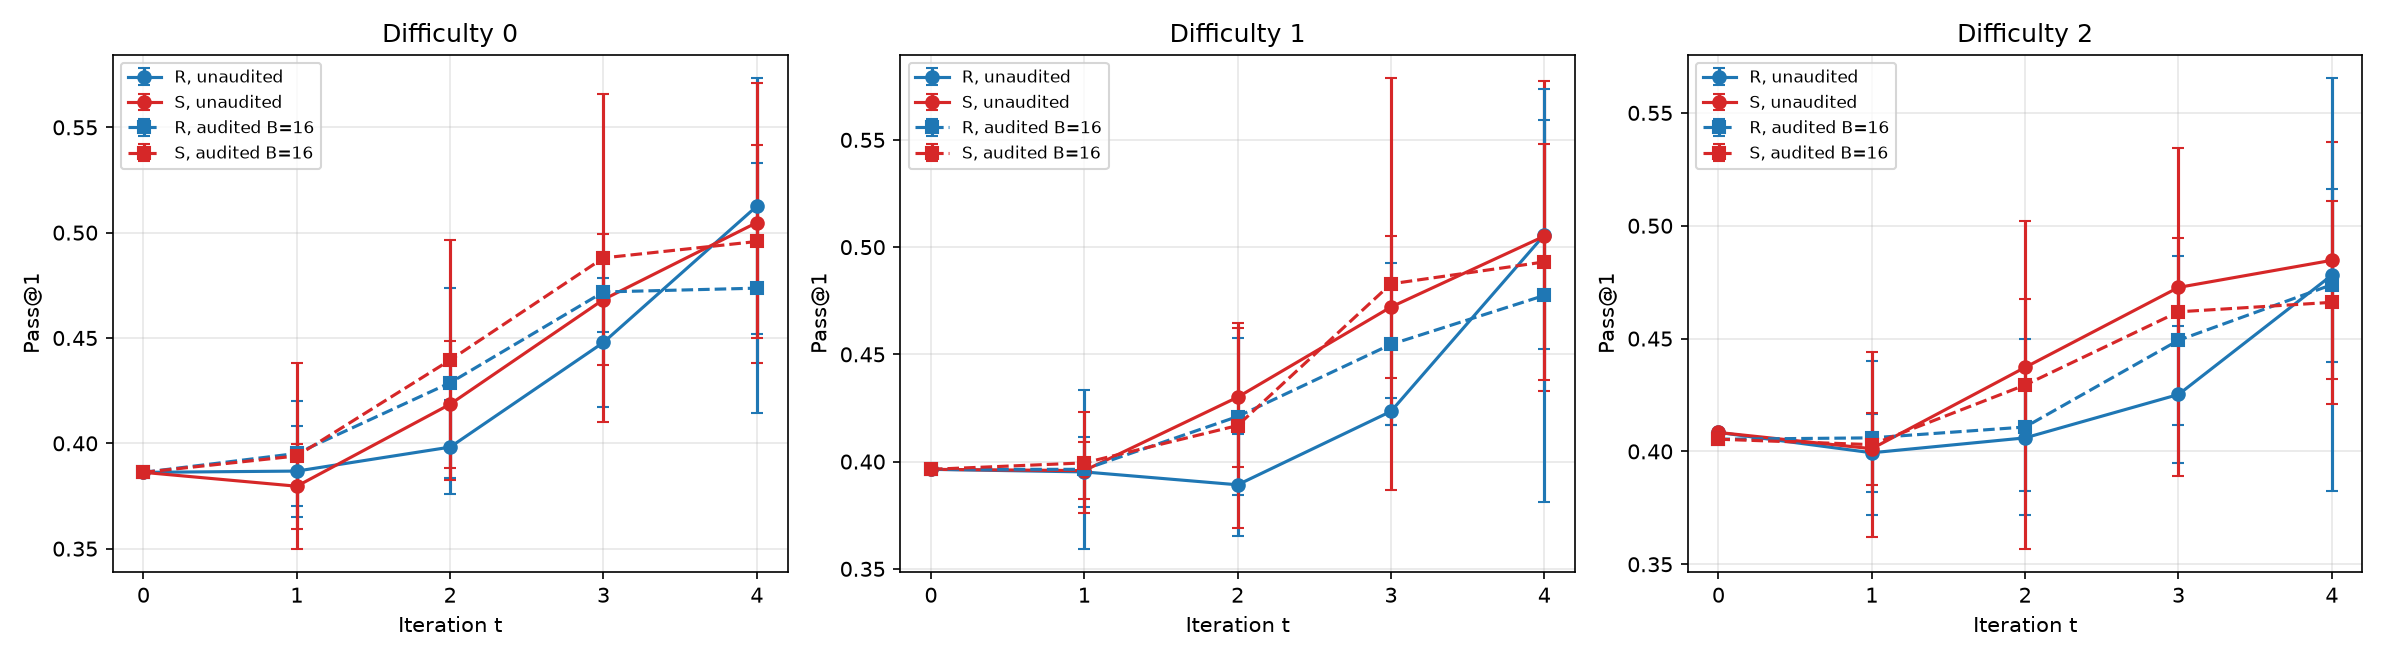
\includegraphics[width=0.90\linewidth]{figures/qwen4b_four_round_raw/comparison_eval_ood_by_difficulty.png}
\caption{Joint Qwen3-4B graph accuracy by generator stratum, ID
(top) and OOD (bottom), generated from the same checkpoint records
with the original plotting method. Both policies and arms use the
same question stratum at each checkpoint. Counts and interval
conventions follow Figure~\ref{fig:qwen4b-raw-unaudited-difficulty}.}
\label{fig:qwen4b-raw-comparison-difficulty}
\end{figure}

The two policies and arms share each question stratum. Panel-specific vertical scales are
unchanged, and the intervals are not adjusted across strata, rounds,
or policies. Consequently the joint breakdown remains descriptive,
consistent with the aggregate uncertainty rather than a separate
confirmatory analysis.
\endgroup



\subsection{Completed isolated one-step graph comparisons}
\label{app:one-step-results}

The isolated one-step graph studies are complete for Qwen3-1.7B,
Qwen3-4B, and Llama-3.2-3B-Instruct. Each uses five blocks, the original
matched round-one $K=64$ subsets, and one full-batch AdamW update per
$R/S$ arm at learning rate $5\times10^{-5}$, zero weight decay,
clipping threshold 1, and the same rank-8, $\alpha=16$, zero-dropout
\texttt{q\_proj}/\texttt{v\_proj} LoRA configuration. A dedicated
64-example reference gradient is bound to this configuration and initial
adapter; no multiround reference gradient is substituted. The null takes
zero updates and has exactly zero displacement and projection.
Table~\ref{tab:one-step-heldout} therefore reports measured one-step
outcomes, not first-round multistep results.

Table~\ref{tab:risk} brings together the one-step outcomes and update
diagnostics.
\begin{table}[H]
\caption{Unaudited one-step matrix. The three graph comparisons are complete: five paired blocks each, one AdamW update per $R/S$ arm, and an un-updated shared null. Separate rows identify the two arms. The primary paired contrast is $S-R$ in ID greedy Pass@1 (positive favors $S$), with a descriptive 95\% block-$t$ half-width, reported on the $S$ row. Multiround checkpoints are not substituted.}
\label{tab:risk}
\centering\small\setlength{\tabcolsep}{3pt}
\begin{tabular}{@{}lllcccccc@{}}
\toprule
Model & Task & Blocks & Arm & ID error & OOD error & \shortstack{ID Pass@1\\$S-R$} & $h^T\Delta\theta$ & $\|\Delta\theta\|_2$\\
\midrule
Qwen3-1.7B & Graph & 5 & $R$ & 0.4972 & 0.6470 & & $-0.00504$ & 0.0414\\
 & & & $S$ & 0.4970 & 0.6472 & $0.0002\pm0.0009$ & $-0.00540$ & 0.0414\\
\addlinespace
Qwen3-4B & Graph & 5 & $R$ & 0.3890 & 0.6040 & & $-0.00689$ & 0.0605\\
 & & & $S$ & 0.3896 & 0.6018 & $-0.0006\pm0.0036$ & $-0.00804$ & 0.0606\\
\addlinespace
Llama-3.2-3B & Graph & 5 & $R$ & 0.7502 & 0.7848 & & $-0.01850$ & 0.0478\\
 & & & $S$ & 0.7493 & 0.7838 & $0.0009\pm0.0028$ & $-0.01847$ & 0.0478\\
\addlinespace
Llama-3.2-3B & Arithmetic & 5 & --- & \TBD & \TBD & \TBD & \TBD & \TBD\\
Llama-3.2-1B & Arithmetic & 5 & --- & \TBD & \TBD & \TBD & \TBD & \TBD\\
\bottomrule
\end{tabular}
\end{table}


Protocol validation confirms complete evaluation of all eleven checkpoints
per split. Our analysis independently checks the available
training IDs, unit weights, 48/16 diagnostic label counts, matching
certificates, step counts, scalar diagnostic consistency, and held-out
count identities. It reproduces the supplied plot means, SDs and
paired intervals. Saved gradient-composition residuals are below the
recorded tolerance, but this scalar-record check does not reconstruct
the unavailable gradient or adapter tensors. Original execution checks
verified adapter identity; independent tensor-level verification requires
the unavailable adapters.

The Qwen3-1.7B comparison reuses its four-round study's initial inputs.
Qwen3-4B uses candidate pools generated without the repetition-stop rule;
matching and evaluation follow the specified one-step protocol. These
pools are not treated as newly sampled under a different stopping rule.
The one-step base accuracies are $0.4980/0.3530$ ID/OOD for Qwen3-1.7B,
$0.6145/0.3920$ for Qwen3-4B, and $0.2455/0.2070$ for Llama.
They differ slightly from the four-round baselines despite shared evaluation
question identities for the overlapping models. We use each run's own
null, not a baseline pooled across studies. Model-to-model differences
therefore do not constitute a controlled model-size comparison.

\begin{figure}[H]
\centering
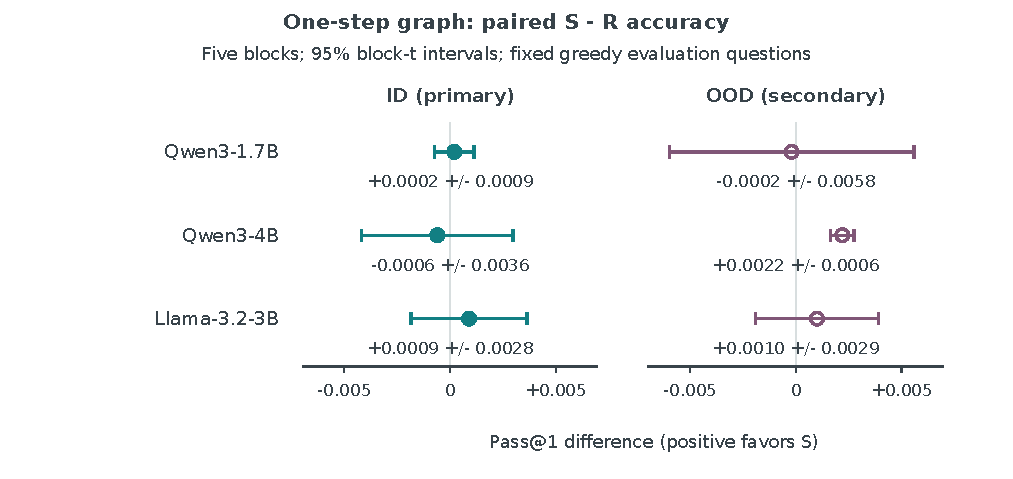
\includegraphics[width=0.85\linewidth]{figures/graph_extensions/one_step_contrasts.pdf}
\caption{Paired one-step graph accuracy contrasts $S-R$ in ID (primary)
and OOD (secondary), evaluated on each run's own fixed question sets.
Primary ID differences are $0.0002\pm0.0009$ for Qwen3-1.7B,
$-0.0006\pm0.0036$ for Qwen3-4B and $0.0009\pm0.0028$ for Llama.
Qwen3-4B's OOD difference is
$0.0022\pm0.0006$, with $S$ answering 2--3 more of the 1,000 OOD
questions correctly in every block. This secondary comparison is not
multiplicity-adjusted. Points and bars show means and descriptive 95\%
paired block-$t$ intervals over five blocks, not variation over model
initializations. Positive values favor $S$.}
\label{fig:one-step-contrasts}
\end{figure}

Relative to null, mean ID accuracy increases by
$0.0048/0.0050$ for Qwen3-1.7B $R/S$ and $0.0043/0.0052$ for Llama,
but decreases by $0.0035/0.0041$ for Qwen3-4B. Thus the common negative
mean reference projection is not a certificate of ID accuracy improvement.
For Qwen3-4B, the OOD advantage for $S$ is present in all five blocks;
the effect is small on the discrete question-count scale and remains a
secondary, unadjusted comparison.

Table~\ref{tab:one-step-diagnostics} decomposes the initial gradients
and reports actual displacement norms. Correct-gradient contributions
agree across arms, as expected from shared correct rows; the mean
error-gradient norm is larger in $S$ for all three models. This does not
alone determine an AdamW direction or prove that the targeted error
signature has higher reference-risk influence. Paired projection
contrasts are $-0.00035\pm0.00077$ (Qwen3-1.7B),
$-0.00115\pm0.00377$ (Qwen3-4B), and $0.00003\pm0.00063$ (Llama).
Both arms have negative projection in every
Qwen3-1.7B and Llama block; Qwen3-4B block \texttt{b00} has positive
projection in both arms. None of these pairs shows opposite projection
signs within a block.

Writing the LoRA correction as $(\alpha/r)BA$, the standard initialization
$B=0$ makes the initial gradient with respect to $A$ vanish.
For a fresh AdamW optimizer with zero weight
decay, bias correction gives the first update
$\Delta\theta=-\eta\,\widetilde g/(|\widetilde g|+\epsilon)$
coordinatewise, where $\widetilde g$ is the clipped gradient.
This is an ideal-arithmetic identity; it approximates a sign step only
when $|\widetilde g|\gg\epsilon$. Finite $\epsilon$ retains dependence
on gradient magnitude and clipping. The nearly equal $R/S$ displacement
norms therefore need not imply similar raw gradients.

\begin{table}[H]
\caption{One-step graph diagnostics at the shared initial adapter. $G_C$ and $G_E$ are correct/error contributions to the common full-batch gradient, not separately renormalized class means. Projections are surrogate first-order diagnostics, not certified reference-loss changes. Norms use measured AdamW displacements, not $-\eta G$. Clipping uses threshold 1.}
\label{tab:one-step-diagnostics}
\centering\small\setlength{\tabcolsep}{3pt}
\begin{tabular}{@{}llllllll@{}}
\toprule
Model & Arm & $h^T\Delta\theta$ & $\|\Delta\theta\|_2$ & $\|G_C\|_2$ & $\|G_E\|_2$ & $\|G\|_2$ & Clipped\\
\midrule
Qwen3-1.7B & R & $-0.00504\pm0.00217$ & 0.04139 & 0.8229 & 0.4366 & 0.9037 & 1/5\\
Qwen3-1.7B & S & $-0.00540\pm0.00230$ & 0.04139 & 0.8229 & 0.6204 & 0.9954 & 1/5\\
Qwen3-4B & R & $-0.00689\pm0.00969$ & 0.06054 & 0.4351 & 0.3051 & 0.5418 & 0/5\\
Qwen3-4B & S & $-0.00804\pm0.00722$ & 0.06055 & 0.4351 & 0.3186 & 0.5412 & 0/5\\
Llama-3.2-3B & R & $-0.01850\pm0.00244$ & 0.04782 & 0.5422 & 0.1847 & 0.6396 & 0/5\\
Llama-3.2-3B & S & $-0.01847\pm0.00261$ & 0.04782 & 0.5422 & 0.2030 & 0.6711 & 0/5\\
\bottomrule
\end{tabular}
\end{table}

\begin{table}[H]
\caption{Qwen3-1.7B one-step graph blocks. Each split uses the same fixed questions for its base/null and all ten trained checkpoints.}
\label{tab:one-step-blocks-graph_unaudited}
\centering\small\setlength{\tabcolsep}{3pt}
\begin{tabular}{@{}llllll@{}}
\toprule
Block & Arm & ID Pass@1 & OOD Pass@1 & $h^T\Delta\theta$ & $\|\Delta\theta\|_2$\\
\midrule
b00 & R & 0.5045 & 0.3530 & $-0.00589$ & 0.04138\\
b00 & S & 0.5040 & 0.3490 & $-0.00664$ & 0.04139\\
b01 & R & 0.5045 & 0.3560 & $-0.00515$ & 0.04139\\
b01 & S & 0.5045 & 0.3550 & $-0.00571$ & 0.04138\\
b02 & R & 0.5035 & 0.3520 & $-0.00467$ & 0.04140\\
b02 & S & 0.5030 & 0.3550 & $-0.00393$ & 0.04140\\
b03 & R & 0.5015 & 0.3550 & $-0.00712$ & 0.04138\\
b03 & S & 0.5025 & 0.3500 & $-0.00758$ & 0.04137\\
b04 & R & 0.5000 & 0.3490 & $-0.00238$ & 0.04138\\
b04 & S & 0.5010 & 0.3550 & $-0.00312$ & 0.04139\\
\bottomrule
\end{tabular}
\end{table}

\begin{table}[H]
\caption{Qwen3-4B one-step graph blocks. Each split uses the same fixed questions for its base/null and all ten trained checkpoints.}
\label{tab:one-step-blocks-graph_unaudited_qwen3-4b}
\centering\small\setlength{\tabcolsep}{3pt}
\begin{tabular}{@{}llllll@{}}
\toprule
Block & Arm & ID Pass@1 & OOD Pass@1 & $h^T\Delta\theta$ & $\|\Delta\theta\|_2$\\
\midrule
b00 & R & 0.6095 & 0.3950 & 0.00633 & 0.06046\\
b00 & S & 0.6115 & 0.3970 & 0.00054 & 0.06054\\
b01 & R & 0.6140 & 0.3970 & $-0.00944$ & 0.06050\\
b01 & S & 0.6090 & 0.3990 & $-0.00711$ & 0.06052\\
b02 & R & 0.6110 & 0.3970 & $-0.01158$ & 0.06060\\
b02 & S & 0.6120 & 0.3990 & $-0.01373$ & 0.06060\\
b03 & R & 0.6115 & 0.3980 & $-0.00653$ & 0.06055\\
b03 & S & 0.6095 & 0.4000 & $-0.00671$ & 0.06055\\
b04 & R & 0.6090 & 0.3930 & $-0.01323$ & 0.06058\\
b04 & S & 0.6100 & 0.3960 & $-0.01321$ & 0.06058\\
\bottomrule
\end{tabular}
\end{table}

\begin{table}[H]
\caption{Llama-3.2-3B one-step graph blocks. Each split uses the same fixed questions for its base/null and all ten trained checkpoints.}
\label{tab:one-step-blocks-graph_unaudited_llama3.2-3b}
\centering\small\setlength{\tabcolsep}{3pt}
\begin{tabular}{@{}llllll@{}}
\toprule
Block & Arm & ID Pass@1 & OOD Pass@1 & $h^T\Delta\theta$ & $\|\Delta\theta\|_2$\\
\midrule
b00 & R & 0.2490 & 0.2160 & $-0.01550$ & 0.04781\\
b00 & S & 0.2490 & 0.2150 & $-0.01526$ & 0.04781\\
b01 & R & 0.2510 & 0.2140 & $-0.01828$ & 0.04782\\
b01 & S & 0.2505 & 0.2170 & $-0.01892$ & 0.04782\\
b02 & R & 0.2505 & 0.2160 & $-0.01929$ & 0.04782\\
b02 & S & 0.2535 & 0.2160 & $-0.01952$ & 0.04781\\
b03 & R & 0.2475 & 0.2120 & $-0.01854$ & 0.04782\\
b03 & S & 0.2510 & 0.2160 & $-0.01782$ & 0.04782\\
b04 & R & 0.2510 & 0.2180 & $-0.02091$ & 0.04782\\
b04 & S & 0.2495 & 0.2170 & $-0.02085$ & 0.04782\\
\bottomrule
\end{tabular}
\end{table}


\begingroup
\let\figure\RSIappendixfigure
\let\endfigure\RSIendappendixfigure
\subsubsection{Block-level one-step errors and update projections}
\label{app:one-step-raw-figures}

Figures~\ref{fig:one-step-raw-qwen17}--\ref{fig:one-step-raw-llama}
show the original primary ID error-change and reference-projection plots
for the three completed one-step graph studies. These block-level views
complement the aggregate accuracy contrasts in
Figure~\ref{fig:one-step-contrasts} and Tables~\ref{tab:one-step-heldout}
and~\ref{tab:one-step-diagnostics}. Within each source plot, the left
panel connects $R/S$ observations from the same block; the right panel
shows the five paired $S-R$ differences and their mean with a descriptive
95\% block-$t$ interval. Null denotes the run's own unupdated adapter.
Error is $1-\mathrm{Pass@1}$, so its contrasts have the opposite sign
to accuracy contrasts. Projection is a first-order reference-loss
diagnostic, not a certified finite-step loss change or held-out task risk.
Original plots use separate vertical scales; no cross-model magnitude
comparison is inferred from their appearance.

\begin{figure}[H]
\centering
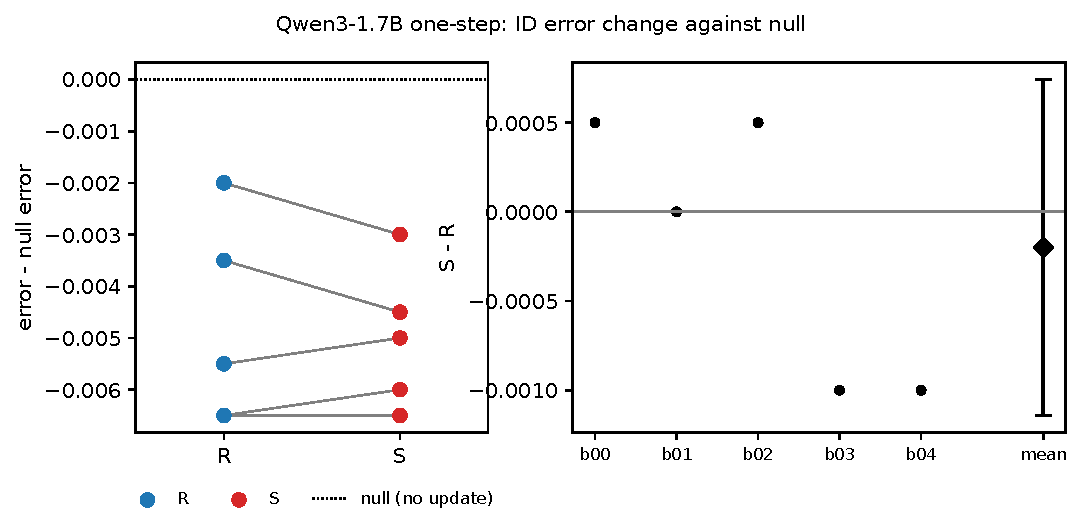
\includegraphics[width=0.82\linewidth]{figures/one_step_selected_raw/qwen3-1.7b_error_eval_id.pdf}
\par\smallskip
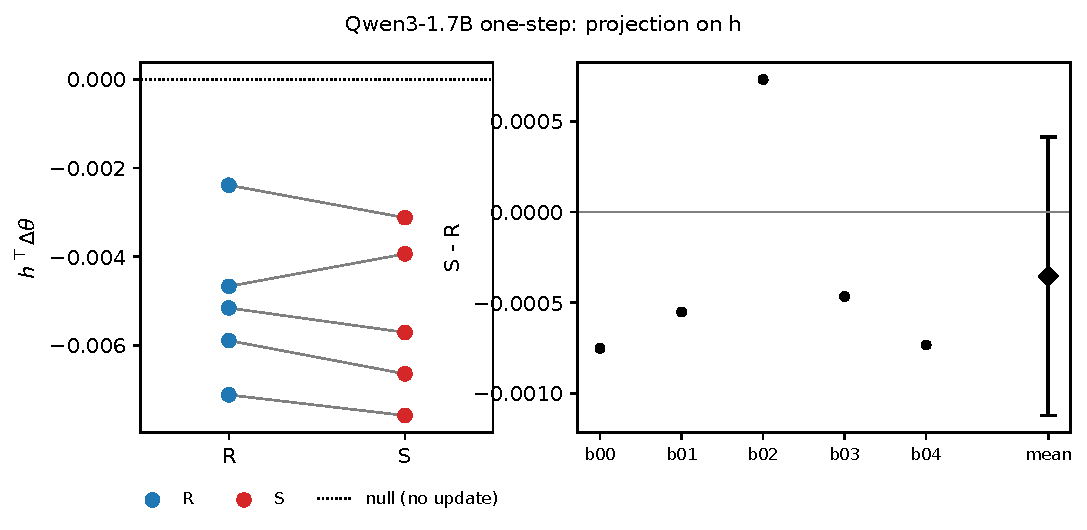
\includegraphics[width=0.82\linewidth]{figures/one_step_selected_raw/qwen3-1.7b_projection.pdf}
\caption{Original Qwen3-1.7B one-step ID error change against null
(top) and reference projection $h^T\Delta\theta$ (bottom), with five
paired blocks. The panels retain the run's own null as their reference.}
\label{fig:one-step-raw-qwen17}
\end{figure}

Both Qwen3-1.7B arms lower mean ID error relative to null, by
$0.0048/0.0050$ for $R/S$. The paired $S-R$ error contrast is
$-0.0002\pm0.0009$ and the projection contrast is
$-0.00035\pm0.00077$. Every block has
negative projection in both arms; none exhibits the theoretical
construction's opposite within-pair projection signs.

\begin{figure}[H]
\centering
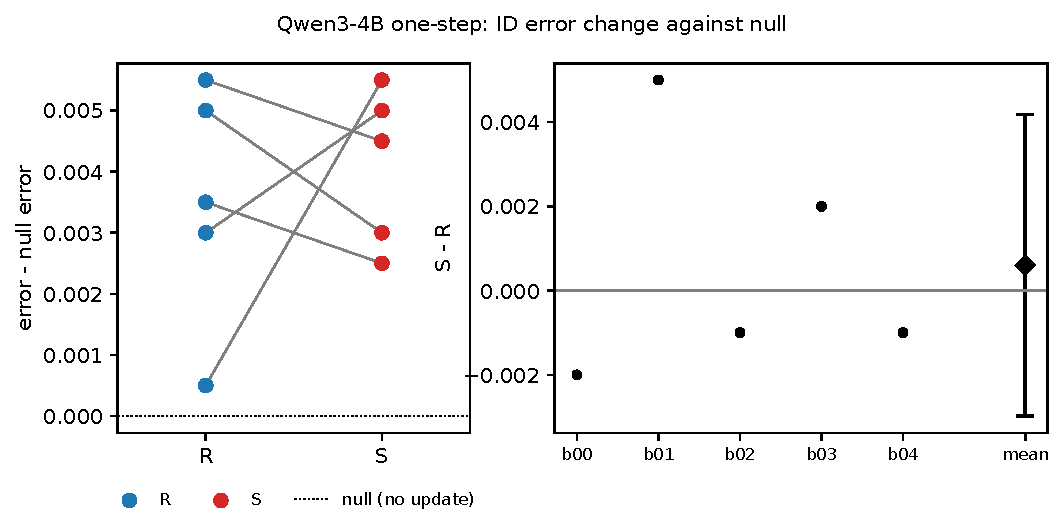
\includegraphics[width=0.82\linewidth]{figures/one_step_selected_raw/qwen3-4b_error_eval_id.pdf}
\par\smallskip
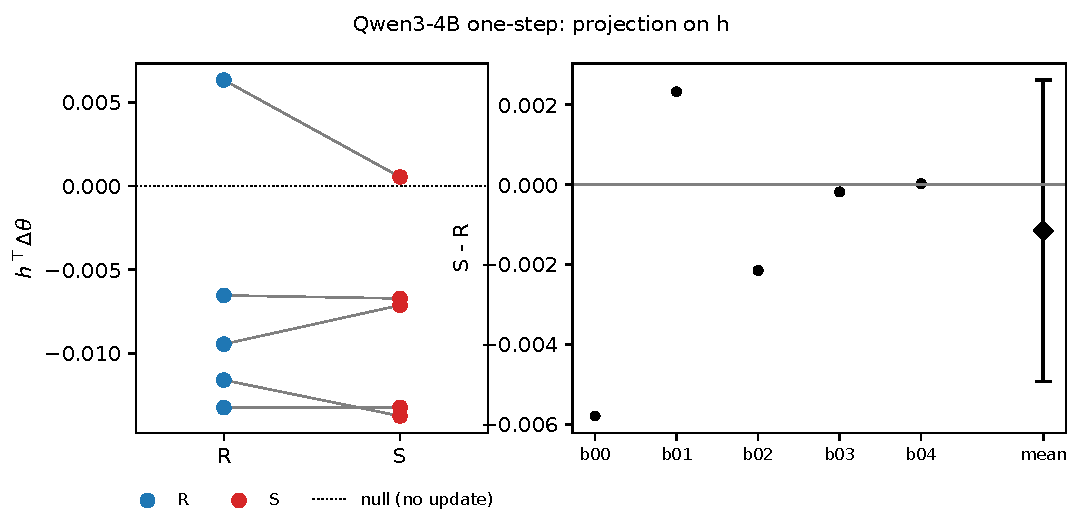
\includegraphics[width=0.82\linewidth]{figures/one_step_selected_raw/qwen3-4b_projection.pdf}
\caption{Original Qwen3-4B one-step ID error change against null
(top) and reference projection (bottom), with five paired blocks.
Error and projection are distinct outcomes and use separate scales.}
\label{fig:one-step-raw-qwen4}
\end{figure}

For Qwen3-4B, mean ID error increases by $0.0035/0.0041$ for $R/S$
despite negative mean projections. The paired contrasts are
$0.0006\pm0.0036$ for error and $-0.00115\pm0.00377$ for
projection. Block \texttt{b00} has positive
projection in both arms and the other four have negative projection
in both. A negative mean projection therefore does not certify
ID accuracy improvement.

\begin{figure}[H]
\centering
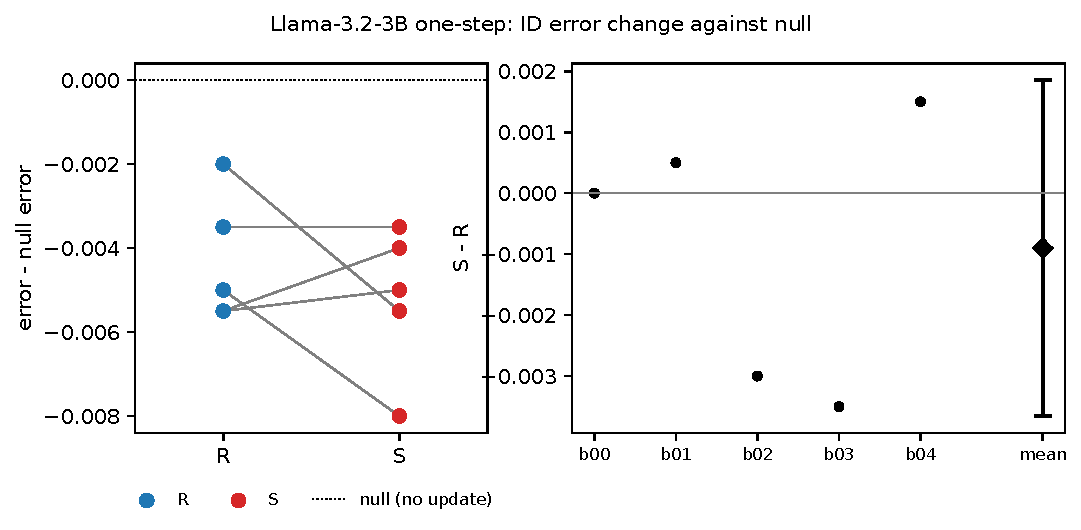
\includegraphics[width=0.82\linewidth]{figures/one_step_selected_raw/llama3.2-3b_error_eval_id.pdf}
\par\smallskip
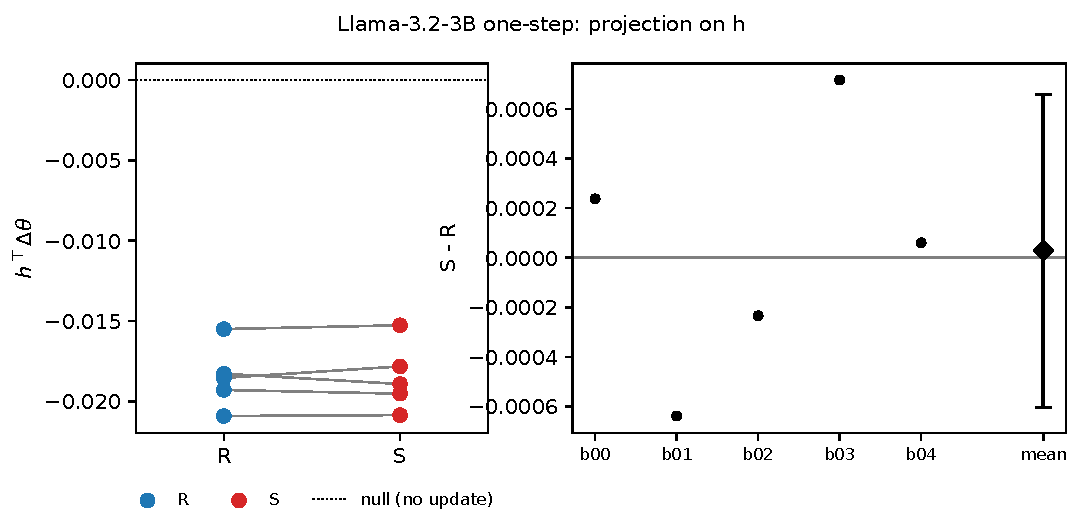
\includegraphics[width=0.82\linewidth]{figures/one_step_selected_raw/llama3.2-3b_projection.pdf}
\caption{Original Llama-3.2-3B-Instruct one-step ID error change
against null (top) and reference projection (bottom), with five
paired blocks.}
\label{fig:one-step-raw-llama}
\end{figure}

The Llama arms lower mean ID error by $0.0043/0.0052$ for $R/S$.
Paired contrasts are $-0.0009\pm0.0028$ for error and
$0.00003\pm0.00063$ for projection.
Every block has negative projection in both arms. These findings
do not establish equivalence of the arms or a within-pair directional
separation.
\endgroup


\paragraph{Validation and limits.}
Independent count-based checks reproduce the checkpoint metrics,
matching constraints, training and audit statistics, and paired contrasts
in the tables and figures. The figures preserve the underlying
observations and uncertainty. For these earlier exports, raw held-out answers,
adapter weights, and reference tensors are unavailable, so validation does
not include independent held-out rejudging, checkpoint reloading,
or tensor-level gradient recomputation. Qwen3-4B audited responses are
rejudged separately in Appendix~\ref{app:qwen4b-four-round}.
Run-specific baselines and reused
pools also prevent interpreting model-to-model differences as a controlled
model-size effect. Neither the finite-budget audit nor these one-step
diagnostics directly validate the population theorem's auditing policy.

